\PassOptionsToPackage{unicode=true}{hyperref} % options for packages loaded elsewhere
\PassOptionsToPackage{hyphens}{url}
\PassOptionsToPackage{dvipsnames,svgnames*,x11names*}{xcolor}
%
\documentclass[14pt,titlepage, oneside, openany, a4paper]{book}
\usepackage{lmodern}
\usepackage{setspace}
\setstretch{2}
\usepackage{amssymb,amsmath}
\usepackage{ifxetex,ifluatex}
\usepackage{fixltx2e} % provides \textsubscript
\ifnum 0\ifxetex 1\fi\ifluatex 1\fi=0 % if pdftex
  \usepackage[T1]{fontenc}
  \usepackage[utf8]{inputenc}
  \usepackage{textcomp} % provides euro and other symbols
\else % if luatex or xelatex
  \usepackage{unicode-math}
  \defaultfontfeatures{Ligatures=TeX,Scale=MatchLowercase}
\fi
% use upquote if available, for straight quotes in verbatim environments
\IfFileExists{upquote.sty}{\usepackage{upquote}}{}
% use microtype if available
\IfFileExists{microtype.sty}{%
\usepackage[]{microtype}
\UseMicrotypeSet[protrusion]{basicmath} % disable protrusion for tt fonts
}{}
\IfFileExists{parskip.sty}{%
\usepackage{parskip}
}{% else
\setlength{\parindent}{0pt}
\setlength{\parskip}{6pt plus 2pt minus 1pt}
}
\usepackage{xcolor}
\usepackage{hyperref}
\hypersetup{
            pdftitle={Introdução à análise de dados em R: Uma abordagem ambiental},
            pdfauthor={Wilson Souza \& Thiago Couto},
            colorlinks=true,
            linkcolor=blue,
            filecolor=Maroon,
            citecolor=Blue,
            urlcolor=blue,
            breaklinks=true}
\urlstyle{same}  % don't use monospace font for urls
\usepackage[left = 3cm, right = 2cm, top = 2.5cm, bottom = 3cm]{geometry}
\usepackage{color}
\usepackage{fancyvrb}
\newcommand{\VerbBar}{|}
\newcommand{\VERB}{\Verb[commandchars=\\\{\}]}
\DefineVerbatimEnvironment{Highlighting}{Verbatim}{commandchars=\\\{\}}
% Add ',fontsize=\small' for more characters per line
\usepackage{framed}
\definecolor{shadecolor}{RGB}{248,248,248}
\newenvironment{Shaded}{\begin{snugshade}}{\end{snugshade}}
\newcommand{\AlertTok}[1]{\textcolor[rgb]{0.94,0.16,0.16}{#1}}
\newcommand{\AnnotationTok}[1]{\textcolor[rgb]{0.56,0.35,0.01}{\textbf{\textit{#1}}}}
\newcommand{\AttributeTok}[1]{\textcolor[rgb]{0.77,0.63,0.00}{#1}}
\newcommand{\BaseNTok}[1]{\textcolor[rgb]{0.00,0.00,0.81}{#1}}
\newcommand{\BuiltInTok}[1]{#1}
\newcommand{\CharTok}[1]{\textcolor[rgb]{0.31,0.60,0.02}{#1}}
\newcommand{\CommentTok}[1]{\textcolor[rgb]{0.56,0.35,0.01}{\textit{#1}}}
\newcommand{\CommentVarTok}[1]{\textcolor[rgb]{0.56,0.35,0.01}{\textbf{\textit{#1}}}}
\newcommand{\ConstantTok}[1]{\textcolor[rgb]{0.00,0.00,0.00}{#1}}
\newcommand{\ControlFlowTok}[1]{\textcolor[rgb]{0.13,0.29,0.53}{\textbf{#1}}}
\newcommand{\DataTypeTok}[1]{\textcolor[rgb]{0.13,0.29,0.53}{#1}}
\newcommand{\DecValTok}[1]{\textcolor[rgb]{0.00,0.00,0.81}{#1}}
\newcommand{\DocumentationTok}[1]{\textcolor[rgb]{0.56,0.35,0.01}{\textbf{\textit{#1}}}}
\newcommand{\ErrorTok}[1]{\textcolor[rgb]{0.64,0.00,0.00}{\textbf{#1}}}
\newcommand{\ExtensionTok}[1]{#1}
\newcommand{\FloatTok}[1]{\textcolor[rgb]{0.00,0.00,0.81}{#1}}
\newcommand{\FunctionTok}[1]{\textcolor[rgb]{0.00,0.00,0.00}{#1}}
\newcommand{\ImportTok}[1]{#1}
\newcommand{\InformationTok}[1]{\textcolor[rgb]{0.56,0.35,0.01}{\textbf{\textit{#1}}}}
\newcommand{\KeywordTok}[1]{\textcolor[rgb]{0.13,0.29,0.53}{\textbf{#1}}}
\newcommand{\NormalTok}[1]{#1}
\newcommand{\OperatorTok}[1]{\textcolor[rgb]{0.81,0.36,0.00}{\textbf{#1}}}
\newcommand{\OtherTok}[1]{\textcolor[rgb]{0.56,0.35,0.01}{#1}}
\newcommand{\PreprocessorTok}[1]{\textcolor[rgb]{0.56,0.35,0.01}{\textit{#1}}}
\newcommand{\RegionMarkerTok}[1]{#1}
\newcommand{\SpecialCharTok}[1]{\textcolor[rgb]{0.00,0.00,0.00}{#1}}
\newcommand{\SpecialStringTok}[1]{\textcolor[rgb]{0.31,0.60,0.02}{#1}}
\newcommand{\StringTok}[1]{\textcolor[rgb]{0.31,0.60,0.02}{#1}}
\newcommand{\VariableTok}[1]{\textcolor[rgb]{0.00,0.00,0.00}{#1}}
\newcommand{\VerbatimStringTok}[1]{\textcolor[rgb]{0.31,0.60,0.02}{#1}}
\newcommand{\WarningTok}[1]{\textcolor[rgb]{0.56,0.35,0.01}{\textbf{\textit{#1}}}}
\usepackage{longtable,booktabs}
% Fix footnotes in tables (requires footnote package)
\IfFileExists{footnote.sty}{\usepackage{footnote}\makesavenoteenv{longtable}}{}
\usepackage{graphicx,grffile}
\makeatletter
\def\maxwidth{\ifdim\Gin@nat@width>\linewidth\linewidth\else\Gin@nat@width\fi}
\def\maxheight{\ifdim\Gin@nat@height>\textheight\textheight\else\Gin@nat@height\fi}
\makeatother
% Scale images if necessary, so that they will not overflow the page
% margins by default, and it is still possible to overwrite the defaults
% using explicit options in \includegraphics[width, height, ...]{}
\setkeys{Gin}{width=\maxwidth,height=\maxheight,keepaspectratio}
\setlength{\emergencystretch}{3em}  % prevent overfull lines
\providecommand{\tightlist}{%
  \setlength{\itemsep}{0pt}\setlength{\parskip}{0pt}}
\setcounter{secnumdepth}{5}
% Redefines (sub)paragraphs to behave more like sections
\ifx\paragraph\undefined\else
\let\oldparagraph\paragraph
\renewcommand{\paragraph}[1]{\oldparagraph{#1}\mbox{}}
\fi
\ifx\subparagraph\undefined\else
\let\oldsubparagraph\subparagraph
\renewcommand{\subparagraph}[1]{\oldsubparagraph{#1}\mbox{}}
\fi

% set default figure placement to htbp
\makeatletter
\def\fps@figure{htbp}
\makeatother

\usepackage{booktabs}
\usepackage{fullpage}
\usepackage{pdfpages}
\usepackage{amssymb}
\usepackage{graphicx}
\usepackage{geometry}
\usepackage[utf8]{inputenc}
\usepackage[portuguese]{babel}

%\lstset{
%  breaklines=true
%}
%\AtBeginDocument{\AtBeginShipoutNext{\AtBeginShipoutDiscard}}

\let\oldmaketitle\maketitle
\AtBeginDocument{\let\maketitle\relax}
\usepackage{booktabs}
\usepackage{longtable}
\usepackage{array}
\usepackage{multirow}
\usepackage{wrapfig}
\usepackage{float}
\usepackage{colortbl}
\usepackage{pdflscape}
\usepackage{tabu}
\usepackage{threeparttable}
\usepackage{threeparttablex}
\usepackage[normalem]{ulem}
\usepackage{makecell}
\usepackage{xcolor}
\usepackage[]{natbib}
\bibliographystyle{apalike}

\title{Introdução à análise de dados em R: Uma abordagem ambiental}
\author{Wilson Souza \& Thiago Couto}
\date{}

\begin{document}
\maketitle

%\cleardoublepage\newpage\thispagestyle{empty}\null
%\cleardoublepage\newpage\thispagestyle{empty}\null
%\cleardoublepage\newpage\thispagestyle{empty}
%\cleardoublepage\newpage\thispagestyle{empty}\null
%\cleardoublepage\newpage\thispagestyle{empty}\null
%\thispagestyle{empty}

\begin{figure}
  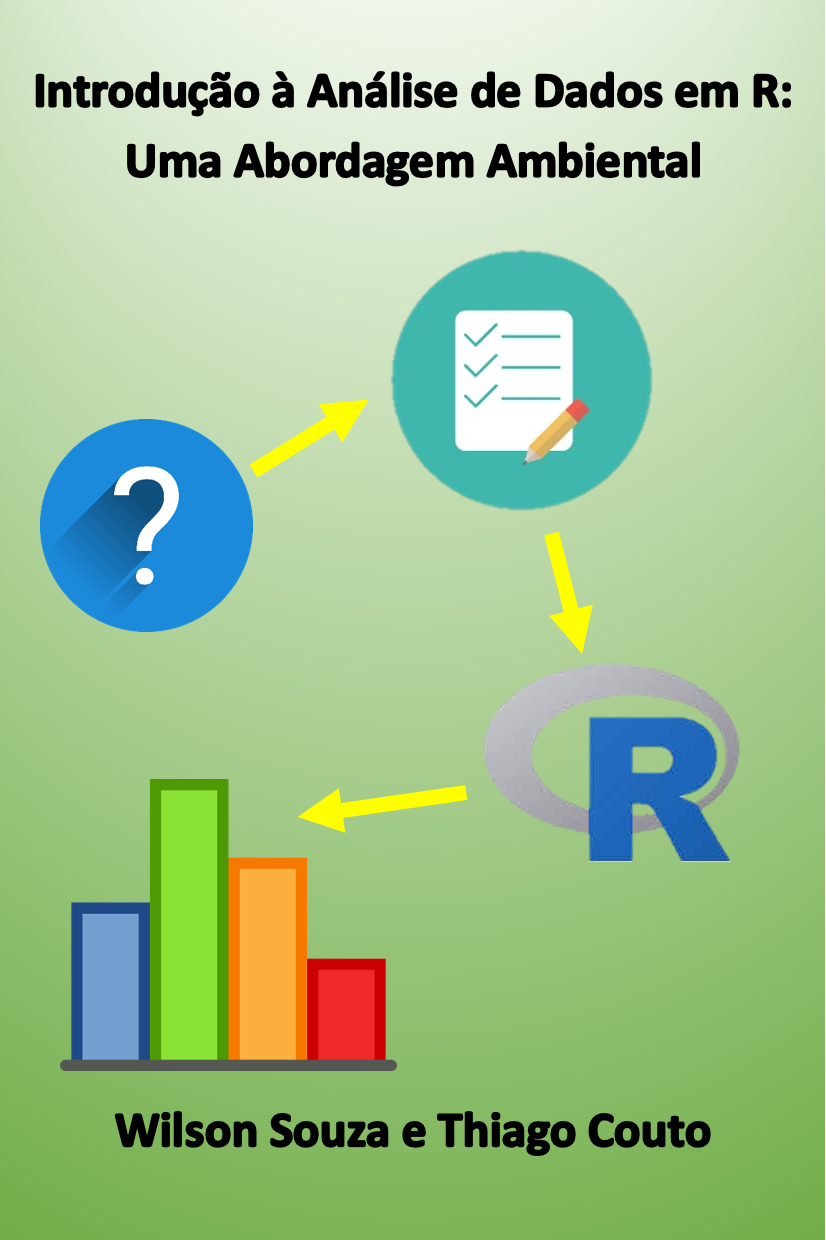
\includepdf[scale = 1.1]{cover.pdf}
\end{figure}

\let\maketitle\oldmaketitle
\maketitle

\renewcommand*\contentsname{Índice}
{
\hypersetup{linkcolor=}
\setcounter{tocdepth}{1}
\tableofcontents
}
\listoftables
\listoffigures
\hypertarget{prefuxe1cio}{%
\chapter*{Prefácio}\label{prefuxe1cio}}
\addcontentsline{toc}{chapter}{Prefácio}

\hypertarget{estrutura-do-livro}{%
\section*{Estrutura do livro}\label{estrutura-do-livro}}
\addcontentsline{toc}{section}{Estrutura do livro}

Este livro é composto de 4 capítulos, com diversos exemplos e todos com exercícios. O capítulo 1 traz uma breve explicação sobre a linguagem R, as vantagens do uso de sua interface gráfica RStudio, assim como do uso dessa ferramenta para análise de dados. Iremos, ainda neste capítulo, explorar as principais guias do RStudio, como elas estão organizadas e quais as suas principais funcionalidades. O capítulo 2 vem demonstrar como se dá o processo de importação de um conjunto de dados para o RStudio por diferentes meios (linhas de comando e interface gráfica), Fazer a verificação e ajuste dos dados, sumarizar os dados estatisticamente tanto por suas métricas quanto por gráficos, usando os pacotes básicos do R. O capítulo 3 traz a análise do qui-quadrado, tanto para ajuste das frequências quanto para o teste de independência e é apresentado brevemente a construção de suas hipóteses nulas e em detalhes o seu resultado. O capítulo 4 traz a análise do teste-t para uma amostra, duas amostras e pareado os quais, também, tem suas hipóteses apresentadas e detalhamento de seus resultados e a análise de seus pressupostos. Ao fim do livro é disponibilizado um apêndice com a resposta para os exercícios.

Alumas marcações são feitas no livro para melhor apresentação, tais como: Nomes de funções estão em azul; Nomes dos pacotes estão em marrom; Observações estão em vermelho; Objetos estão em negrito; Argumentos estão entre aspas; Operadores matemáticos estão em negrito e entre aspas; Nomes em inglês estão em itálico; Classes dos objetos estão em itálico\footnote{pois são nomes em inglês e não iremos detalha-las só reforça-las quando fatores};

\hypertarget{agradecimentos}{%
\section*{Agradecimentos}\label{agradecimentos}}
\addcontentsline{toc}{section}{Agradecimentos}

Em primeiro lugar só podemos agradecer a nossa família, pois são quem estão ao nosso lado a todo instante nos dando suporte. Em segundo lugar gostaríamos de agradecer a todos os professores pois foram eles que nos deram a base necessária para que esse livro viesse a existir. Em terceiro lugar gostaríamos de agradecer ao Rodrigo Luiz Lisboa Leitão por seus valiosos comentários e revisão dos capítulos 1 e 2. Por último e não menos importante gostaríamos de agradecer a vocês que estão utilizando o conhecimento presente aqui, porque é para vocês que este livro foi construído.

\hypertarget{sobre-os-autores}{%
\chapter*{Sobre os autores}\label{sobre-os-autores}}
\addcontentsline{toc}{chapter}{Sobre os autores}

\textbf{Wilson Souza}

Possui graduação em Licenciatura Plena em Ciências Biológicas pela Universidade Federal do Rio de Janeiro (UFRJ) com dupla diplomação com a Universidade de Coimbra (UC) - Portugal, Bacharelado em Biologia Marinha pela Universidade Federal do Rio de Janeiro (UFRJ) e Mestrado em Oceanografia Biológica pela Universidade Federal do Rio Grande (FURG). Desde 2012 trabalha em projetos de monitoramento de populações de camarões com foco em aspectos ecológicos e pesqueiros e em projetos de ecologia do benthos marinho. Aprendeu a linguagem R durante o mestrado e desde então tem se dedicado a ampliar seus conhecimentos em análise de dados voltado para monitoramento ambiental e aspectos ecológicos do benthos marinho.

\textbf{Thiago Couto}

Possui graduação em Ciências Biológicas pela Universidade Santa Úrsula, Mestrado em Ecologia pela Universidade de Coimbra -- Portugal, Doutorado em Biociências com especialização em Ecologia Marinha também pela Universidade de Coimbra -- Portugal e Pós-Doutorado em Oceanografia Biológica pela Universidade Federal do Rio de Janeiro. Em sua vida acadêmica já trabalhou com avaliação da qualidade ambiental usando organismos bentônicos, sequestro de carbono em vegetação de marisma, monitoramento ambiental, entre outras coisas. Nos últimos anos têm se dedicado ao monitoramento ambiental de costões rochosos e análise de risco de espécies invasoras.

\hypertarget{r}{%
\chapter{R}\label{r}}

\hypertarget{o-que-uxe9}{%
\section{O que é?}\label{o-que-uxe9}}

É uma linguagem de programação derivada da linguagem S (1976) e desenvolvida na Bell Laboratories (Atualmente Lucen Technologies) pelo estatístico John McKinley Chambers e colaboradores a qual no início da década de 90 foi implementada pelos estatísticos Ross Ihaka e Robert Gentleman e liberada oficialmente como linguagem R em 1995, sendo a primeira versão estável liberada em 2000 e tem sido constantemente atualizada. Atualmente tem se tornado a principal ferramenta para análise de dados, tanto em meio acadêmico quanto empresarial, principalmente devido ao seu caráter \emph{open-source} (código aberto).

Para maiores informações acesse o site do projeto R em: \url{https://www.r-project.org/about.html}.

\hypertarget{porque-usar-o-r-para-anuxe1lise-de-dados}{%
\section{Porque usar o R para análise de dados?}\label{porque-usar-o-r-para-anuxe1lise-de-dados}}

A estatística é uma ferramenta essencial para entendermos melhor os ecossistemas que estudamos. Com ela podemos compreender melhor os dados que coletamos, sejam dados biológicos ou ambientais tanto no âmbito de organismos microscópicos como macroscópicos.

Existe uma grande variedade de programas estatísticos que podem satisfazer nossas necessidades de análise dos nossos dados (Statistica, SPSS, past, Primer-E etc). Então, porque devemos usar o programa R?

Primeiramente, o R é gratuito, enquanto a maioria dos outros programas disponíveis no mercado não são baratos podendo a chegar a valores próximo de \$6000,00 doláres a assinatura por ano, como no caso do programa SPSS. Em segundo lugar, no R é possível fazer todas as análises que os outros programas fazem, portanto, não é necessário ter mais de um programa para se realizar diversas análises.

Vocês podem estar se perguntando se terão que aprender programação para trabalhar com R. A resposta é sim e não. As análises feitas no R são realizadas através de linhas de comando como em uma linguagem de programação, porém modificada, de mais fácil compreensão e intuítiva. Todavia, nosso objetivo com esta obra é facilitar o seu aprendizado desta linguagem para o universo da análise de dados, por meio de questões e exemplos pertinentes a área ambiental. Por outro lado, é preciso saber como o R se estrutura e funciona, pois um pequeno erro na escrita pode fazer com que a análise não funcione adequadamente. Mas não se preocupe iremos tentar facilitar para você.

Portanto, neste livro mostraremos desde como se importar uma tabela até fazer algumas análises estatísticas e gráficos que são vastamente utilizados na área ambiental.

\hypertarget{o-rstudio}{%
\section{O RStudio}\label{o-rstudio}}

O RStudio foi construído especificamente para a linguagem R e é um ambiente de desenvolvimento integrado (no inglês IDE) (Figura \ref{fig:RStudio}). Ele fornece uma interface gráfica (visa facilitar ao usuário o uso das operações executadas) mais amigável para os usuários em geral, principalmente para quem está iniciando no R. Além disso ele fornece características e recursos importantes para o universo da programação, tais como:

\begin{itemize}
\tightlist
\item
  \emph{syntax highlighthing} que consiste em uma marcação diferenciada que nos sinaliza por meio de cores e outros atributos estéticos (ex.: texto em itálico) o que está sendo escrito, indicando se é um objeto, função ou argumento, por exemplo;
\item
  \emph{code completion} quando digitamos três caracteres de um objeto, função ele sinaliza os demais elementos presentes em sua memória que contém esses três caracteres;
\item
  \emph{smart indentation} o qual faz com que o texto que estamos digitando pule de linha automaticamente ao chegarmos no final do espaço porém ele mantém relação com a linha anterior\footnote{Por padrão esta opção não está ativada, precisa ser ativado nas opções do programa};
\item
  \emph{Execute R code directly from the source editor} neste caso ele tem uma guia destinada ao seu \emph{script}\footnote{Local onde você irá escrever o código para execução de uma determinada tarefa} o qual permite executa-lo diretamente dele e o resultado irá aparecer em outra guia denominada \emph{console};
\item
  \emph{Quickly jump to function definitions} executada, em Windows e Linux, pelo atalho \(ALT + SHIFT + G\) e que permite acessar mais rapidamente uma determinada linha do script;
\item
  \emph{Integrated R help and documentation} o qual traz consigo, em sua IDE, uma guia destinada a ajuda. Além destas ele traz diversas outras funcionalidades que tornam o seu uso diário mais acessível e facilitado. Mais detalhes sobre acesse \url{https://rstudio.com}.
\end{itemize}

\begin{figure}[H]

{\centering 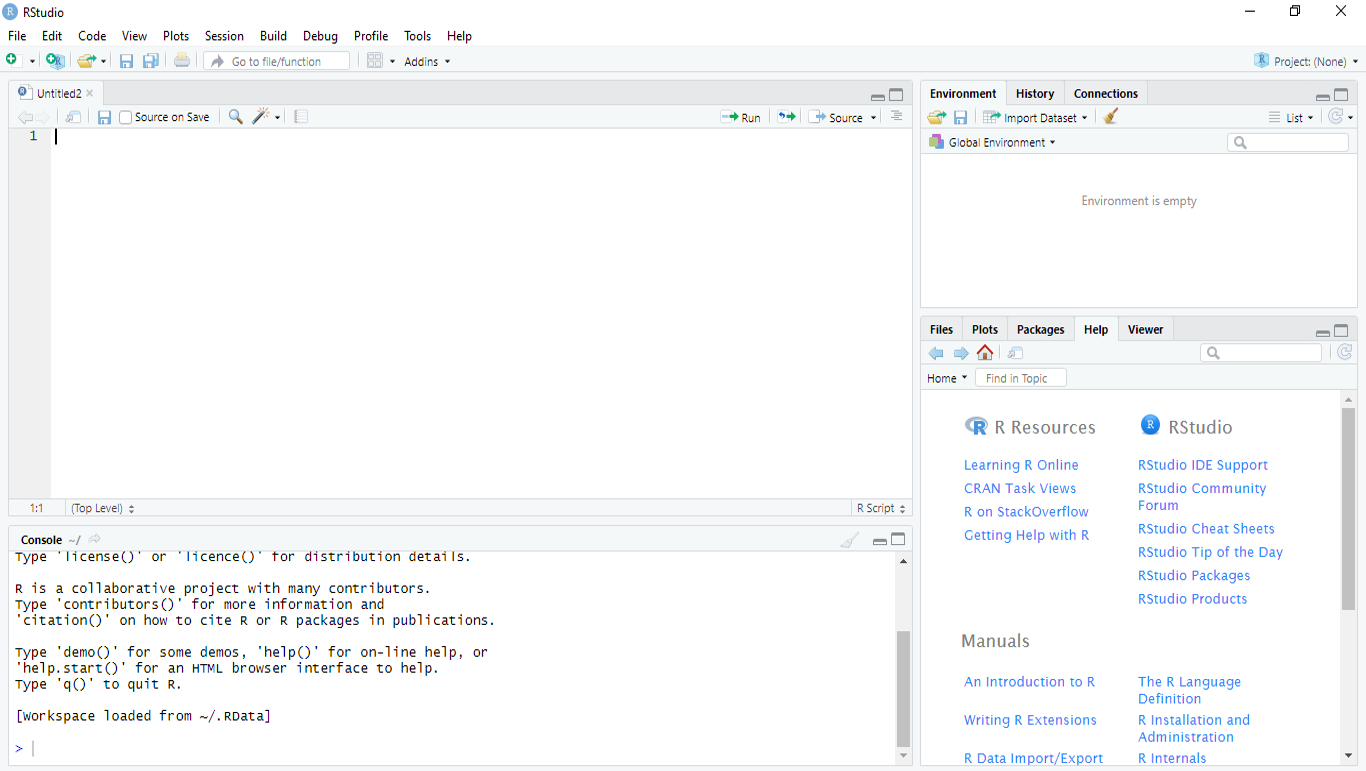
\includegraphics[width=1.1\linewidth]{/media/wilson/personaldoc/Livro_R/Série estatística passo a passo em excel e R/livroR-1.0/figures print/RStudio} 

}

\caption{Ambiente RStudio.}\label{fig:RStudio}
\end{figure}

O primeiro passo para que possamos compreender o R e o RStudio e o que podemos fazer com ele consiste em entender a sua estrutura como ela está organizada e o que ela significa. Uma vez compreendida sua estrutura organizacional e funcionalidade poderemos mergulhar no mundo das análises de dados dentro deste novo ambiente.

Para isso veremos as principais guias do RStudio, como elas estão organizadas e quais as suas principais funcionalidades.

\begin{enumerate}
\def\labelenumi{\arabic{enumi}.}
\tightlist
\item
  \emph{Script}: Guia utilizada para escrevermos o nosso código (comandos que executarão uma determinada tarefa) e comentários. Para executar os comandos escritos neste ambiente devemos deixar o cursor na linha que queremos executar e utilizar os atalhos do teclado \((CTRL + ENTER)\) ou \((CTRL + R)\) ou clicar em ``\textbf{Run}'' (Figura \ref{fig:script}). Todo comando executado irá retornar uma saída na guia do ``\emph{console}'' (ver item 2). Se o comando executado indicar que o resultado será guardado em um objeto\footnote{Há diferentes tipos de objetos no R, falaremos sobre eles no próximo capítulo.}, este irá aparecer na guia ``\emph{environment}'' (ver item 3). Para salvar o script escrito você deve utilizar a opção \emph{File} na ``barra de menus'' e clicar em \emph{Save} ou usar o atalho \((CTRL + S)\) ou clicar no icone de ``disquete'' no canto superior esquerdo desta guia;
\end{enumerate}

\begin{figure}[H]

{\centering 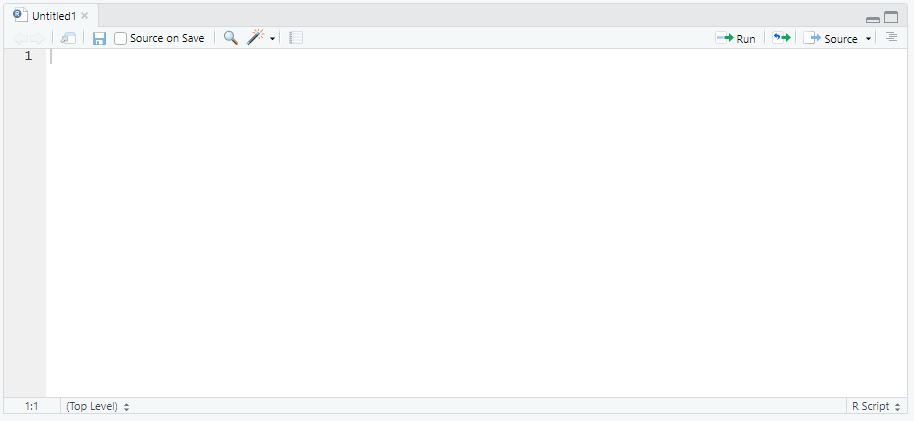
\includegraphics[width=1\linewidth]{/media/wilson/personaldoc/Livro_R/Série estatística passo a passo em excel e R/livroR-1.0/figures print/script} 

}

\caption{Guia do RStudio referente ao ambiente onde o script será desenvolvido.}\label{fig:script}
\end{figure}

\begin{enumerate}
\def\labelenumi{\arabic{enumi}.}
\setcounter{enumi}{1}
\tightlist
\item
  \emph{Console}: Guia que indica o resultado do código executado na guia referente ao \emph{script}. Nesta guia também pode ser escrito o código, porém ao pressionar ENTER o código é executado e o resultado é indicado na linha imediatamente inferior (Figura \ref{fig:console});
\end{enumerate}

\begin{figure}[H]

{\centering 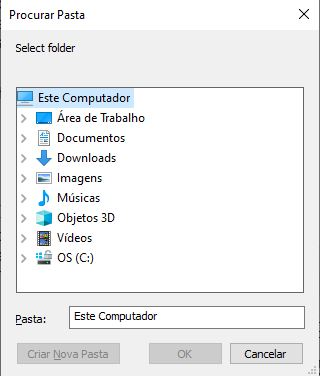
\includegraphics[width=1\linewidth]{/media/wilson/personaldoc/Livro_R/Série estatística passo a passo em excel e R/livroR-1.0/figures print/console} 

}

\caption{Guia do RStudio referente ao ambiente console onde o resultado dos comandos executados irão aparecer.}\label{fig:console}
\end{figure}

\begin{enumerate}
\def\labelenumi{\arabic{enumi}.}
\setcounter{enumi}{2}
\tightlist
\item
  \emph{Environment}: Todo objeto\footnote{Elemento que armazena um valor ou estrutura de dados. Todo objeto apresenta uma classe. Os objetos mais comuns são: vetor (objeto que contêm uma sequência unidimensional de elementos), matriz (Objeto bidimensional onde todos os elementos são da mesma classe), data-frame (Objeto bidimensional onde os elementos pertencentes podem ser de classes diferentes) e lista (é um vetor que agrupa, de maneira unidimensional, diferentes objetos). As classes mais comuns são: inteiro (valores quantitativos sem casa decimal), númerico (valores quantitativos com casa decimal), lógico (valores que indicam 0 ou 1, que representam respectivamente verdadeiro ou falso), fator (valores que indicam categorias) e caracter (valores que indicam texto). Vamos utiliza-los sempre que necessário, no decorrer do livro explicando-o seu significado, porém não iremos abordá-los em detalhes.} ou função criada será indicado nesta guia. (Figura \ref{fig:environment});
\end{enumerate}

\begin{figure}[H]

{\centering 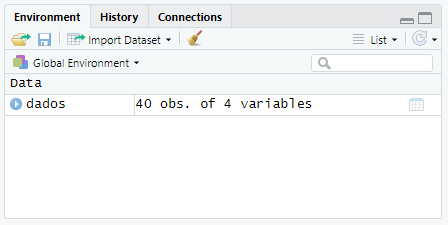
\includegraphics[width=0.6\linewidth]{/media/wilson/personaldoc/Livro_R/Série estatística passo a passo em excel e R/livroR-1.0/figures print/environment} 

}

\caption{Guia do RStudio referente ao ambiente environment, local onde estarão indicados os objetos criados.}\label{fig:environment}
\end{figure}

\begin{enumerate}
\def\labelenumi{\arabic{enumi}.}
\setcounter{enumi}{3}
\tightlist
\item
  \emph{History}: Guia que indica o histórico dos comandos executados (Figura \ref{fig:history});
\end{enumerate}

\begin{figure}[H]

{\centering 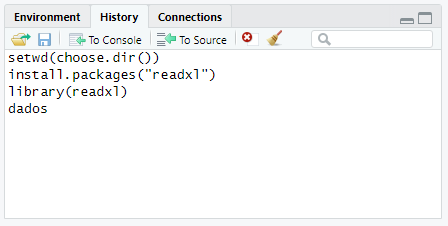
\includegraphics[width=0.6\linewidth]{/media/wilson/personaldoc/Livro_R/Série estatística passo a passo em excel e R/livroR-1.0/figures print/history} 

}

\caption{Guia do RStudio referente ao ambiente history onde estará listado todos os comandos executados.}\label{fig:history}
\end{figure}

\begin{enumerate}
\def\labelenumi{\arabic{enumi}.}
\setcounter{enumi}{4}
\tightlist
\item
  \emph{Files}: Guia que permite a visualização e acesso dos arquivos do computador (Figura \ref{fig:files}). Sempre defina o ambiente de trabalho\footnote{No próximo capítulo ensinaremos a como definir o ambiente de trabalho} antes de iniciar o seu projeto. As planilhas que serão utilizadas devem estar neste ambiente de trabalho, previamente definido. Embora não seja obrigatório, isso evitará problemas futuros e facilitará o seu trajeto inicial no R. As funções e códigos serão abordados, aqui, seguindo esta ideia.;
\end{enumerate}

\begin{figure}[H]

{\centering 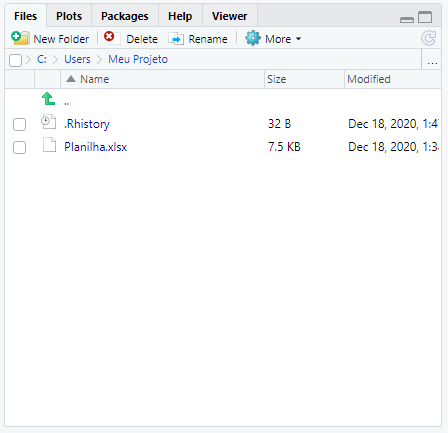
\includegraphics[width=0.6\linewidth]{/media/wilson/personaldoc/Livro_R/Série estatística passo a passo em excel e R/livroR-1.0/figures print/files} 

}

\caption{Guia do RStudio referente ao ambiente files onde estará indicados os arquivos do nosso computador.}\label{fig:files}
\end{figure}

\begin{enumerate}
\def\labelenumi{\arabic{enumi}.}
\setcounter{enumi}{5}
\tightlist
\item
  \emph{Packages}: Guia destinada a visualização, instalação e carregamento dos pacotes/bibliotecas do R. Os pacotes consistem em um grupo de funções, que executam uma determinada ação. Inicialmente quando se instala o R alguns pacotes são automaticamente instalados. Contudo para executar algumas funções é necessário instalar um ou mais pacotes que contenham as funções desejadas. A instalação de pacotes pode ser realizada por linha de comando como será visto no próximo capítulo ou clicando na opção \emph{Install} presente no canto superior esquerdo desta guia. De tempos em tempos os pacotes sofrem alterações, realizado pelos seus desenvolvedores, por isso um hábito importante a ser tomado de tempos em tempos é clicar na opção \emph{Update} ao lado da opção \emph{Install} pois ela irá atualizar os pacotes que estão instalados (Figura \ref{fig:packages});
\end{enumerate}

\begin{figure}[H]

{\centering 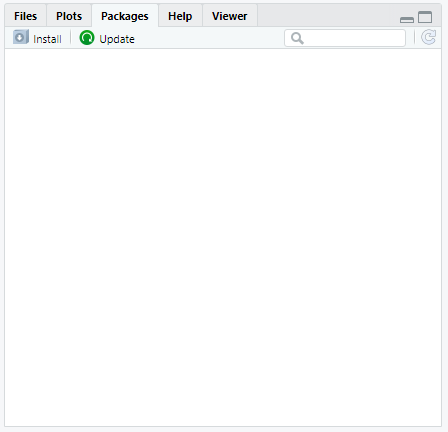
\includegraphics[width=0.6\linewidth]{/media/wilson/personaldoc/Livro_R/Série estatística passo a passo em excel e R/livroR-1.0/figures print/packages} 

}

\caption{Guia do RStudio referente ao ambiente packages onde estarão listados todos os pacotes disponíveis no nosso computador e por onde poderemos instalar outros.}\label{fig:packages}
\end{figure}

\begin{enumerate}
\def\labelenumi{\arabic{enumi}.}
\setcounter{enumi}{6}
\tightlist
\item
  \emph{Plot}: Guia destinada a visualização dos gráficos executados. Algumas opções importantes desta guia é a opção \emph{Export} na região central na barra de ferramentas onde é possível salvar o seu plot como imagem em formato *.jpg, *.png e *.tiff, por exemplo, assim como em *.pdf ou então a opção de copiar a imagem (\emph{Copy to Clipboard\ldots{}}) para colar em outro ambiente de trabalho. Uma segunda ferramenta importante é a opção do lado direito de \emph{Export} que é \emph{Remove the current plot} indicada por um quadrado branco com um ``x'' branco de fundo vermelho no canto superior esquerdo o qual remove a figura que está sendo visualizada neste ambiente, ao lado desta opção tem a figura de uma vassoura denominada \emph{Clear all Plots} que deleta todas as figuras presentes neste ambiente. No lado esquerdo de \emph{Export} temos a opção de \emph{Zoom} o qual amplia a imagem mostrada e ao lado esquerdo desta opção temos setas indicando para direita e para esquerda, que permitem navegar por entre os plots criados durante seu trabalho (Figura \ref{fig:plot});
\end{enumerate}

\begin{figure}[H]

{\centering 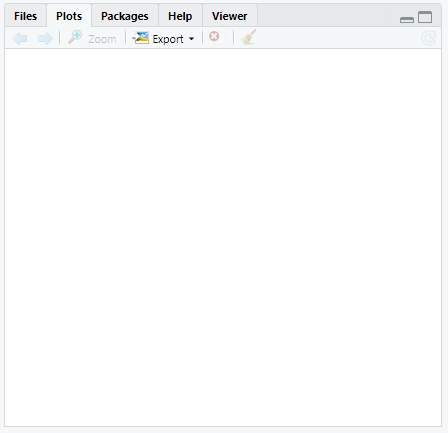
\includegraphics[width=0.6\linewidth]{/media/wilson/personaldoc/Livro_R/Série estatística passo a passo em excel e R/livroR-1.0/figures print/plot} 

}

\caption{Guia do RStudio referente ao ambiente plot onde estarão os gráficos criados.}\label{fig:plot}
\end{figure}

\begin{enumerate}
\def\labelenumi{\arabic{enumi}.}
\setcounter{enumi}{7}
\tightlist
\item
  \emph{Help}: Guia destinada a fornecer informações sobre as funções e pacotes do R. Nesta guia há duas opções importantes na sua barra superior uma encontra-se na barra mais superior indicada por uma lupa onde é possível digitar o nome do pacote ou função em que deseja saber mais sobre, na barra abaixo desta no canto esquerdo há um outro espaço escrito \emph{Find in Topic} onde ele irá buscar o termo digitado dentro do ambiente que está sendo mostrado (Figura \ref{fig:help});
\end{enumerate}

\begin{figure}[H]

{\centering 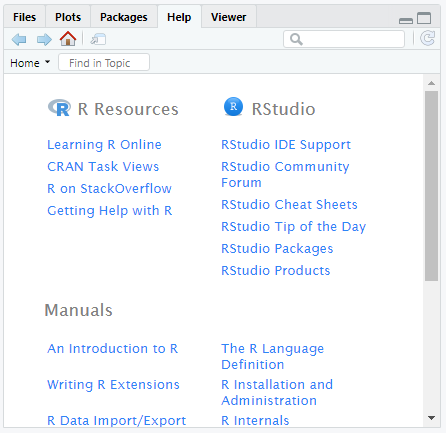
\includegraphics[width=0.6\linewidth]{/media/wilson/personaldoc/Livro_R/Série estatística passo a passo em excel e R/livroR-1.0/figures print/help} 

}

\caption{Guia do RStudio referente ao ambiente help onde terá informações sobre as funções e pacotes do R.}\label{fig:help}
\end{figure}

\hypertarget{exercuxedcios}{%
\section{Exercícios}\label{exercuxedcios}}

\begin{enumerate}
\def\labelenumi{\arabic{enumi})}
\tightlist
\item
  Após escrever um comando na guia \emph{script}, como fazemos para executa-lo?
\end{enumerate}

\begin{enumerate}
\def\labelenumi{(\alph{enumi})}
\tightlist
\item
  Pressionamos a tecla ENTER
\item
  Pressionamos as teclas CTRL + ENTER
\item
  Pressionamos as teclas CTRL + SPACE
\item
  Pressionamos as teclas SHIFT + ENTER
\item
  Presionamos as teclas CTRL + SHIFT + ENTER
\end{enumerate}

\begin{enumerate}
\def\labelenumi{\arabic{enumi})}
\setcounter{enumi}{1}
\tightlist
\item
  Após escrevermos um comando na guia \emph{console}, como fazemos para executa-lo?
\end{enumerate}

\begin{enumerate}
\def\labelenumi{(\alph{enumi})}
\tightlist
\item
  Pressionamos a tecla ENTER
\item
  Pressionamos as teclas CTRL + S
\item
  Pressionamos as teclas CTRL + SPACE
\item
  Pressionamos as teclas SHIFT + ENTER
\item
  Presionamos as teclas CTRL + SHIFT + ENTER
\end{enumerate}

\begin{enumerate}
\def\labelenumi{\arabic{enumi})}
\setcounter{enumi}{2}
\tightlist
\item
  Ao realizarmos um gráfico, em que guia ele irá aparecer
\end{enumerate}

\begin{enumerate}
\def\labelenumi{(\alph{enumi})}
\tightlist
\item
  \emph{console}
\item
  \emph{Viewer}
\item
  \emph{Plots}
\item
  \emph{Environment}
\item
  \emph{Script}
\end{enumerate}

\begin{enumerate}
\def\labelenumi{\arabic{enumi})}
\setcounter{enumi}{3}
\tightlist
\item
  Se desejarmos verificar os comandos previamente executados, mesmo após ter reiniciado o R, qual é a melhor forma de consulta?
\end{enumerate}

\begin{enumerate}
\def\labelenumi{(\alph{enumi})}
\tightlist
\item
  Verificar o \emph{console}
\item
  Acessar a guia \emph{history}
\item
  Acessar a guia \emph{environment}
\item
  Verificar o \emph{script}
\item
  Acessar a guia \emph{help}
\end{enumerate}

\begin{enumerate}
\def\labelenumi{\arabic{enumi})}
\setcounter{enumi}{4}
\tightlist
\item
  Se executarmos um comando na guia \emph{script}, em que guia o resultado irá aparecer?
\end{enumerate}

\begin{enumerate}
\def\labelenumi{(\alph{enumi})}
\tightlist
\item
  Obrigatoriamente nas guias \emph{console} e \emph{environment}
\item
  Obrigatoriamente nas guias \emph{plots} e \emph{console}
\item
  Obrigatoriamente na guia \emph{environment}
\item
  Obrigatoriamente nas guias \emph{plots} e \emph{environment}
\item
  Obrigatoriamente na guia \emph{console}
\end{enumerate}

\hypertarget{importar-organizar-e-sumarizar-os-dados}{%
\chapter{Importar, organizar e sumarizar os dados}\label{importar-organizar-e-sumarizar-os-dados}}

\hypertarget{passo-definir-o-ambiente-de-trabalho-e-importar-a-planilha-de-dados-para-o-r}{%
\section{1° passo: Definir o ambiente de trabalho e importar a planilha de dados para o R}\label{passo-definir-o-ambiente-de-trabalho-e-importar-a-planilha-de-dados-para-o-r}}

Ao se trabalhar com R a primeira pergunta que nos vem à cabeça é: Como inserir meus dados neste ambiente de trabalho? A resposta é simples e também complexa, pois depende do formato do arquivo de dados que está usando ( *.csv, *.xls, *.xlsx, *.txt entre outros). Para um mesmo formato existem inúmeras comandos possíveis para importar os dados. Não iremos especificar todas os comandos, mas os mais comuns (*.csv e *.xlsx), utilizando os comandos básicos do R e também por meio da interface gráfica do RStudio.

Para importar a planilha é necessário definir o ambiente de trabalho no seu computador. Este ambiente é a pasta de seu computador onde sua planilha e seus demais dados a serem trabalhados se encontram. Podemos realizar isso via linhas de comando ou pela própria interface do RStudio. Se realizado por linhas de comandos há diferença entre o sistema operacional (Windows, Linux ou macOS) que estiver utilizando. Aqui estaremos trabalhando com o sistema operacional Windows.

\hypertarget{definindo-ambiente-de-trabalho-via-linha-de-comando}{%
\subsection{Definindo ambiente de trabalho via linha de comando}\label{definindo-ambiente-de-trabalho-via-linha-de-comando}}

Para o sistema operacional Windows utilizamos o seguinte comando: \textcolor{blue}{setwd(choose.dir(path))}, onde \textcolor{blue}{path} é o caminho do diretório escolhido.

Se no Windows utilizarmos apenas a linha de comando \textcolor{blue}{setwd(choose.dir())} sem especificar o caminho a seguinte janela irá aparecer (Figura \ref{fig:setwd}), a partir da qual iremos selecionar a pasta onde estão os arquivos que iremos trabalhar e salvar nosso \emph{script}.

\begin{figure}[H]

{\centering 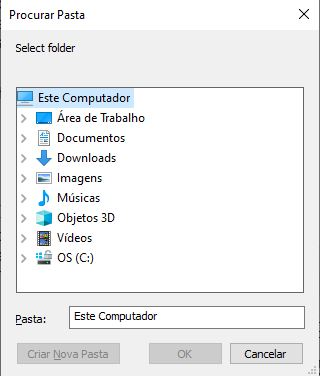
\includegraphics[width=0.4\linewidth]{/media/wilson/personaldoc/Livro_R/Série estatística passo a passo em excel e R/livroR-1.0/figures print/setwd} 

}

\caption{Janela que será aberta ao executar o comando: setwd(choose.dir()), no sistema operacional Windows.}\label{fig:setwd}
\end{figure}

A função \textcolor{blue}{setwd()} é responsável por selecionar o diretório a ser trabalhado. Após isso podemos importar a planilha com os dados que utilizaremos.

Como resultado desta etapa podemos verificar a guia \emph{Files}\footnote{Ver figura \ref{fig:files}}, nela agora situa-se as pastas e arquivos da pasta que selecionamos e onde estará salvo nosso script quando o salvarmos.

\hypertarget{definindo-ambiente-de-trabalho-via-interface-gruxe1fica}{%
\subsection{Definindo ambiente de trabalho via interface gráfica}\label{definindo-ambiente-de-trabalho-via-interface-gruxe1fica}}

Diversas formas podem ser utilizadas para definir o ambiente de trabalho, apresentaremos 3. A primeira consiste em usar o atalho do teclado \((CTRL + SHIFT + H)\) e nela selecionaremos o ambiente de trabalho; a segunda via consiste em acessar a guia \emph{Session} ir até a opção \emph{Set Working Directory} e selecionar a opção \emph{Choose Directory} da mesma forma que a opção anterior a mesma janela irá aparecer; por último podemos usar a guia \emph{Files} onde podemos clicar nos 3 pontos ``\ldots{}'' que aparecem no canto superior direito da guia e buscar o ambiente/pasta que iremos utilizar e a seguir na engrenagem (\emph{More}) e selecionar a opção \emph{Set as Working Directory} (Figura \ref{fig:files-guia}).

\begin{figure}[H]

{\centering 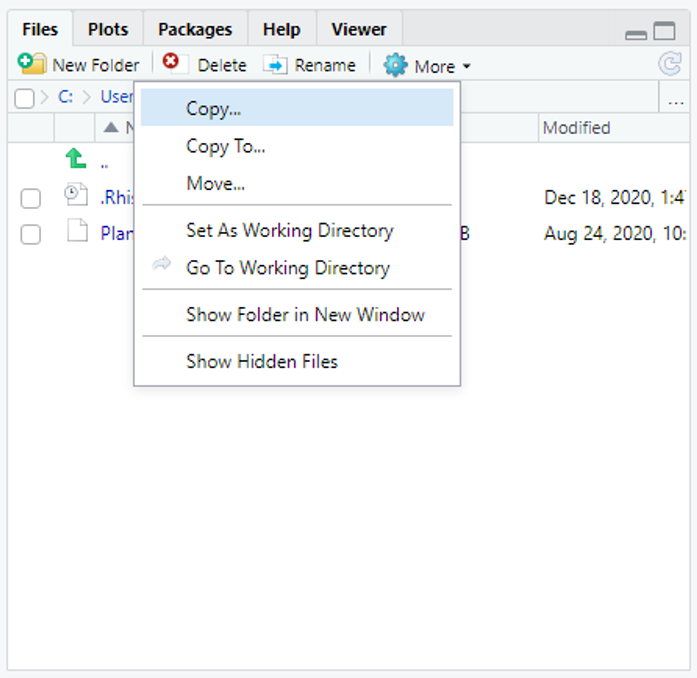
\includegraphics[width=0.5\linewidth]{/media/wilson/personaldoc/Livro_R/Série estatística passo a passo em excel e R/livroR-1.0/figures print/files-guia} 

}

\caption{Guia *Files* indicando a opção para definir o local do computadors que será utilizado como ambiente de trabalho}\label{fig:files-guia}
\end{figure}

\hypertarget{importando-planilha-via-linha-de-comando}{%
\subsection{Importando planilha via linha de comando:}\label{importando-planilha-via-linha-de-comando}}

Primeiro construa as planilhas a seguir nos formatos *.csv (usando vírgula como separador de colunas e ponto como separador decimal) (Figura \ref{fig:planilha}) e *.xlsx (Figura \ref{fig:planilhaxlsx}) em um editor de planilhas, como excel, libreoffice calc ou outros e a salve com o nome de planilha.csv e planilha.xlsx no diretório que definiu previamente. A seguir demonstraremos as diferenças na importação de ambas as planilhas.

\begin{figure}[H]

{\centering 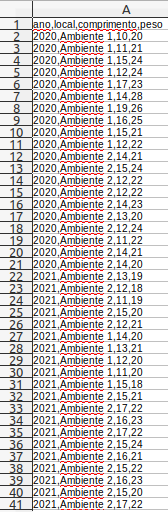
\includegraphics[width=0.4\linewidth]{/media/wilson/personaldoc/Livro_R/Série estatística passo a passo em excel e R/livroR-1.0/figures print/planilha} 

}

\caption{Planilha com os dados no formato *.csv que deve ser construída em algum editor de planilhas e salva na pasta de trabalho definida previamente}\label{fig:planilha}
\end{figure}

\begin{figure}[H]

{\centering 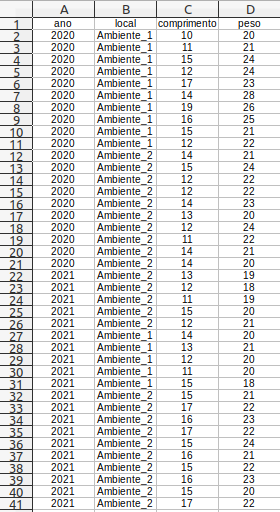
\includegraphics[width=0.5\linewidth]{/media/wilson/personaldoc/Livro_R/Série estatística passo a passo em excel e R/livroR-1.0/figures print/planilhaxlsx} 

}

\caption{Planilha com os dados no formato *.xlsx que deve ser construída em algum editor de planilhas e salva na pasta de trabalho definida previamente}\label{fig:planilhaxlsx}
\end{figure}

Digite em seu script a seguinte linha de comando:

\begin{Shaded}
\begin{Highlighting}[]
\NormalTok{dados <-}\StringTok{ }\KeywordTok{read.csv}\NormalTok{(}\DataTypeTok{file =} \StringTok{"planilha.csv"}\NormalTok{, }\DataTypeTok{header =} \OtherTok{TRUE}\NormalTok{, }\DataTypeTok{sep =} \StringTok{","}\NormalTok{)}
\end{Highlighting}
\end{Shaded}

\textcolor{red}{OBS: Não se esqueça de definir previamente o ambiente de trabalho e verificar que o arquivo planilha.csv encontra-se presente nele.}

O comando \textcolor{blue}{read.csv()} importou a planilha que está no formato *.csv utilizando os argumentos ``\emph{file}'' o qual indica o nome do arquivo a ser importado; ``\emph{header}'' o qual indica se as colunas da planilha tem nome e ``sep'' o qual indica qual o caracter separador das colunas.

\textcolor{red}{OBS: repare que há o operador} ``\textbf{\textless{}-}'' \textcolor{red}{, esse é o operador de atribuição, ele indica que o elemento a sua direita (seja um valor ou uma função) será atribuído ao elemento que está a sua esquerda (geralmente um novo objeto). Neste caso o elemento retornado pela função } read.csv(file = ``planilha.csv'', header = TRUE, sep = ``,'') \textcolor{red}{ será atribuído a um objeto chamado **dados**.}

O comando acima importou a planilha e o guardou em um objeto chamado dados que será o que nós utilizaremos de agora em diante sempre que quisermos acessar essa planilha no RStudio.

Para importar arquivos que estão no formato *.xls ou *.xlsx é necessário a instalação de algum pacote\footnote{Tudo que é realizado no R é por meio de comandos, esses comandos são compostos de funções, podemos reconhece-las pois logo após um nome que representa uma função obrigatoriamente há um parênteses e cada função apresenta argumentos, depois dos quais há o sinal de igual (=). As funções estão dentro de pacotes/bibliotecas, ou seja, cada biblioteca apresenta diversas funções e cada função diversos argumentos. O R, quando instalado, traz consigo alguns pacotes, mas estes pacotes não apresentam uma função que permite carregar arquivos *.xls ou *.xlsx. Portanto para que seja possível realizar essa tarefa devemos instalar, neste caso, o pacote readxl. Para instalação de pacotes podemos usar a função conhecida por install.packages(``nome do pacote'').} que permita a realização desse processo. Um pacote que instalaremos aqui é o \textcolor{brown}{readxl}.

\begin{Shaded}
\begin{Highlighting}[]
\KeywordTok{install.packages}\NormalTok{(}\StringTok{"readxl"}\NormalTok{)}
\KeywordTok{library}\NormalTok{(readxl)}
\end{Highlighting}
\end{Shaded}

\begin{Shaded}
\begin{Highlighting}[]
\NormalTok{dados <-}\StringTok{ }\KeywordTok{read_excel}\NormalTok{(}\DataTypeTok{path =} \StringTok{"planilha.xlsx"}\NormalTok{, }\DataTypeTok{col_names =} \OtherTok{TRUE}\NormalTok{)}
\end{Highlighting}
\end{Shaded}

Os comandos \textcolor{blue}{read.csv()} e \textcolor{blue}{read\_excel()} são similares, embora seus argumentos sejam diferentes. O argumento ``\emph{path}'' é similar ao ``\emph{file}'', o argumento ``\emph{col\_names}'' é similar ao ``\emph{header}''. Repare que não temos o argumento ``sep'', pois em um arquivo excel as variáveis são salvas em colunas. Observe que independente da forma de importação (que é dependente do formato do arquivo *.csv ou *.xlsx) o resultado final é o mesmo (Figura \ref{fig:arqenv}).

\begin{figure}[H]

{\centering 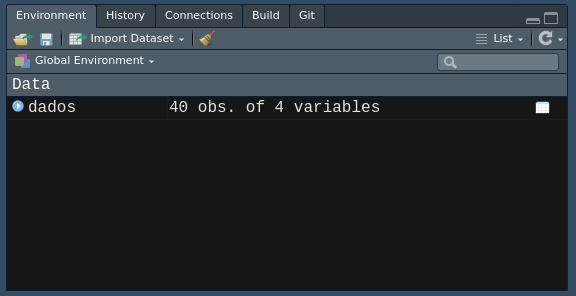
\includegraphics[width=0.8\linewidth]{/media/wilson/personaldoc/Livro_R/Série estatística passo a passo em excel e R/livroR-1.0/figures print/arqenv} 

}

\caption{Resultado da importação do arquivo observado na guia environment. Há um objeto de nome dados, com 40 observações e 4 variáveis.}\label{fig:arqenv}
\end{figure}

\hypertarget{importando-planilha-via-interface-gruxe1fica}{%
\subsection{Importando planilha via interface gráfica:}\label{importando-planilha-via-interface-gruxe1fica}}

Para importar a planilha com os dados via interface do RStudio devemos acessar a guia \emph{Environment} e nesta acessar a opção \emph{Import Dataset} a seguir temos várias opções a qual devemos escolher referente a extensão do arquivo que vamos importar, no nosso caso será a opção \emph{From Excel} (Figura \ref{fig:import-graf}).

\begin{figure}[H]

{\centering 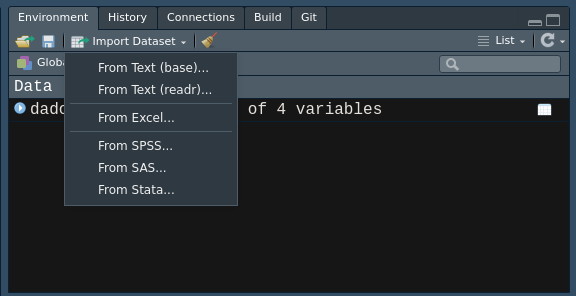
\includegraphics[width=0.8\linewidth]{/media/wilson/personaldoc/Livro_R/Série estatística passo a passo em excel e R/livroR-1.0/figures print/import-graf} 

}

\caption{Tópicos para importação ddos dados pela via grafica.}\label{fig:import-graf}
\end{figure}

Neste momento uma janela irá abrir (Figura \ref{fig:import-graf-2}) e no canto superior direito haverá o nome \emph{Browse} onde deveremos clicar e escolher o arquivo com o qual iremos trabalhar. Em \emph{Import options} no canto inferior esquerdo haverá algumas opções, na opção \emph{name} deveremos renomear para dados, para coincidir com as vias que fizemos anteriormente. As demais opções podemos deixar em branco. Repare que no canto inferior direito aparecerá um comando relativo ao processo de importação similar ao que fizemos no tópico anterior e, aparecerá também, um comando chamado \textcolor{blue}{View()} que veremos mais adiante, para desabilita-lo basta desmarcar a caixa ao lado de mesmo nome. Conclua o processo clicando em \emph{import} no canto inferior direito.

\begin{figure}[H]

{\centering 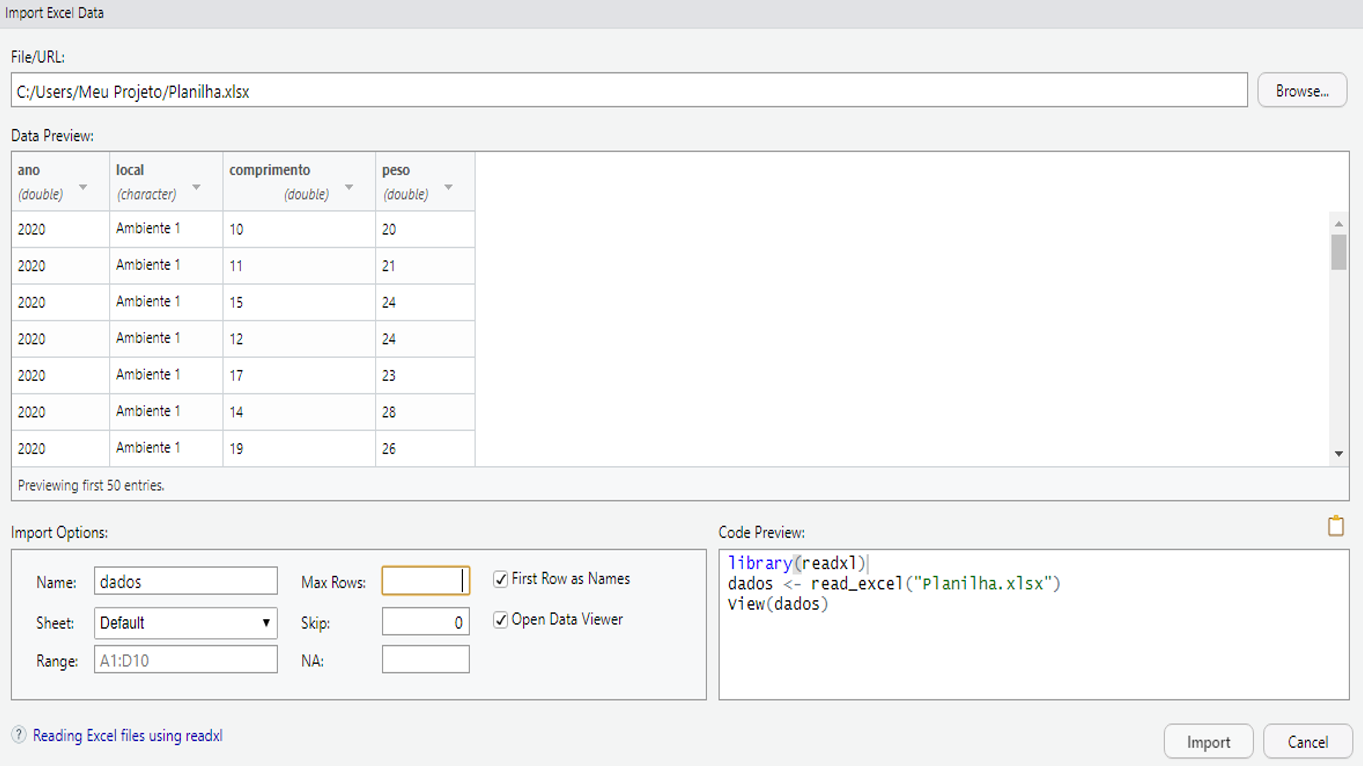
\includegraphics[width=0.8\linewidth]{/media/wilson/personaldoc/Livro_R/Série estatística passo a passo em excel e R/livroR-1.0/figures print/import-graf-2} 

}

\caption{Importação dos dados pela via gráfica}\label{fig:import-graf-2}
\end{figure}

\hypertarget{passo-verificar-e-ajustar-os-dados}{%
\section{2° passo: Verificar e ajustar os dados}\label{passo-verificar-e-ajustar-os-dados}}

Uma falha inicial comum é passar para as análises antes de verificar se os dados estão corretamente organizados, após a importação. Uma forma de previnir isso é conhecendo os seus dados e sabendo o que eles significam. Os dados, geralmente, podem ser: categóricos (ou qualitativos) ou mensuráveis (ou quantitativos). Quando categóricos temos de informar que eles consistem em fatores. Para isso vamos executar alguns comandos onde poderemos avaliar se no processo de importação as variáveis presentes na planilha de dados são reconhecidas como esperamos que seja.

Ao executarmos a função \textcolor{blue}{str()} do arquivo \textbf{dados} podemos ver no console o seguinte resultado

\begin{Shaded}
\begin{Highlighting}[]
\KeywordTok{str}\NormalTok{(dados)}
\end{Highlighting}
\end{Shaded}

\begin{verbatim}
## tibble[,4] [40 x 4] (S3: tbl_df/tbl/data.frame)
##  $ ano        : num [1:40] 2020 2020 2020 2020 2020 2020 2020 2020 2020 2020 ...
##  $ local      : chr [1:40] "Ambiente 1" "Ambiente 1" "Ambiente 1" "Ambiente 1" ...
##  $ comprimento: num [1:40] 10 11 15 12 17 14 19 16 15 12 ...
##  $ peso       : num [1:40] 20 21 24 24 23 28 26 25 21 22 ...
\end{verbatim}

Seu resultado nos informa sobre o tipo de objeto que o arquivo é. Todo objeto pertence a alguma classe neste caso nosso objeto e da classe \emph{tibble} ou \emph{data frame}\footnote{tibble e data frame são, em termos práticos para o livro, objetos similares}.

Também nos é mostrado as variáveis presentes na planilha \textbf{dados} (ano, local, comprimento e peso), cada variável é, também, um objeto e portanto tem suas classes definidas automaticamente, o que pode ser visualizado ao lado de cada variável.

num = \emph{numeric} (númerico), chr = \emph{character} (caracter) e há outras que não estão indicadas aqui, como \emph{logic} (lógica), \emph{integer} (inteiro), \emph{factor} (fator) entre outros.

Repare que a variável ano foi indicada como numérico. Variáveis consideradas numéricas são aquelas as quais foram mensuradas. Ano, embora númerica, não é uma variável possível de ser medida, porém devido ao seu registro ter sido em valores numéricos foi assim que ela foi entendida. Portanto temos que transforma-la.

Pensando no que definimos acima com variáveis categóricas e mensuráveis, ano e local podem ser classificados como variáveis categóricas. Devemos transformar em fator todas as variáveis de nossas planilha consideradas categóricas. Para isso utilizamos a função \textcolor{blue}{as.factor()} a qual realiza esse processo que pode ser feito da seguinte forma:

\begin{Shaded}
\begin{Highlighting}[]
\NormalTok{dados}\OperatorTok{$}\NormalTok{ano <-}\StringTok{ }\KeywordTok{as.factor}\NormalTok{(dados}\OperatorTok{$}\NormalTok{ano)}
\NormalTok{dados}\OperatorTok{$}\NormalTok{local <-}\StringTok{ }\KeywordTok{as.factor}\NormalTok{(dados}\OperatorTok{$}\NormalTok{local)}
\end{Highlighting}
\end{Shaded}

Repare que nesses comandos inserimos o operador ``\textbf{\$}'' (cifrão). Esse é um operador importante em toda linguagem de programação e será bastante utilizado. Ele permite acessar alguma variável dentro de um objeto. Pensando no objeto \textbf{dados}, ao colocarmos seu nome e em seguida o operador ``\textbf{\$}'' podemos acessar as variáveis dentro dele.

O comando portanto é lido da seguinte forma:

\begin{enumerate}
\def\labelenumi{\arabic{enumi}.}
\tightlist
\item
  dados\$ano \textless{}-: indica que uma variável ano será criada dentro do objeto \textbf{dados}.
\item
  as.factor(dados\$ano): indica que o objeto criado consistirá na variável ano que está no objeto dados porém considerando-a como factor.
\end{enumerate}

Uma dúvida que pode aparecer aqui é: O que aconteceu com a variável ano que já existia dentro da planilha dados? Temos duas variáveis ano, agora?

A resposta é que quando criamos um objeto ou variável com o mesmo nome de um já existente o anterior é substituído. Conduza o seguinte exemplo.

Crie o objeto \textbf{idade} que contenha o valor de 30.

\begin{Shaded}
\begin{Highlighting}[]
\NormalTok{idade <-}\StringTok{ }\DecValTok{30}
\end{Highlighting}
\end{Shaded}

Repare o objeto idade criado no \emph{environment}.

Agora crie e execute um segundo objeto de mesmo nome, porém valor diferente, e repare no \emph{enviroment}.

\begin{Shaded}
\begin{Highlighting}[]
\NormalTok{idade <-}\StringTok{ }\DecValTok{40}
\end{Highlighting}
\end{Shaded}

Reparou que ao criar um segundo objeto de mesmo nome que antes o primeiro foi apagado e substituído pelo segundo? Este é o mesmo processo que ocorreu quando realizamos a função que definiu ano e local como fatores dentro do objeto \textbf{dados}.

Vamos observar novamente a função \textcolor{blue}{str()} para verificar se ano e locais, agora, são fatores

\begin{Shaded}
\begin{Highlighting}[]
\KeywordTok{str}\NormalTok{(dados)}
\end{Highlighting}
\end{Shaded}

\begin{verbatim}
## tibble[,4] [40 x 4] (S3: tbl_df/tbl/data.frame)
##  $ ano        : Factor w/ 2 levels "2020","2021": 1 1 1 1 1 1 1 1 1 1 ...
##  $ local      : Factor w/ 2 levels "Ambiente 1","Ambiente 2": 1 1 1 1 1 1 1 1 1 1 ...
##  $ comprimento: num [1:40] 10 11 15 12 17 14 19 16 15 12 ...
##  $ peso       : num [1:40] 20 21 24 24 23 28 26 25 21 22 ...
\end{verbatim}

Como pode verificar agora temos 2 variáveis como fatores e 2 como numéricas. Mais que isso, essa função nos indica ao lado dos fatores um \emph{w/2 levels} que está nos dizendo que essa variável tem 2 níveis. De maneira similar, as variáveis numéricas indicam colchetes com os seguintes valores {[}1:40{]} que significa que temos 40 valores/observações/linhas.

Observe a planilha dados no environment. Note que ao lado do nome dados há escrito \textbf{40obs. of 4 variables}. Isto indica que temos 40 observações e 4 variáveis.

Que tal agora observarmos nossa planilha? Podemos fazer isso por meio da execução função \textcolor{blue}{head()} do nosso objeto (\textbf{dados}). Onde no console são mostradas as primeiras linhas de nossa planilha

\begin{Shaded}
\begin{Highlighting}[]
\KeywordTok{head}\NormalTok{(dados)}
\end{Highlighting}
\end{Shaded}

\begin{verbatim}
## # A tibble: 6 x 4
##   ano   local      comprimento  peso
##   <fct> <fct>            <dbl> <dbl>
## 1 2020  Ambiente 1          10    20
## 2 2020  Ambiente 1          11    21
## 3 2020  Ambiente 1          15    24
## 4 2020  Ambiente 1          12    24
## 5 2020  Ambiente 1          17    23
## 6 2020  Ambiente 1          14    28
\end{verbatim}

Outra maneira é executarmos a função \textcolor{blue}{View()} que abre uma aba, ao lado de seu script mostrando todos os dados.

\begin{Shaded}
\begin{Highlighting}[]
\KeywordTok{View}\NormalTok{(dados)}
\end{Highlighting}
\end{Shaded}

Experimente agora escrever o nome do objeto \textbf{dados} e executar, o que aparece? Experimente, também, clicar no nome do objeto \textbf{dados}, presente no \emph{environment}. O que você observou?

Se no primeiro caso você observou seu objeto aparecendo no console, parabéns você está indo no caminho certo. Se no segundo momento você observou que ao clicar sobre o nome dados ele executou a mesma coisa que a função \textcolor{blue}{View()} você está indo maravilhosamente bem. Continue assim!

Isto não é tudo, mas sim o necessário para começarmos a sumarizar os dados de maneira eficiente.

Não se esqueça que antes de trabalharmos nossos dados temos que entender o que eles são e a que eles se referem. A análise de dados sem prévio conhecimento sobre o que eles significam pode levar a interpretações errôneas, caso as análises realizadas indiquem algum resultado, ou a muita dor de cabeça, se algum comando para uma análise não funcionar como esperado.

Portanto sigam os passos precisamente, não pule etapas e busque diversificar a fonte do seu conhecimento. Pois o R é uma linguagem que como demonstramos até o momento há muitas vias possíveis de escrita para um mesmo objetivo e diferentes autores podem escrever de formas diferentes.

\hypertarget{passo-sumarizar-os-dados-graficamente}{%
\section{3° passo: Sumarizar os dados graficamente}\label{passo-sumarizar-os-dados-graficamente}}

Já importamos nossa planilha e já a ajustamos. Que tal começarmos a ver a ``mágica'' acontecer e graficarmos nossos dados?

Muitos gráficos podem ser realizados, mas lembre-se que há toda uma lógica por trás disso.

Pensando nos gráficos mais comuns e úteis para nosso dia-a-dia e que nos permitem sumarizar nossos dados, temos os histogramas, gráficos de barras, de pontos, de linhas e os boxplots. Vamos então começar com esses e com o objetivo inicial de sumarizar nossos dados.

\hypertarget{histograma}{%
\subsection{Histograma}\label{histograma}}

O histograma nos permite verificar a distribuição da frequência dos nossos dados. Por exemplo, imagine uma amostra com diversos indivíduos de um dado grupo. Caso queiramos representar as frequências relativas das diferentes faixas de peso deste grupo, podemos usar o histograma.

A função \textcolor{blue}{hist()} permite visualizar os valores da variável comprimento (Figura \ref{fig:comp-hist}). Vejamos o exemplo abaixo.

\begin{Shaded}
\begin{Highlighting}[]
\KeywordTok{hist}\NormalTok{(dados}\OperatorTok{$}\NormalTok{comprimento)}
\end{Highlighting}
\end{Shaded}

\begin{figure}[H]

{\centering 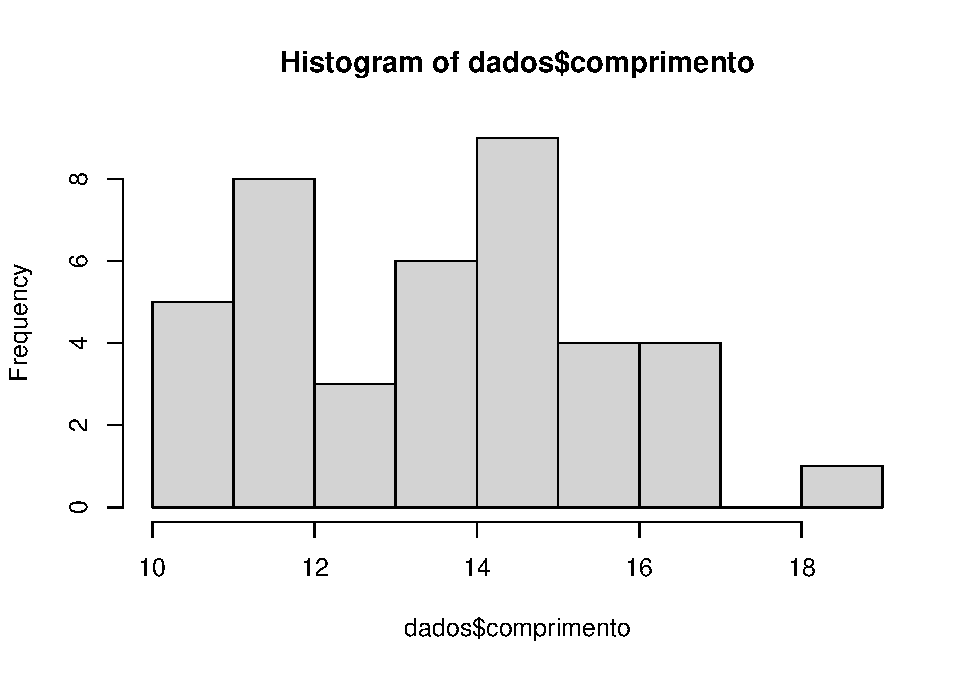
\includegraphics[width=0.7\linewidth]{livroR-1.0_files/figure-latex/comp-hist-1} 

}

\caption{Comprimento dos organismos da planilha dados}\label{fig:comp-hist}
\end{figure}

Repare que um gráfico foi gerado na sua janela lateral, na guia plots.

Perceba também que voltamos a usar o operador ``\textbf{\$}'' (cifrão).

Nosso gráfico não está com uma aparência muito agradável além de estar um pouco sem cor. Podemos editar e melhorar o aspecto do gráfico ao inserir cores ou outros argumentos estéticos que melhoram sua visualização e entender como ele sumariza nossos dados.

\begin{Shaded}
\begin{Highlighting}[]
\KeywordTok{hist}\NormalTok{(dados}\OperatorTok{$}\NormalTok{comprimento, }
     \DataTypeTok{ylim =} \KeywordTok{c}\NormalTok{(}\DecValTok{0}\NormalTok{, }\DecValTok{10}\NormalTok{), }
     \DataTypeTok{xlim =} \KeywordTok{c}\NormalTok{(}\DecValTok{9}\NormalTok{, }\DecValTok{20}\NormalTok{), }
     \DataTypeTok{col =} \StringTok{"blue"}\NormalTok{,}
     \DataTypeTok{main =} \StringTok{"Meu Histograma"}\NormalTok{,}
     \DataTypeTok{xlab =} \StringTok{"Comprimento"}\NormalTok{,}
     \DataTypeTok{ylab =} \StringTok{"Frequência absoluta"}\NormalTok{)}
\end{Highlighting}
\end{Shaded}

\begin{figure}[H]

{\centering 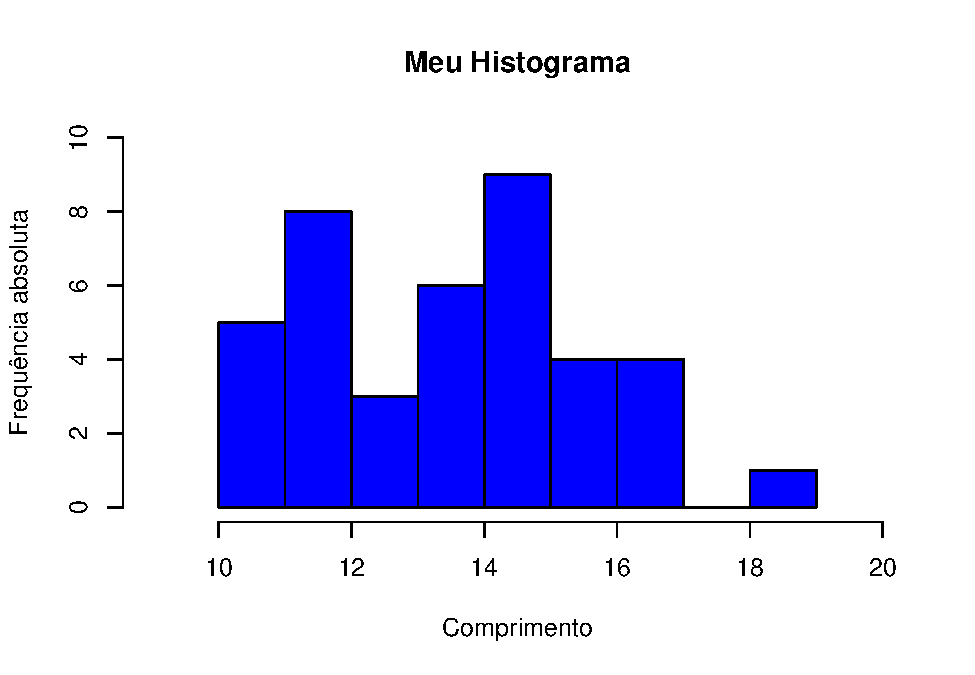
\includegraphics[width=0.7\linewidth]{livroR-1.0_files/figure-latex/comp-hist-col-1} 

}

\caption{Comprimento dos organismos da planilha dados com barras coloridas}\label{fig:comp-hist-col}
\end{figure}

Temos aqui o histograma (Figura \ref{fig:comp-hist-col}) com alguns argumentos que permitiram melhorar sua visualização. Agora é possível observar a variável comprimento e sua frequência de ocorrência.

Além disso podemos observar por meio desse que o valor mínimo observado é 10, que o máximo é 19 e que as frequências das diferentes classes de comprimento formadas variam entre 0 e aproximadamente 9. Será que isto que observamos está correto? Vamos ver no tópico a seguir (4° passo: Sumarizar os dados numericamente).

Ainda em relação ao histograma é possível ver na função \textcolor{blue}{hist()} que utilizamos diversos argumentos como: ``xlim'', ``ylim'', ``col'', ``\emph{main}'', ``xlab'' e ``ylab'', além de uma função chamada \textcolor{blue}{c()}.

\begin{itemize}
\tightlist
\item
  xlim: define os limites do eixo x;
\item
  ylim: define os limites do eixo y;
\item
  col: define as cores de preenchimento das barras;
\item
  xlab: define o nome do eixo x;
\item
  ylab: define o nome do eixo y;
\item
  \textcolor{blue}{c()}: concatena (une) valores;
\end{itemize}

\textcolor{red}{OBS: Essa função} \textcolor{blue}{c()} \textcolor{red}{é muito importante e será utilizada constantemente ao longo de seu trajeto no R.}

\hypertarget{gruxe1fico-de-barras}{%
\subsection{Gráfico de Barras}\label{gruxe1fico-de-barras}}

O gráfico de barras é um dos mais utilizados. Com ele podemos comparar valores de categorias diferentes. Por exemplo, dados onde temos números de indivíduos de diversas espécies podem ser representados em gráficos de barras, onde cada espécie será representada por uma barra.

Se já chegamos até esse ponto vamos exercitar um pouco antes de plotar o gráfico de barras. Construa a seguinte planilha no seu editor de planilhas (Figura \ref{fig:abundancia}) e nomeie-a de \textbf{abundancia}.

\begin{figure}[H]

{\centering 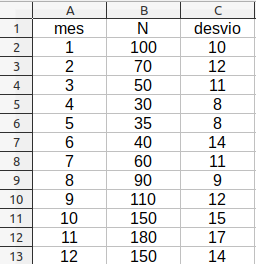
\includegraphics[width=0.4\linewidth]{/media/wilson/personaldoc/Livro_R/Série estatística passo a passo em excel e R/livroR-1.0/figures print/abundancia} 

}

\caption{Planilha de dados de abundância.}\label{fig:abundancia}
\end{figure}

Acesse a planilha abundância. Vamos inseri-la no R com o nome \textbf{abundancia}. repare que retirei o acento e as letras estão em minúsculo. Sempre que trabalharmos com linguagem de programação evite acentuações, espaços, cedilhas (ç) e atente a maiúsculas e minúsculas, pois isso pode interferir no seu código

\textcolor{red}{OBS: Se estiver iniciando o R agora lembre-se de definir o ambiente de trabalho.}

\begin{Shaded}
\begin{Highlighting}[]
\NormalTok{abundancia <-}\StringTok{ }\KeywordTok{read_excel}\NormalTok{(}\StringTok{"abundancia.xlsx"}\NormalTok{, }\DataTypeTok{col_names =} \OtherTok{TRUE}\NormalTok{)}
\end{Highlighting}
\end{Shaded}

Repare que ela está no formato *.xlsx e apresenta as seguintes variáveis: mes, N e desvio. Onde N significa o número de indivíduos observados e desvio o desvio padrão.

Vamos apenas conferir se está tudo certo com os dados usando a função \textcolor{blue}{str()}.

\begin{Shaded}
\begin{Highlighting}[]
\KeywordTok{str}\NormalTok{(abundancia)}
\end{Highlighting}
\end{Shaded}

\begin{verbatim}
## tibble[,3] [12 x 3] (S3: tbl_df/tbl/data.frame)
##  $ mes   : num [1:12] 1 2 3 4 5 6 7 8 9 10 ...
##  $ N     : num [1:12] 100 70 50 30 35 40 60 90 110 150 ...
##  $ desvio: num [1:12] 10 12 11 8 8 14 11 9 12 15 ...
\end{verbatim}

Vamos converter a variável mês em factor.

\begin{Shaded}
\begin{Highlighting}[]
\NormalTok{abundancia}\OperatorTok{$}\NormalTok{mes <-}\StringTok{ }\KeywordTok{as.factor}\NormalTok{(abundancia}\OperatorTok{$}\NormalTok{mes)}
\end{Highlighting}
\end{Shaded}

Repare que agora que sabemos os passos a realizar, da importação dos arquivos até este momento tudo ficou muito mais fácil e fluido e apenas realizamos três etapas, sendo uma delas apenas para conferir os dados.

Seguimos então para o gráfico de barras (Figura \ref{fig:bar-abu}), a fim de mostrar o número de indivíduos ao longo dos meses. Para isso utilizaremos a função \textcolor{blue}{barplot()}.

\begin{Shaded}
\begin{Highlighting}[]
\KeywordTok{barplot}\NormalTok{(abundancia}\OperatorTok{$}\NormalTok{N)}
\end{Highlighting}
\end{Shaded}

\begin{figure}[H]

{\centering 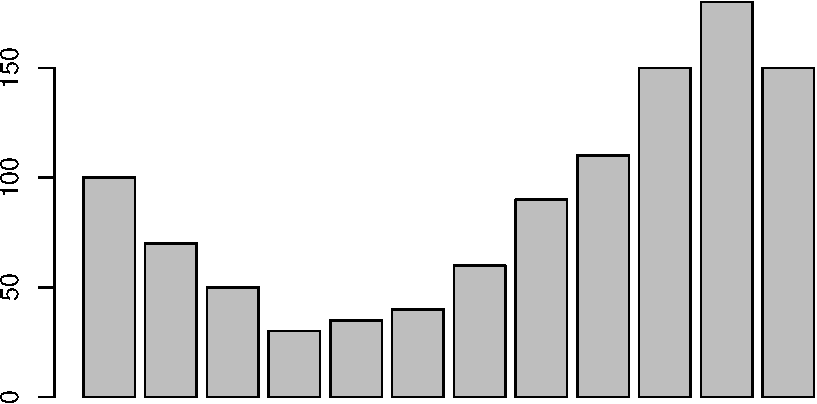
\includegraphics[width=0.7\linewidth]{livroR-1.0_files/figure-latex/bar-abu-1} 

}

\caption{Gráfico de barras com número de indivíduos da planilha abundância por mês}\label{fig:bar-abu}
\end{figure}

Assim como o histograma, o simples uso da função sem argumentos gera um gráfico de difícil análise e esteticamente não muito agradável.

Vamos portanto adicionar alguns argumentos já conhecidos e outros novos que permitirão a melhor análise do gráfico (Figura \ref{fig:bar-abu-col}).

\begin{Shaded}
\begin{Highlighting}[]
\KeywordTok{barplot}\NormalTok{(abundancia}\OperatorTok{$}\NormalTok{N,}
        \DataTypeTok{ylim =} \KeywordTok{c}\NormalTok{(}\DecValTok{0}\NormalTok{, }\DecValTok{200}\NormalTok{),}
        \DataTypeTok{xlab =} \StringTok{"Mês",}
\StringTok{        ylab = "}\NormalTok{Abundância}\StringTok{",}
\StringTok{        names.arg = abundancia$mes,}
\StringTok{        col = "}\NormalTok{green}\StringTok{")}
\end{Highlighting}
\end{Shaded}

\begin{figure}[H]

{\centering 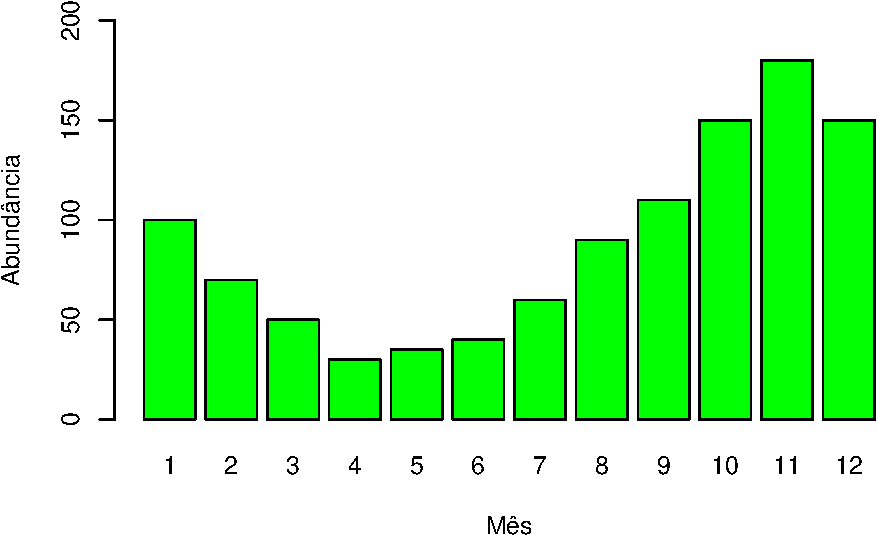
\includegraphics[width=0.7\linewidth]{livroR-1.0_files/figure-latex/bar-abu-col-1} 

}

\caption{Gráfico de barras com número de indivíduos da planilha abundância por mês, com barras coloridas}\label{fig:bar-abu-col}
\end{figure}

No código acima definimos o que será graficado, como a variável N presente no objeto abundância e informamos isso por meio do operador ``\textbf{\$}'' (cifrão). Ajustamos os limites do eixo ``y'' através do argumento ``ylim'' em 0 e 200, usando a função concatenar \textcolor{blue}{c()}. Definimos os nomes dos eixos x e y por meio dos argumentos ``xlab'' e ``ylab'', respectivamente. Definimos o nome das barras de acordo com a variável mes, também presente no objeto \textbf{abundancia} e por último definimos a cor das barras, usando o argumento ``col'', como verde.

Podemos extrair desse gráfico que a abundância dos indivíduos variam ao longo dos meses com valores menores em torno de 50 indivíduos nos meses 4, 5 e 6 e valores maiores em torno de 200 indivíduos no mês 11.

\hypertarget{gruxe1fico-de-pontos-e-de-linhas}{%
\subsection{Gráfico de Pontos e de Linhas}\label{gruxe1fico-de-pontos-e-de-linhas}}

Quando queremos representar dados quantitativos em ambos os eixos, podemos usar tanto o gráfico de pontos quanto o de linhas. Com eles geralmente podemos verificar a relação entre as variáveis (gráfico de pontos) ou a tendência dos nossos dados em ordem cronológica (gráfico de linhas). Por exemplo, podemos representar num gráfico de linhas a variação da quantidade de indivíduos de uma espécie ao longo do ano ou os valores de precipitação ao longo de décadas.

Para fazer um gráfico seja de pontos ou de linhas pelo comando básico do R (utilizamos a função \textcolor{blue}{plot()}) precisamos indicar que ambos os eixos apresentam variáveis numéricas. Portanto teremos que modificar a variável mês de fator para número. Porém não precisamos fazer isso em um comando separado podemos aplicar a função que converte uma variável em numérica dentro da função que plota o gráfico. Vamos visualizar como isso ocorre na prática (Figura \ref{fig:pon-graf}).

\begin{Shaded}
\begin{Highlighting}[]
\KeywordTok{plot}\NormalTok{(}\DataTypeTok{x =} \KeywordTok{as.numeric}\NormalTok{(abundancia}\OperatorTok{$}\NormalTok{mes), }\DataTypeTok{y =}\NormalTok{ abundancia}\OperatorTok{$}\NormalTok{N)}
\end{Highlighting}
\end{Shaded}

\begin{figure}[H]

{\centering 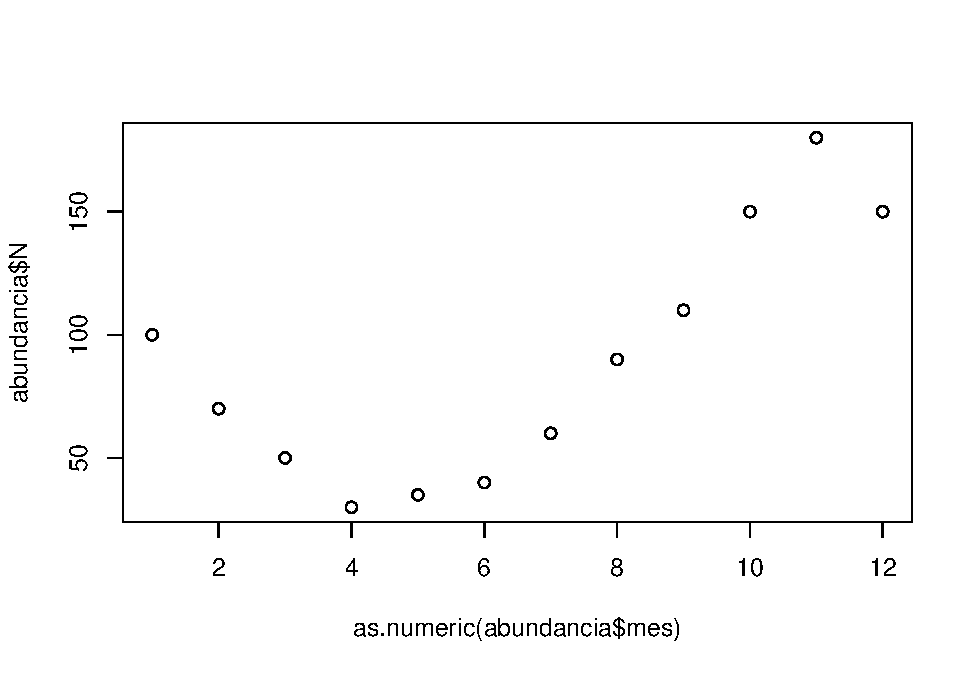
\includegraphics[width=0.7\linewidth]{livroR-1.0_files/figure-latex/pon-graf-1} 

}

\caption{Representação gráfica do número de indivíduos por mês em pontos}\label{fig:pon-graf}
\end{figure}

Pronto, na função acima aplicamos a função \textcolor{blue}{plot()} indicando os argumentos x e y que definem quem estará no eixo x e quem estará no eixo y, e para a variável que estará no eixo x (variável mês) adicionamos a função \textcolor{blue}{as.numeric()}, a qual a converte em numérico apenas para a execução do plot.

Porém a função \textcolor{blue}{plot()} não realizou um gráfico de linhas como esperado, pois para isso precisamos indica-lo por meio de argumentos. Como demonstraremos a seguir (Figura \ref{fig:lin-graf-col}).

\begin{Shaded}
\begin{Highlighting}[]
\KeywordTok{plot}\NormalTok{(}\DataTypeTok{x =} \KeywordTok{as.numeric}\NormalTok{(abundancia}\OperatorTok{$}\NormalTok{mes), }
     \DataTypeTok{y =}\NormalTok{ abundancia}\OperatorTok{$}\NormalTok{N, }
     \DataTypeTok{xlab =} \StringTok{"Mês",}
\StringTok{     ylab = "}\NormalTok{Abundância}\StringTok{",}
\StringTok{     main = "}\NormalTok{Meu gráfico de linha}\StringTok{",}
\StringTok{     ylim = c(0, 200),}
\StringTok{     type = "}\NormalTok{l}\StringTok{",}
\StringTok{     col = "}\NormalTok{green}\StringTok{",}
\StringTok{     lwd = 2)}
\end{Highlighting}
\end{Shaded}

\begin{figure}[H]

{\centering 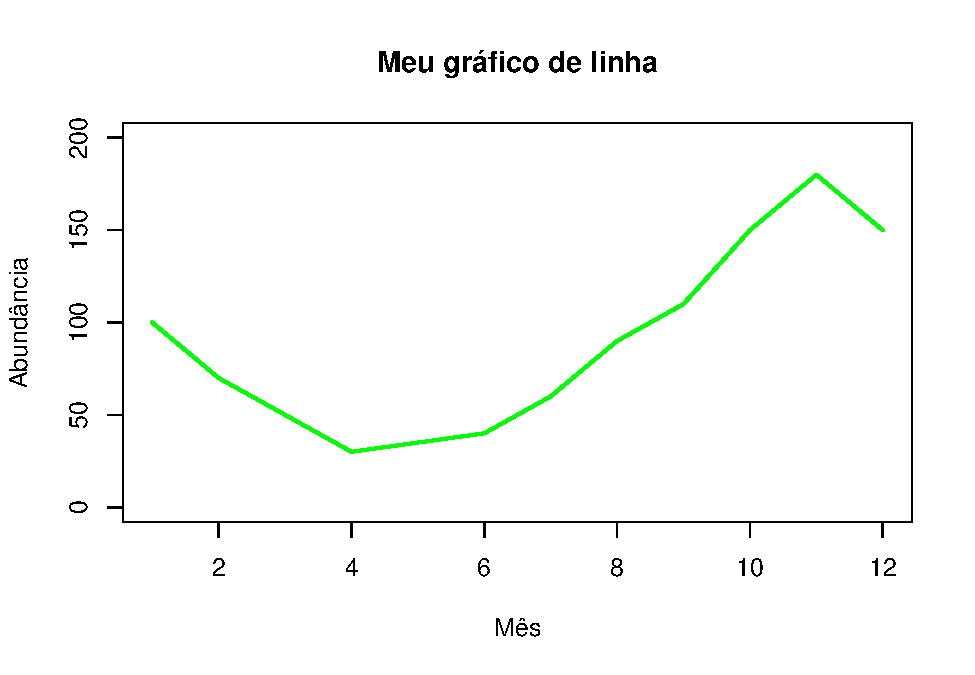
\includegraphics[width=0.7\linewidth]{livroR-1.0_files/figure-latex/lin-graf-col-1} 

}

\caption{Representação gráfica do número de indivíduos por mês em um gráfico de linhas}\label{fig:lin-graf-col}
\end{figure}

Repare que inserimos alguns argumentos novos:

\begin{itemize}
\tightlist
\item
  main: que insere o título do gráfico;
\item
  type: que define que será um gráfico de linhas;
\item
  lwd: que determina a espessura da linha;
\end{itemize}

\hypertarget{boxplot}{%
\subsection{Boxplot}\label{boxplot}}

Podemos usar os bloxplots para verificar a tendência das amostras e a distribuição destas. Quando se tem uma pequena quantidade de amostras (por exemplo, 3 réplicas) esse gráfico não é indicado. Nele também podemos verificar se temos alguma anomalia nos dados, os chamados \emph{outliers}.

Vamos voltar a nossa primeira planilha \textbf{dados} e executar um gráfico do tipo boxplot (Figura \ref{fig:box-graf}) e ver o que ele nos informa. Para isso utilizaremos a função \textcolor{blue}{boxplot()}.

\begin{Shaded}
\begin{Highlighting}[]
\KeywordTok{boxplot}\NormalTok{(}\DataTypeTok{formula =}\NormalTok{ dados}\OperatorTok{$}\NormalTok{comprimento }\OperatorTok{~}\StringTok{ }\NormalTok{dados}\OperatorTok{$}\NormalTok{ano)}
\end{Highlighting}
\end{Shaded}

\begin{figure}[H]

{\centering 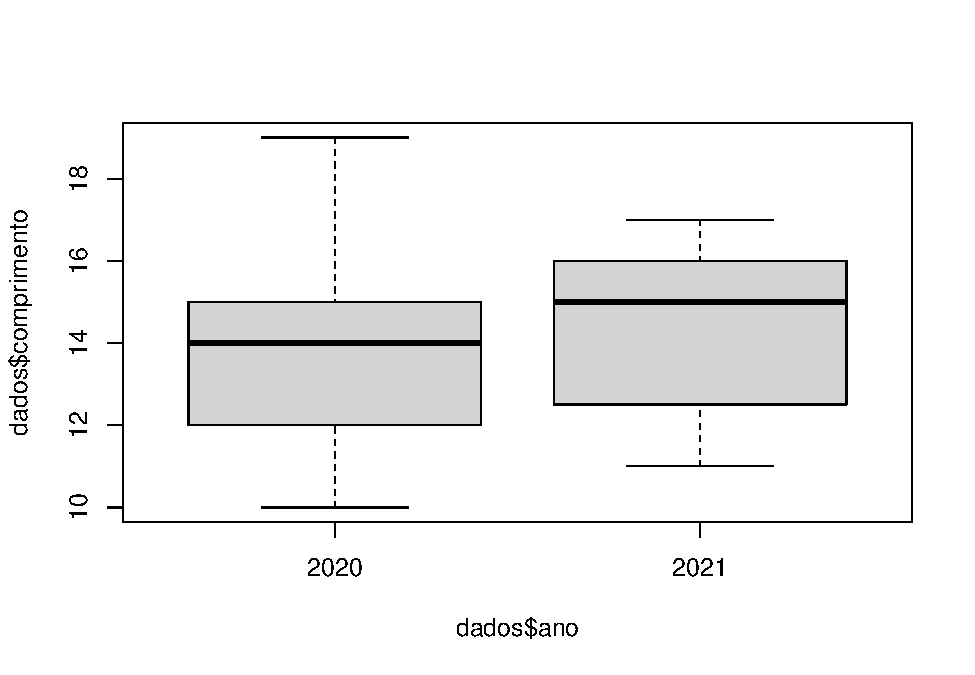
\includegraphics[width=0.7\linewidth]{livroR-1.0_files/figure-latex/box-graf-1} 

}

\caption{Gráfico tipo boxplot do comprimento por ano, da planilha dados}\label{fig:box-graf}
\end{figure}

Repare que a escrita para esse gráfico é ligeiramente diferente. Dentro desta função há um argumento chamado ``fórmula'', onde inserimos a variável independente (variável do eixo X) e a variável dependente (variável do eixo Y). Entre ambas as variáveis há o caracter ``\textasciitilde{}'' (til). A forma de ler essa escrita é a seguinte: Realize um boxplot da variável comprimento do objeto \textbf{dados} em função da variável ano do objeto \textbf{dados}. O caracter til é lido como (``em função de'')

Vamos adicionar alguns argumentos que permitem deixar o gráfico mais apresentável (Figura \ref{fig:box-graf-col}).

\begin{Shaded}
\begin{Highlighting}[]
\KeywordTok{boxplot}\NormalTok{(}\DataTypeTok{formula =}\NormalTok{ dados}\OperatorTok{$}\NormalTok{comprimento }\OperatorTok{~}\StringTok{ }\NormalTok{dados}\OperatorTok{$}\NormalTok{ano,}
        \DataTypeTok{col =} \KeywordTok{c}\NormalTok{(}\StringTok{"blue"}\NormalTok{, }\StringTok{"green"}\NormalTok{),}
        \DataTypeTok{xlab =} \StringTok{"Ano"}\NormalTok{,}
        \DataTypeTok{ylab =} \StringTok{"Comprimento"}\NormalTok{,}
        \DataTypeTok{main =} \StringTok{"Meu Boxplot"}\NormalTok{)}
\end{Highlighting}
\end{Shaded}

\begin{figure}[H]

{\centering 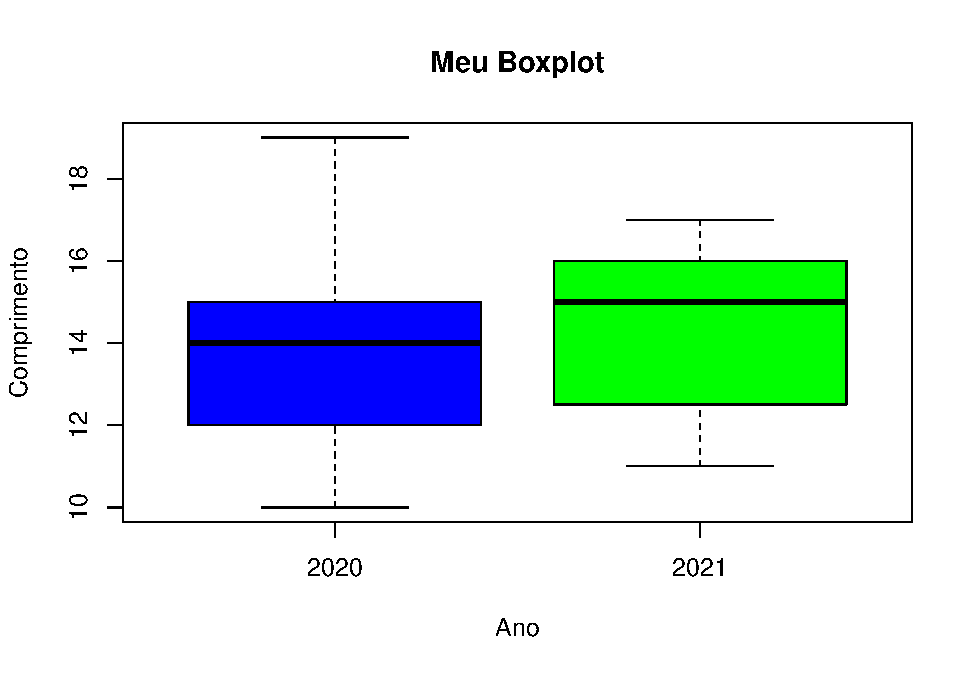
\includegraphics[width=0.7\linewidth]{livroR-1.0_files/figure-latex/box-graf-col-1} 

}

\caption{Gráfico tipo boxplot do comprimento por ano com cores por ano, da planilha dados}\label{fig:box-graf-col}
\end{figure}

Repare que não adicionamos nenhum argumento ou função diferente do que já fizemos anteriormente. Ou seja, uma vez conhecendo a função, os argumentos por vezes se repetem entre funções com o mesmo objetivo (neste caso o objetivo é gerar um gráfico).

O boxplot porém nos fornece algumas informações extras em relação ao resumo dos dados. Podemos extrair dele dados como média, mediana (segundo quartil), primeiro e terceiro quartil, assim como máximos e mínimos da variável dependente (variável do eixo y).

As linhas de cada \emph{box} (caixa) que se referem a cada um dos anos representam, em suas extremidades, os valores máximos e mínimos de comprimento de cada ano. A base e o topo de cada \emph{box} indicam o primeiro e terceiro quartil, respectivamente, do comprimento do referido ano. A linha no interior da caixa indica a mediana (segundo quartil) e a metade do \emph{box} (não marcada graficamente) indica a média.

Podemos por meio desse gráfico, então, ter uma ideia do que os dados indicam quanto as medidas de tendência central e algumas medidas de dispersão em relação as categorias presentes.

\hypertarget{passo-sumarizar-os-dados-numericamente}{%
\section{4° passo: Sumarizar os dados numericamente}\label{passo-sumarizar-os-dados-numericamente}}

Temos visto, até este ponto, como resumir os dados graficamente, de maeira geral.

Porém muitas vezes precisamos demonstrar, numericamente, quais são os valores que resumem os nosso dados. Estes valores consistem nas medidas de tendência central e nas suas medidas de dispersão.

O R permite, de maneira simples, sumarizar os dados por meio da função \textcolor{blue}{summary()}.

\begin{Shaded}
\begin{Highlighting}[]
\KeywordTok{summary}\NormalTok{(dados)}
\end{Highlighting}
\end{Shaded}

\begin{verbatim}
##    ano            local     comprimento         peso      
##  2020:20   Ambiente 1:15   Min.   :10.00   Min.   :18.00  
##  2021:20   Ambiente 2:25   1st Qu.:12.00   1st Qu.:20.00  
##                            Median :14.00   Median :21.50  
##                            Mean   :13.97   Mean   :21.73  
##                            3rd Qu.:15.00   3rd Qu.:23.00  
##                            Max.   :19.00   Max.   :28.00
\end{verbatim}

\begin{Shaded}
\begin{Highlighting}[]
\KeywordTok{summary}\NormalTok{(abundancia)}
\end{Highlighting}
\end{Shaded}

\begin{verbatim}
##       mes          N              desvio     
##  1      :1   Min.   : 30.00   Min.   : 8.00  
##  2      :1   1st Qu.: 47.50   1st Qu.: 9.75  
##  3      :1   Median : 80.00   Median :11.50  
##  4      :1   Mean   : 88.75   Mean   :11.75  
##  5      :1   3rd Qu.:120.00   3rd Qu.:14.00  
##  6      :1   Max.   :180.00   Max.   :17.00  
##  (Other):6
\end{verbatim}

Repare que ao aplicarmos esta função o R nos informou as variáveis presentes nestas planilhas e quando fator indicou quais são e quantos de cada existem. Quando númerico, nos retornou valores como média, mediana (segundo quartil), mínimo, máximo, primeiro e terceiro quartis.

As medidas de tendência central mais conhecidas e aplicadas são média, mediana e moda.

Para obtenção da média precisamos somar todos os valores e dividir pela quantidade de valores ou, no R, podemos fazer isso de maneira mais simples por meio da função \textcolor{blue}{mean()}:

\begin{Shaded}
\begin{Highlighting}[]
\KeywordTok{mean}\NormalTok{(dados}\OperatorTok{$}\NormalTok{comprimento)}
\end{Highlighting}
\end{Shaded}

\begin{verbatim}
## [1] 13.975
\end{verbatim}

Como podemos verificar a média do comprimento na planilha dados é de 13,975\footnote{Aqui estamos representando como vírgula o separador decimal. Mas o R em seu resultado utiliza o ponto (.) como separador decimal. Pois por padrão ele está configurado para o sistema númerico inglês}.

De maneira similar podemos calcular a mediana, que consiste no valor central da distribuição de valores de uma dada variável. Podemos visualiza-la por meio da função \textcolor{blue}{median()}.

\begin{Shaded}
\begin{Highlighting}[]
\KeywordTok{median}\NormalTok{(dados}\OperatorTok{$}\NormalTok{comprimento)}
\end{Highlighting}
\end{Shaded}

\begin{verbatim}
## [1] 14
\end{verbatim}

Percebe-se que o valor que se encontra no meio da distribuição da variável comprimento é 14.

Até o momento aprendemos a explorar e sumarizar nossos dados graficamente. Visualizamos também a função \textcolor{blue}{summary()} aplicada aos dados, que nos indica as medidas de tendência central média e mediana assim como outras características das variáveis como os quartis, mínimo e máximo. Essas medidas apresentadas tem como função indicar as características gerais das variáveis com as quais você está trabalhando. Porém há outras medidas que explicam os dados que são constantemente requeridas.

Medidas de dispersão indicam a propagação dos dados em torno do valor central, ou seja, são utilizadas para demonstrar a variabilidade dos dados. Quando as medidas se concentrarem em torno do centro de distribuição dos dados (baixa dispersão), quer dizer que possuem baixa variabilidade. Quando os dados apresentam uma distribuição mais ampla em torno do seu valor central (alta dispersão), significa que apresentam uma alta variabilidade.

Os limites inferior e superior de uma dada variável quantitativa são denominados mínimo e máximo e podem ser obtidos por meio das funções que calculam o mínimo e máximo. Apesar de seu resultado aparecer na função \textcolor{blue}{summary()}, que aplicamos anteriormente, podemos obtê-la separadamente para uma variável especifica. Para isso aplicamos as funções \textcolor{blue}{min()} e/ou \textcolor{blue}{max()}.

\begin{Shaded}
\begin{Highlighting}[]
\KeywordTok{min}\NormalTok{(dados}\OperatorTok{$}\NormalTok{comprimento)}
\end{Highlighting}
\end{Shaded}

\begin{verbatim}
## [1] 10
\end{verbatim}

\begin{Shaded}
\begin{Highlighting}[]
\KeywordTok{max}\NormalTok{(dados}\OperatorTok{$}\NormalTok{comprimento)}
\end{Highlighting}
\end{Shaded}

\begin{verbatim}
## [1] 19
\end{verbatim}

Uma outra forma de obter os valores máximo e mínimo é usando a função \textcolor{blue}{range()}.

\begin{Shaded}
\begin{Highlighting}[]
\KeywordTok{range}\NormalTok{(dados}\OperatorTok{$}\NormalTok{comprimento)}
\end{Highlighting}
\end{Shaded}

\begin{verbatim}
## [1] 10 19
\end{verbatim}

Novamente repare que usamos o operador cifrão (\textbf{\$}) após o nome do conjunto de dados. Como você aprendeu anteriormente ele permite acessar as variáveis que estão dentro do objeto dados.

Com os valores mínimo e máximo podemos obter nossa primeira medida de dispersão dos dados. A amplitude que consiste na diferença entre seus valores. Esta é a forma mais simples de verificar a dispersão de seus dados. A vantagem dela é fornecer a distância na qual seus dados variam mantendo-se a mesma unidade de medida.

A amplitude é utilizada para dados quantitativos, descrever a variabilidade de uma amostra, porém não para inferência estatística. Podemos calcula-la simplesmente utilizando a substração das funções que nos retornam seus valores. Veja o exemplo abaixo.

\begin{Shaded}
\begin{Highlighting}[]
\KeywordTok{max}\NormalTok{(dados}\OperatorTok{$}\NormalTok{comprimento) }\OperatorTok{-}\StringTok{ }\KeywordTok{min}\NormalTok{(dados}\OperatorTok{$}\NormalTok{comprimento)}
\end{Highlighting}
\end{Shaded}

\begin{verbatim}
## [1] 9
\end{verbatim}

Uma outra forma de realizar esta mesma operação é utilizando a função \textcolor{blue}{diff()} que calcula a diferença. Quando inserimos a função \textcolor{blue}{range()} dentro da função \textcolor{blue}{diff()} o R nos retorna o resultado da diferença dos valores obtidos pela função \textcolor{blue}{range()}. Veja o exemplo abaixo.

\begin{Shaded}
\begin{Highlighting}[]
\KeywordTok{diff}\NormalTok{(}\KeywordTok{range}\NormalTok{(dados}\OperatorTok{$}\NormalTok{comprimento))}
\end{Highlighting}
\end{Shaded}

\begin{verbatim}
## [1] 9
\end{verbatim}

O desvio padrão é uma das medidas de variação mais importantes que iremos realizar. Ele mede a distância dos valores observados em relação a sua média.

Durante a coleta de dados em estudos ambientais, o que normalmente é extraído de informação é uma fração de um todo, por exemplo, uma amostra de uma população. Portanto quando se deseja avaliar o desvio padrão, assim como outras medidas de variabilidade, devemos considerar se estamos avaliando uma amostra ou toda a população. Se uma amostra é considerada, nos referimos a ela como desvio padrão amostral e a representamos por (s) se toda a população é considerada nos referimos a ela como desvio padrão populacional e a representamos por (\(\sigma\)).

Neste livro vamos abordar e considerar o desvio padrão amostral.

Para calcular o desvio padrão utilizamos a seguinte fórmula:

\[s = \sqrt{\sum^{N}_{i = 1}\frac{(x_{i}-\overline{x})²}{N-1}}\]

Onde, \(\sum^{N}_{i=1}\) indica o somatório da expressão \(\frac{(x_{i}-\overline{x})²}{N-1}\) para \(i\) variando de 1 até o número total de elementos \(N\). \(x_{i}\) indica o valor medido da variável \(x\), \(\overline{x}\) indica a média da variável \(x\) e \(N\) indica o número total de elementos da variável \(x\).

Podemos calcular o desvio padrão a partir de suas partes, considerando sua fórmula ou a partir de uma função pré-existente no R. Vamos conferir as duas formas.

Para facilitar o entendimento do código vamos começar criando os seguintes objetos: \textbf{comp}, \textbf{com.media} e \textbf{N}.

\begin{Shaded}
\begin{Highlighting}[]
\NormalTok{comp <-}\StringTok{ }\NormalTok{dados}\OperatorTok{$}\NormalTok{comprimento}
\NormalTok{comp.media <-}\StringTok{ }\KeywordTok{mean}\NormalTok{(dados}\OperatorTok{$}\NormalTok{comprimento)}
\NormalTok{N <-}\StringTok{ }\KeywordTok{length}\NormalTok{(dados}\OperatorTok{$}\NormalTok{comprimento)}

\NormalTok{comp}
\end{Highlighting}
\end{Shaded}

\begin{verbatim}
##  [1] 10 11 15 12 17 14 19 16 15 12 14 15 12 12 14 13 12 11 14 14 13 12 11 15 12
## [26] 14 13 12 11 15 15 17 16 17 15 16 15 16 15 17
\end{verbatim}

\begin{Shaded}
\begin{Highlighting}[]
\NormalTok{comp.media}
\end{Highlighting}
\end{Shaded}

\begin{verbatim}
## [1] 13.975
\end{verbatim}

\begin{Shaded}
\begin{Highlighting}[]
\NormalTok{N}
\end{Highlighting}
\end{Shaded}

\begin{verbatim}
## [1] 40
\end{verbatim}

\begin{itemize}
\tightlist
\item
  comp: contêm os dados da variável comprimento presente na planilha dados
\item
  comp.media: contêm um dado que consiste na média da variável comprimento
\item
  N: representa a quantidade de observações presentes na variável comprimento. Repare que aqui utilizamos uma nova função chamada \textcolor{blue}{length()} a qual contabiliza o número de observações de objeto.
\end{itemize}

Agora vamos realizar o desvio padrão de 3 formass. Onde na primeira vamos entender como lemos uma função. O ideal é ler de dentro para fora. Como uma equação matemática. Mas não se assuste é mais fácil do que parece. Nas outras 2 maneiras vamos aplicar uma função pre-existente no R.

\begin{Shaded}
\begin{Highlighting}[]
\KeywordTok{sqrt}\NormalTok{((}\KeywordTok{sum}\NormalTok{((comp }\OperatorTok{-}\StringTok{ }\NormalTok{comp.media)}\OperatorTok{^}\DecValTok{2}\NormalTok{)) }\OperatorTok{/}\StringTok{ }\NormalTok{(N }\OperatorTok{-}\StringTok{ }\DecValTok{1}\NormalTok{))}
\end{Highlighting}
\end{Shaded}

\begin{verbatim}
## [1] 2.106005
\end{verbatim}

\begin{Shaded}
\begin{Highlighting}[]
\KeywordTok{sd}\NormalTok{(dados}\OperatorTok{$}\NormalTok{comprimento)}
\end{Highlighting}
\end{Shaded}

\begin{verbatim}
## [1] 2.106005
\end{verbatim}

\begin{Shaded}
\begin{Highlighting}[]
\KeywordTok{sd}\NormalTok{(comp)}
\end{Highlighting}
\end{Shaded}

\begin{verbatim}
## [1] 2.106005
\end{verbatim}

A leitura da primeira dá-se da seguinte forma:

\begin{enumerate}
\def\labelenumi{\arabic{enumi}.}
\tightlist
\item
  (comp - comp.media): Realize a diferença dos valores presentes em comp de sua média.
\item
  ((comp - comp.media)\^{}2): Eleve esses valores, obtidos da diferença, ao quadrado.
\item
  (sum((comp - comp.media)\^{}2)): Some todos os valores, obtidos pela diferença elevados ao quadrado.
\item
  (sum((comp - comp.media)\^{}2)) / (N - 1): Divide a soma dos valores da diferença elevado ao quadrado pelo número de observações menos 1.
\item
  sqrt((sum((comp - comp.media)\^{}2)) / (N - 1)): Extraia a raíz quadrada da divisão da soma dos valores da diferença elevado ao quadrado pelo número de observações menos 1.
\end{enumerate}

Repare que a leitura segue a ordem dos passos do cálculo que seria feito a mão usando a equação apresentada acima.

Mas caso não queira escrever a fórmula, o R nos fornece a função \textcolor{blue}{sd()} que pode ser aplicada a uma variável dentro de uma planilha de dados (segunda forma apresentada) ou a um vetor que contenha um conjunto de observações do seu interesse (terceira forma apresentada).

Pronto, agora entendemos como ler um código que apresenta funções dentro de funções e entendemos como realizar o desvio padrão de três formas distintas (existem diversas outras formas) no R. Agora você já pode escolher a que mais lhe agrada. Qual você prefere? Bem, essa é uma escolha sua.

Assim como o desvio padrão temos também a variância. Na variância, calculamos o grau de dispersão dos nossos dados em relação à média desses dados. Há todo um conjunto especial de análise de dados voltado para ela. Mas como poderão ver, ela não difere muito do desvio padrão, apenas pelo fato de que consiste no seu valor elevado ao quadrado, daí a variância amostral ser representada por s² enquanto que o desvio padrão é representado por s.

Partindo dessa ideia, a variância consiste em estimar o desvio padrão e eleva-lo ao quadrado (ou removermos a raíz quadrada da fórmula do desvio padrão). Vamos observar o seu resultado utilizando sua fórmula e a função predefinida pelo R.

\begin{Shaded}
\begin{Highlighting}[]
\NormalTok{(}\KeywordTok{sum}\NormalTok{((comp }\OperatorTok{-}\StringTok{ }\NormalTok{comp.media)}\OperatorTok{^}\DecValTok{2}\NormalTok{)) }\OperatorTok{/}\StringTok{ }\NormalTok{(N }\OperatorTok{-}\StringTok{ }\DecValTok{1}\NormalTok{)}
\end{Highlighting}
\end{Shaded}

\begin{verbatim}
## [1] 4.435256
\end{verbatim}

\begin{Shaded}
\begin{Highlighting}[]
\KeywordTok{sd}\NormalTok{(dados}\OperatorTok{$}\NormalTok{comprimento)}\OperatorTok{^}\DecValTok{2}
\end{Highlighting}
\end{Shaded}

\begin{verbatim}
## [1] 4.435256
\end{verbatim}

\begin{Shaded}
\begin{Highlighting}[]
\KeywordTok{var}\NormalTok{(dados}\OperatorTok{$}\NormalTok{comprimento)}
\end{Highlighting}
\end{Shaded}

\begin{verbatim}
## [1] 4.435256
\end{verbatim}

Pronto, aqui estão 3 formas de encontrar a variância de seus dados. A primeira é similar ao que realizamos anteriormente para o desvio padrão, porém sem a raíz quadrada. A segunda consiste em elevar ao quadrado o resultado do desvio padrão e a terceira é aplicando a função \textcolor{blue}{var()} à variável comprimento presente na planilha dados.

Difícil? Espero que não.

O coeficiente de variação é outra medida importante e de fácil interpretação sobre a variabilidade dos dados. Este consiste em representar a variação em torno da média em termos percentuais. Este é simples de calcular e intuitivo de interpretar.

Não há, até o momento, uma função no pacote básico do R que o calcule. Vamos calcula-lo a partir de sua fórmula matemática e ver o que ele quer dizer.

\begin{Shaded}
\begin{Highlighting}[]
\KeywordTok{sd}\NormalTok{(dados}\OperatorTok{$}\NormalTok{comprimento)}\OperatorTok{/}\KeywordTok{mean}\NormalTok{(dados}\OperatorTok{$}\NormalTok{comprimento)}\OperatorTok{*}\DecValTok{100}
\end{Highlighting}
\end{Shaded}

\begin{verbatim}
## [1] 15.0698
\end{verbatim}

Pronto, calculamos o coeficiente de variação da variável comprimento e obtivemos uma variação em torno da média de ±15,07\%.

Com isso verificamos as principais medidas de tendência central e dispersão. Mas fica, aqui, uma questão. Como incorpora-las aos gráficos para que assim possamos resumir os dados graficamente de maneira mais completa?

Vamos utilizar nossa planilha dados e verificar a média do comprimento e do peso por ano e por ambiente e incorporar em cada um dos gráficos seus respectivos desvios padrões.

Neste caso vamos primeiro precisar organizar os dados que queremos plotar. Como desejamos plotar a média do comprimento por ano e ambiente com seus respectivos desvios padrões, vamos primeiro construir passo a passo uma tabela que apresente 4 colunas. A primeira com o ano, a segunda com ambiente, a terceira com a média do comprimento e a última com o desvio padrão.

Para isso vamos utilizar a função \textcolor{blue}{split()}, que fragmenta um \emph{data frame} em função de algum fator. Neste primeiro momento, vamos fragmentar o objeto \textbf{dados} em função do ano e alocar esses dois novos conjuntos de dados em um novo objeto chamado \textbf{dados.2}. Posteriormente vamos criar um objeto chamado \textbf{ano.2020} onde vamos alocar o primeiro objeto (referente ao ano de 2020) que está dentro de \textbf{dados.2} e um segundo objeto chamado \textbf{ano.2021} onde vamos alocar o segundo objeto (referente ao ano de 2021) que está dentro de \textbf{dados.2}. Veja os comandos abaixo.

\begin{Shaded}
\begin{Highlighting}[]
\NormalTok{dados}\FloatTok{.2}\NormalTok{ <-}\StringTok{ }\KeywordTok{split}\NormalTok{(}\DataTypeTok{x =}\NormalTok{ dados, }\DataTypeTok{f =}\NormalTok{ dados}\OperatorTok{$}\NormalTok{ano)}
\NormalTok{ano}\FloatTok{.2020}\NormalTok{ <-}\StringTok{ }\NormalTok{dados}\FloatTok{.2}\OperatorTok{$}\StringTok{`}\DataTypeTok{2020}\StringTok{`}
\NormalTok{ano}\FloatTok{.2021}\NormalTok{ <-}\StringTok{ }\NormalTok{dados}\FloatTok{.2}\OperatorTok{$}\StringTok{`}\DataTypeTok{2021}\StringTok{`}
\end{Highlighting}
\end{Shaded}

Repare que foram criados no environment três novos objetos: \textbf{dados.2} o qual consiste em um objeto da classe lista que contêm o objeto \textbf{dados} separado por ano; \textbf{ano.2020} que consiste no objeto da classe \emph{data frame} (mesma classe do objeto \textbf{dados}) que contêm as informações referentes, somente ao ano de 2020; e o objeto \textbf{ano.2021}, similar ao anterior, porém com as informações referentes ao ano de 2021.

A seguir vamos aplicar o mesmo racíocinio lógico para fragmentar os objetos \textbf{ano.2020} e \textbf{ano.2021} por locais.

\begin{Shaded}
\begin{Highlighting}[]
\NormalTok{ano.}\FloatTok{2020.}\NormalTok{local <-}\StringTok{ }\KeywordTok{split}\NormalTok{(}\DataTypeTok{x =}\NormalTok{ ano}\FloatTok{.2020}\NormalTok{, }\DataTypeTok{f =}\NormalTok{ ano}\FloatTok{.2020}\OperatorTok{$}\NormalTok{local)}
\NormalTok{ano.}\FloatTok{2021.}\NormalTok{local <-}\StringTok{ }\KeywordTok{split}\NormalTok{(}\DataTypeTok{x =}\NormalTok{ ano}\FloatTok{.2021}\NormalTok{, }\DataTypeTok{f =}\NormalTok{ ano}\FloatTok{.2021}\OperatorTok{$}\NormalTok{local)}
\NormalTok{ano.}\FloatTok{2020.}\NormalTok{local}\FloatTok{.1}\NormalTok{ <-}\StringTok{ }\NormalTok{ano.}\FloatTok{2020.}\NormalTok{local}\OperatorTok{$}\StringTok{`}\DataTypeTok{Ambiente 1}\StringTok{`}
\NormalTok{ano.}\FloatTok{2020.}\NormalTok{local}\FloatTok{.2}\NormalTok{ <-}\StringTok{ }\NormalTok{ano.}\FloatTok{2020.}\NormalTok{local}\OperatorTok{$}\StringTok{`}\DataTypeTok{Ambiente 2}\StringTok{`}
\NormalTok{ano.}\FloatTok{2021.}\NormalTok{local}\FloatTok{.1}\NormalTok{ <-}\StringTok{ }\NormalTok{ano.}\FloatTok{2021.}\NormalTok{local}\OperatorTok{$}\StringTok{`}\DataTypeTok{Ambiente 1}\StringTok{`}
\NormalTok{ano.}\FloatTok{2021.}\NormalTok{local}\FloatTok{.2}\NormalTok{ <-}\StringTok{ }\NormalTok{ano.}\FloatTok{2021.}\NormalTok{local}\OperatorTok{$}\StringTok{`}\DataTypeTok{Ambiente 2}\StringTok{`}
\end{Highlighting}
\end{Shaded}

Pronto! Dividimos nossos dados de acordo com os fatores que desejamos (ano e local) utilizando o argumento ``f'' da função \textcolor{blue}{split()}. Agora vamos obter as métricas média e desvio padrão para cada ano de cada local. Para isso vamos criar novos objetos que alocam esses dados.

\begin{Shaded}
\begin{Highlighting}[]
\NormalTok{ano.}\FloatTok{2020.}\NormalTok{local.}\FloatTok{1.}\NormalTok{comp.media <-}\StringTok{ }\KeywordTok{mean}\NormalTok{(ano.}\FloatTok{2020.}\NormalTok{local}\FloatTok{.1}\OperatorTok{$}\NormalTok{comprimento)}
\NormalTok{ano.}\FloatTok{2020.}\NormalTok{local.}\FloatTok{1.}\NormalTok{comp.dp <-}\StringTok{ }\KeywordTok{sd}\NormalTok{(ano.}\FloatTok{2020.}\NormalTok{local}\FloatTok{.1}\OperatorTok{$}\NormalTok{comprimento)}
\NormalTok{ano.}\FloatTok{2020.}\NormalTok{local.}\FloatTok{2.}\NormalTok{comp.media <-}\StringTok{ }\KeywordTok{mean}\NormalTok{(ano.}\FloatTok{2020.}\NormalTok{local}\FloatTok{.2}\OperatorTok{$}\NormalTok{comprimento)}
\NormalTok{ano.}\FloatTok{2020.}\NormalTok{local.}\FloatTok{2.}\NormalTok{comp.dp <-}\StringTok{ }\KeywordTok{sd}\NormalTok{(ano.}\FloatTok{2020.}\NormalTok{local}\FloatTok{.2}\OperatorTok{$}\NormalTok{comprimento)}
\NormalTok{ano.}\FloatTok{2021.}\NormalTok{local.}\FloatTok{1.}\NormalTok{comp.media <-}\StringTok{ }\KeywordTok{mean}\NormalTok{(ano.}\FloatTok{2021.}\NormalTok{local}\FloatTok{.1}\OperatorTok{$}\NormalTok{comprimento)}
\NormalTok{ano.}\FloatTok{2021.}\NormalTok{local.}\FloatTok{1.}\NormalTok{comp.dp <-}\StringTok{ }\KeywordTok{sd}\NormalTok{(ano.}\FloatTok{2021.}\NormalTok{local}\FloatTok{.1}\OperatorTok{$}\NormalTok{comprimento)}
\NormalTok{ano.}\FloatTok{2021.}\NormalTok{local.}\FloatTok{2.}\NormalTok{comp.media <-}\StringTok{ }\KeywordTok{mean}\NormalTok{(ano.}\FloatTok{2021.}\NormalTok{local}\FloatTok{.2}\OperatorTok{$}\NormalTok{comprimento)}
\NormalTok{ano.}\FloatTok{2021.}\NormalTok{local.}\FloatTok{2.}\NormalTok{comp.dp <-}\StringTok{ }\KeywordTok{sd}\NormalTok{(ano.}\FloatTok{2021.}\NormalTok{local}\FloatTok{.2}\OperatorTok{$}\NormalTok{comprimento)}
\end{Highlighting}
\end{Shaded}

Pronto! Média e desvio padrão do comprimento calculado para cada ano e local e alocados em seus respectivos objetos. Agora vamos unir esses resultados, por meio da função \textcolor{blue}{c()} em um objeto com os dados referentes a média \textbf{dados.media} e um outro com o desvio padrão \textbf{dados.dp}.

\begin{Shaded}
\begin{Highlighting}[]
\NormalTok{dados.media <-}\StringTok{ }\KeywordTok{c}\NormalTok{(ano.}\FloatTok{2020.}\NormalTok{local.}\FloatTok{1.}\NormalTok{comp.media,}
\NormalTok{                 ano.}\FloatTok{2020.}\NormalTok{local.}\FloatTok{2.}\NormalTok{comp.media,}
\NormalTok{                 ano.}\FloatTok{2021.}\NormalTok{local.}\FloatTok{1.}\NormalTok{comp.media,}
\NormalTok{                 ano.}\FloatTok{2021.}\NormalTok{local.}\FloatTok{2.}\NormalTok{comp.media)}
\NormalTok{dados.dp <-}\StringTok{ }\KeywordTok{c}\NormalTok{(ano.}\FloatTok{2020.}\NormalTok{local.}\FloatTok{1.}\NormalTok{comp.dp,}
\NormalTok{              ano.}\FloatTok{2020.}\NormalTok{local.}\FloatTok{2.}\NormalTok{comp.dp,}
\NormalTok{              ano.}\FloatTok{2021.}\NormalTok{local.}\FloatTok{1.}\NormalTok{comp.dp,}
\NormalTok{              ano.}\FloatTok{2021.}\NormalTok{local.}\FloatTok{2.}\NormalTok{comp.dp)}
\end{Highlighting}
\end{Shaded}

Agora, vamos criar as variáveis categóricas ano e local para adicionar aos dados de médias e desvios e unir esses objetos em um \emph{data frame} chamado \textbf{dados.3}. Posteriormente vamos conferir as classes das variáveis.

Para isso durante este processo utilizaremos duas funções que não haviamos utilizado antes. As funções \textcolor{blue}{as.data.frame()} que faz com que um conjunto de objetos sejam convertidos em \emph{data frame} e \textcolor{blue}{cbind()} o qual une objetos como colunas. Essas funções também serão comumente utilizadas durante seus passos iniciais no R.

\begin{Shaded}
\begin{Highlighting}[]
\NormalTok{ano <-}\StringTok{ }\KeywordTok{c}\NormalTok{(}\StringTok{"2020"}\NormalTok{, }\StringTok{"2020"}\NormalTok{, }\StringTok{"2021"}\NormalTok{, }\StringTok{"2021"}\NormalTok{)}
\NormalTok{local <-}\StringTok{ }\KeywordTok{c}\NormalTok{(}\StringTok{"Ambiente 1"}\NormalTok{, }\StringTok{"Ambiente 2"}\NormalTok{, }\StringTok{"Ambiente 1"}\NormalTok{, }\StringTok{"Ambiente 2"}\NormalTok{)}
\NormalTok{dados}\FloatTok{.3}\NormalTok{ <-}\StringTok{ }\KeywordTok{as.data.frame}\NormalTok{(}\KeywordTok{cbind}\NormalTok{(ano, local, dados.media, dados.dp))}
\KeywordTok{str}\NormalTok{(dados}\FloatTok{.3}\NormalTok{)}
\end{Highlighting}
\end{Shaded}

\begin{verbatim}
## 'data.frame':    4 obs. of  4 variables:
##  $ ano        : chr  "2020" "2020" "2021" "2021"
##  $ local      : chr  "Ambiente 1" "Ambiente 2" "Ambiente 1" "Ambiente 2"
##  $ dados.media: chr  "14.1" "13.1" "13" "14.8"
##  $ dados.dp   : chr  "2.84604989415154" "1.28668393770792" "1.58113883008419" "1.93464651625488"
\end{verbatim}

\begin{Shaded}
\begin{Highlighting}[]
\NormalTok{dados}\FloatTok{.3}\OperatorTok{$}\NormalTok{ano <-}\StringTok{ }\KeywordTok{as.factor}\NormalTok{(dados}\FloatTok{.3}\OperatorTok{$}\NormalTok{ano)}
\NormalTok{dados}\FloatTok{.3}\OperatorTok{$}\NormalTok{local <-}\StringTok{ }\KeywordTok{as.factor}\NormalTok{(dados}\FloatTok{.3}\OperatorTok{$}\NormalTok{local)}
\NormalTok{dados}\FloatTok{.3}\OperatorTok{$}\NormalTok{dados.media <-}\StringTok{ }\KeywordTok{as.numeric}\NormalTok{(dados}\FloatTok{.3}\OperatorTok{$}\NormalTok{dados.media)}
\NormalTok{dados}\FloatTok{.3}\OperatorTok{$}\NormalTok{dados.dp <-}\StringTok{ }\KeywordTok{as.numeric}\NormalTok{(dados}\FloatTok{.3}\OperatorTok{$}\NormalTok{dados.dp)}
\end{Highlighting}
\end{Shaded}

Vejamos nosso resultado final executando o nome do nosso objeto \textbf{dados.3}.

\begin{Shaded}
\begin{Highlighting}[]
\NormalTok{dados}\FloatTok{.3}
\end{Highlighting}
\end{Shaded}

\begin{verbatim}
##    ano      local dados.media dados.dp
## 1 2020 Ambiente 1        14.1 2.846050
## 2 2020 Ambiente 2        13.1 1.286684
## 3 2021 Ambiente 1        13.0 1.581139
## 4 2021 Ambiente 2        14.8 1.934647
\end{verbatim}

Pronto! depois de alguns (muitos) passos conseguimos construir nossa nova tabela com os dados resumidos.

É um processo longo porém necessário para se acostumar com o ambiente de trabalho e a linguagem R. Há caminhos mais rápidos e tão eficientes quanto. Que se tornam úteis quando lidamos com muitas categorias dentro de uma variável. Contudo para isso é necessário a instalação de algum pacote (Há vários pacotes que apresentam funções que permitem a realização deste processo de maneira mais rápida e eficiente). Vamos utilizar um exemplo começando pela instalação do pacote chamado \textcolor{brown}{Rmisc}.

O comando abaixo realiza a instalação desse pacote. Conforme já fizemos com o pacote \textcolor{brown}{readxl}.

\begin{Shaded}
\begin{Highlighting}[]
\KeywordTok{install.packages}\NormalTok{(}\StringTok{"Rmisc"}\NormalTok{)}
\end{Highlighting}
\end{Shaded}

Após instalado vamos carrega-lo pelo comando a seguir. Conforme já fizemos com o pacote \textcolor{brown}{readxl}.

\begin{Shaded}
\begin{Highlighting}[]
\KeywordTok{library}\NormalTok{(Rmisc)}
\end{Highlighting}
\end{Shaded}

Agora vamos conhecer a função \textcolor{blue}{summarySE()} deste pacote o qual realiza os passos que fizemos anteriormente e ainda apresenta outros resultados. Mas iremos focar na média e desvio padrão.

\begin{Shaded}
\begin{Highlighting}[]
\NormalTok{resultado <-}\StringTok{ }\KeywordTok{summarySE}\NormalTok{(}\DataTypeTok{data =}\NormalTok{ dados, }
                       \DataTypeTok{measurevar =} \StringTok{"comprimento"}\NormalTok{, }
                       \DataTypeTok{groupvars =} \KeywordTok{c}\NormalTok{(}\StringTok{"ano"}\NormalTok{, }\StringTok{"local"}\NormalTok{))}
\NormalTok{resultado}
\end{Highlighting}
\end{Shaded}

\begin{verbatim}
##    ano      local  N comprimento       sd        se        ci
## 1 2020 Ambiente 1 10        14.1 2.846050 0.9000000 2.0359414
## 2 2020 Ambiente 2 10        13.1 1.286684 0.4068852 0.9204382
## 3 2021 Ambiente 1  5        13.0 1.581139 0.7071068 1.9632432
## 4 2021 Ambiente 2 15        14.8 1.934647 0.4995236 1.0713715
\end{verbatim}

Repare que a função \textcolor{blue}{summarySE()} apresenta, basicamente, 3 argumentos, ``data'' que pede que se insira a planilha a ser utilizada, ``measurevar'' o qual pede a variável quantitativa que será sumarizada e ``groupvars'' o qual pede as variáveis categóricas\footnote{Repare que usamos a função concatenar \textcolor{blue}{c()} para agrupar as 2 variáveis categóricas de interesse.} segundo as quais a variável mensurável será agrupada. Observe também que para esta função as variáveis devem ser colocadas entre aspas.

Pronto! Com a função \textcolor{blue}{summarySE()} realizamos os mesmos passos que antes e guardamos o resultado dentro de um objeto chamado \textbf{resultado}. Repare que essa função nos resumiu os dados de comprimento de acordo com as duas variáveis categóricas que indicamos: ano e local. Em seu resumo ele nos forneceu, na seguinte ordem, as colunas: ano, local, N (número de observações), comprimento (média do comprimento), sd (desvio padrão), se (erro padrão) e ci (intervalo de confiança de 95\%).

\textcolor{red}{OBS: Este é um exemplo sobre a vantagem e importância de usar funções que estão presentes em outros pacotes.}

Agora vamos usar o objeto \textbf{resultado} para desenvolver o gráfico de barras com o erro padrão (Figura \ref{fig:bar-ep}). Porém para este caso, teremos que guardar nosso gráfico dentro de algum objeto, neste caso chamamos o objeto de \textbf{grafico}. Após o gráfico ser criado devemos utilizar a função \textcolor{blue}{arrows()} que nos permite adicionar as barras de desvio padrão no nosso gráfico.

\begin{Shaded}
\begin{Highlighting}[]
\NormalTok{grafico <-}\StringTok{ }\KeywordTok{barplot}\NormalTok{(}\DataTypeTok{formula =}\NormalTok{ comprimento }\OperatorTok{~}\StringTok{ }\NormalTok{ano }\OperatorTok{+}\StringTok{ }\NormalTok{local,}
                   \DataTypeTok{data =}\NormalTok{ resultado,}
                   \DataTypeTok{beside =} \OtherTok{TRUE}\NormalTok{,}
                   \DataTypeTok{col =} \KeywordTok{c}\NormalTok{(}\StringTok{"red"}\NormalTok{, }\StringTok{"blue"}\NormalTok{),}
                   \DataTypeTok{ylim =} \KeywordTok{c}\NormalTok{(}\DecValTok{0}\NormalTok{, }\DecValTok{30}\NormalTok{),}
                   \DataTypeTok{ylab =} \StringTok{"Comprimento médio (cm)"}\NormalTok{,}
                   \DataTypeTok{legend.text =} \OtherTok{TRUE}\NormalTok{)}
\KeywordTok{arrows}\NormalTok{(}\DataTypeTok{x0 =}\NormalTok{ grafico,}
       \DataTypeTok{y0 =}\NormalTok{ resultado}\OperatorTok{$}\NormalTok{comprimento }\OperatorTok{+}\StringTok{ }\NormalTok{resultado}\OperatorTok{$}\NormalTok{sd,}
       \DataTypeTok{y1 =}\NormalTok{ resultado}\OperatorTok{$}\NormalTok{comprimento }\OperatorTok{-}\StringTok{ }\NormalTok{resultado}\OperatorTok{$}\NormalTok{sd,}
       \DataTypeTok{code =} \DecValTok{3}\NormalTok{,}
       \DataTypeTok{angle =} \DecValTok{90}\NormalTok{,}
       \DataTypeTok{length =} \FloatTok{0.05}\NormalTok{)}
\end{Highlighting}
\end{Shaded}

\begin{figure}[H]

{\centering 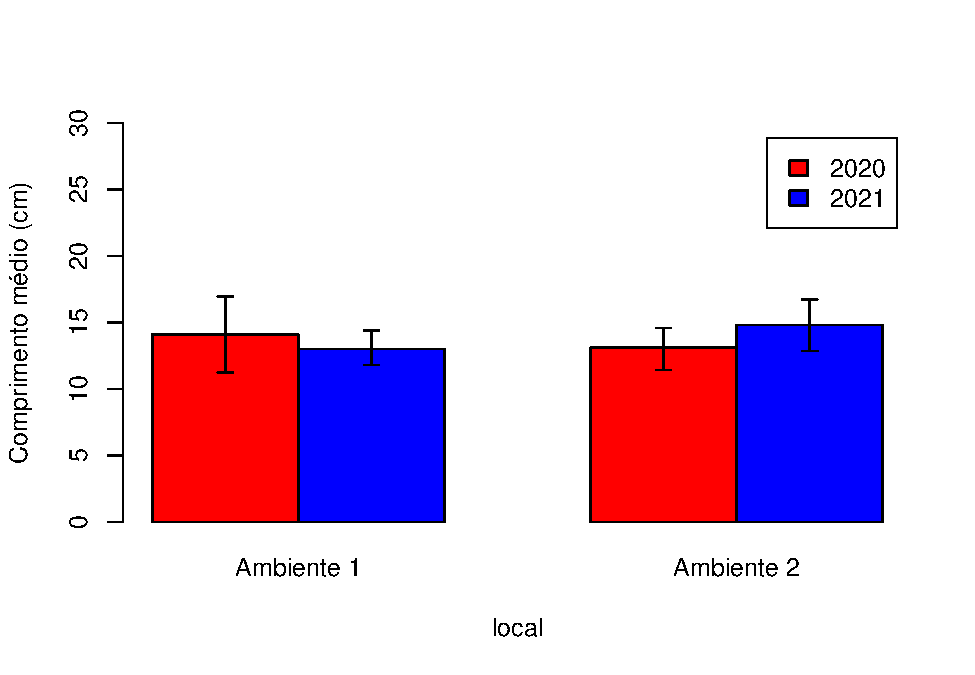
\includegraphics[width=0.7\linewidth]{livroR-1.0_files/figure-latex/bar-ep-1} 

}

\caption{Gráfico de barras com erro padrão do comprimento por ano e local, da planilha resultado (derivada da planilha dados)}\label{fig:bar-ep}
\end{figure}

Note que na função \textcolor{blue}{barplot()} utilizamos algumas mudanças em relação ao que fizemos anteriormente, como os argumentos ``formula''\footnote{similar a função \textcolor{blue}{boxplot}.} o qual indica a variável resposta em função das variáveis categóricas o qual será plotado (caso altere a ordem ano + local para local + ano a ordem do gráfico também será alterado. Teste você mesmo, veja o acontece). Neste caso, como temos mais de uma variável categórica adicionamos um argumento novo chamado ``legend.text'' o qual adiciona uma legenda ao gráfico.

A função \textcolor{blue}{arrows()} que adicionou as barras de desvios no gráfico apresenta alguns argumentos diferentes do que já vimos em outros gráficos.

\begin{itemize}
\tightlist
\item
  x0: o qual indica o objeto onde o gráfico foi armazenado;
\item
  y0: o qual é escrito como uma operação matemática onde devemos incluir o valor da média + coluna onde está a variável referente ao desvio;
\item
  y1: o qual é escrito como uma operação matemática onde devemos incluir o valor da média - coluna onde está a variável referente ao desvio;
\item
  code: determina o tipo de seta que será plotada;
\item
  angle: é o ângulo da haste da barra até a ponta;
\item
  length: é o comprimento das bordas da barra;
\end{itemize}

Terminamos de construir e entender os componentes do nosso primeiro gráfico com suas barras de erro.

O principal para construção desse gráfico consiste em entender como organizar os dados a serem graficados. Ao se usar a função \textcolor{blue}{barplot()} para construção do gráfico de barras com os desvios, devemos ter uma ou mais colunas com as categorias, outra com os valores que desejamos e outra com os valores dos desvios.

Vamos realizar um segundo tipo de gráfico onde temos apenas uma variável categórica e seus respectivos desvios. Para isso utilizaremos nosso conjunto de dados abundancia (lembre-se que mes é uma variável categórica e deve ser identificada como fator) (Figura \ref{fig:bar-ep-abu}).

Neste conjunto de dados não precisamos reorganiza-los pois já se encontram organizados e já temos os valores dos desvios.

\begin{Shaded}
\begin{Highlighting}[]
\NormalTok{grafico <-}\StringTok{ }\KeywordTok{barplot}\NormalTok{(abundancia}\OperatorTok{$}\NormalTok{N,}
                   \DataTypeTok{ylim =} \KeywordTok{c}\NormalTok{(}\DecValTok{0}\NormalTok{, }\DecValTok{200}\NormalTok{),}
                   \DataTypeTok{xlab =} \StringTok{"Mês",}
\StringTok{                   ylab = "}\NormalTok{Abundância}\StringTok{",}
\StringTok{                   names.arg = abundancia$mes,}
\StringTok{                   col = "}\NormalTok{green}\StringTok{")}
\StringTok{arrows(x0 = grafico,}
\StringTok{       y0 = abundancia$N + abundancia$desvio,}
\StringTok{       y1 = abundancia$N - abundancia$desvio,}
\StringTok{       code = 3,}
\StringTok{       angle = 90,}
\StringTok{       length = 0.05)}
\end{Highlighting}
\end{Shaded}

\begin{figure}[H]

{\centering 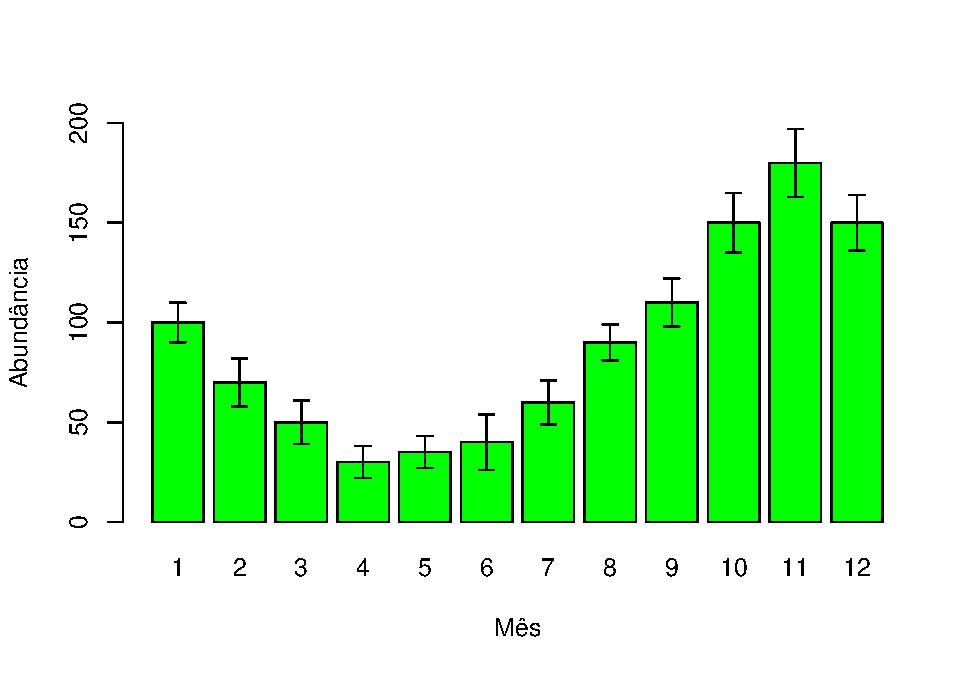
\includegraphics[width=0.7\linewidth]{livroR-1.0_files/figure-latex/bar-ep-abu-1} 

}

\caption{Gráfico de barras com erro padrão da abundância por mês da planilha abundância}\label{fig:bar-ep-abu}
\end{figure}

Repare que é a mesma coisa que fizemos anteriormente,porém com outro conjunto de dados.

\hypertarget{considerauxe7uxf5es}{%
\section{Considerações}\label{considerauxe7uxf5es}}

Ao longo dos tópicos abordados neste capítulo demonstramos as etapas mais importantes e de diversos modos para nossa trajetória inicial e necessária no R, desde a definição do ambiente de trabalho, passando pela importação da planilha de dados, verificação e ajuste dos dados e sua sumarização gráfica e numérica (Figura \ref{fig:resumo1}).

Durante nosso percurso neste livro realizaremos mais gráficos aliados as análises estatísticas básicas comumente utilizadas. Não se assuste com a quantidade de etapas, funções, argumentos e nomes, eles irão se repetir tantas e tantas vezes daqui em diante que você não esquecerá. O aprendizado do R é exponencial e ele lhe permitirá entender como nunca o universo da análise de dados adequando-o para seu campo de atuação.

\begin{figure}[H]

{\centering 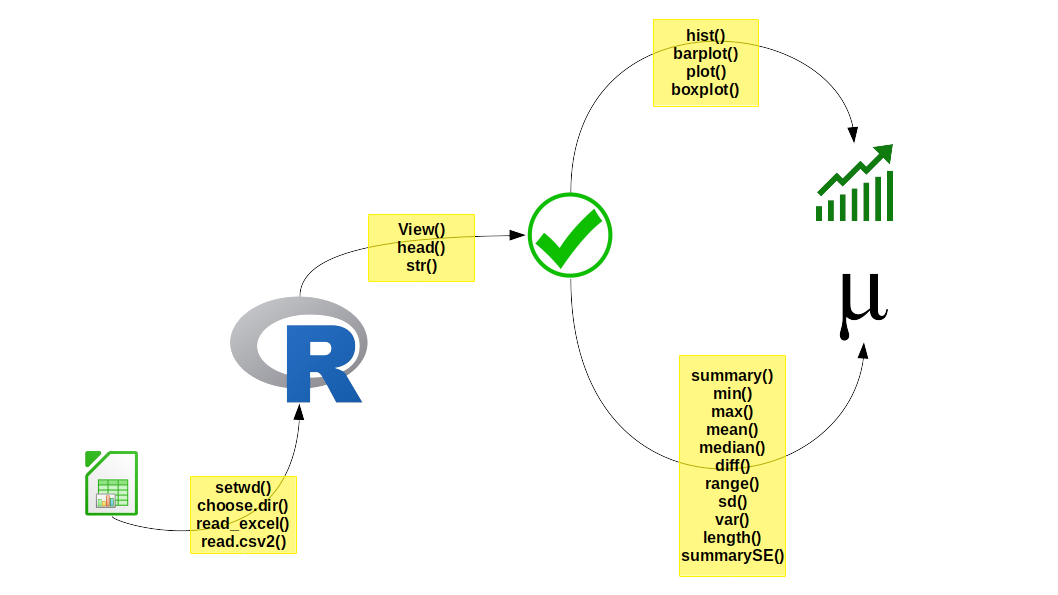
\includegraphics[width=1\linewidth]{/media/wilson/personaldoc/Livro_R/Série estatística passo a passo em excel e R/livroR-1.0/figures print/resumo1} 

}

\caption{Resumo dos passos abordados no capítulo: da definição do ambiente de trabalho até a sumarização dos dados.}\label{fig:resumo1}
\end{figure}

\hypertarget{exercuxedcios-1}{%
\section{Exercícios}\label{exercuxedcios-1}}

\begin{enumerate}
\def\labelenumi{\arabic{enumi})}
\tightlist
\item
  Para iniciarmos nosso trabalho no R precisamos saber importar os dados com os quais iremos trabalhar. Porém alguns passos são fundamentais antes da importação. Qual das opções a seguir contêm as funções, em ordem, que contemplam esses passos.
\end{enumerate}

\begin{enumerate}
\def\labelenumi{(\alph{enumi})}
\tightlist
\item
  setwd(); choose.dir(); as.factor() e readxl()
\item
  setwd(); choose.dir(); readxl()
\item
  library(); setwd(); choose.dir()
\item
  choose.dir(); setwd(); library()
\item
  choose.dir(); setwd()
\end{enumerate}

\begin{enumerate}
\def\labelenumi{\arabic{enumi})}
\setcounter{enumi}{1}
\tightlist
\item
  Ao importarmos nossos dados é importante saber a extensão em que os arquivos são encontrados (ex: *.csv ou *.xlsx). A função para importação dos dados é determinada pela extensão dos arquivos em que os dados se encontram. Qual as opções abaixo melhor apresenta os comandos responsáveis por importar um arquivo em *.csv e outro em *.xlsx?
\end{enumerate}

\begin{enumerate}
\def\labelenumi{(\alph{enumi})}
\tightlist
\item
  read\_csv(file = ``dados.csv'', header = TRUE, sep = ``,''); read.excel(path = ``dados.xlsx'', col\_names = TRUE)
\item
  read\_csv(file = ``planilha.csv'', header = TRUE, sep = ``;''); read\_excel(path = ``planilha.xlsx'', col\_names = TRUE)
\item
  read.csv(path = ``planilha.csv'', header = TRUE, sep = ``,''); read\_excel(file = ``planilha.xlsx'', col\_names = TRUE)
\item
  read.csv(file = ``dados.csv'', header = TRUE, sep = ``;''); read\_excel(path = ``planilha.xlsx'', col\_names = TRUE)
\item
  read.csv(file = ``planilha.csv'', header = TRUE, sep = ``,''); read.excel(path = ``planilha.xlsx'', col\_names = TRUE)
\end{enumerate}

\begin{enumerate}
\def\labelenumi{\arabic{enumi})}
\setcounter{enumi}{2}
\tightlist
\item
  Durante o processo de importação dos dados é necessário checar se todas as variáveis foram entendidas pelo R como elas devem ser (ex. se determinada variável foi identificada como fator ao invés de numérico ou caracter). Para isso algumas funções são importantes para checar e alterar se necessário. Qual das opções abaixo indica as funções que permitem checar e alterar as variáveis, se necessário.
\end{enumerate}

\begin{enumerate}
\def\labelenumi{(\alph{enumi})}
\tightlist
\item
  checar: View(), summary(); alterar: as.factor(), as.numeric(), as.data.frame()
\item
  checar: View(), str(); alterar: as.factor(), as.numeric(), as.integer()
\item
  checar: str(), as.data.frame(); alterar: as.data.frame(), as.numeric(), as.caracter()
\item
  checar: str(), summary(); alterar: as.caracter(), as.factor(), as.numeric()
\item
  checar: View(), as.data.frame(); alterar: as.integer(), as.numeric(), as.factor()
\end{enumerate}

\begin{enumerate}
\def\labelenumi{\arabic{enumi})}
\setcounter{enumi}{3}
\tightlist
\item
  O R apresenta em alguns de seus pacotes conjuntos de dados que nos permitem fazer análises. Usando o conjunto de dados chamado \textbf{iris}, o qual pode ser carregado usando a função \textcolor{blue}{data()}. Qual das opções abaixo apresenta o comando para gerar o gráfico apresentado?
\end{enumerate}

\begin{center}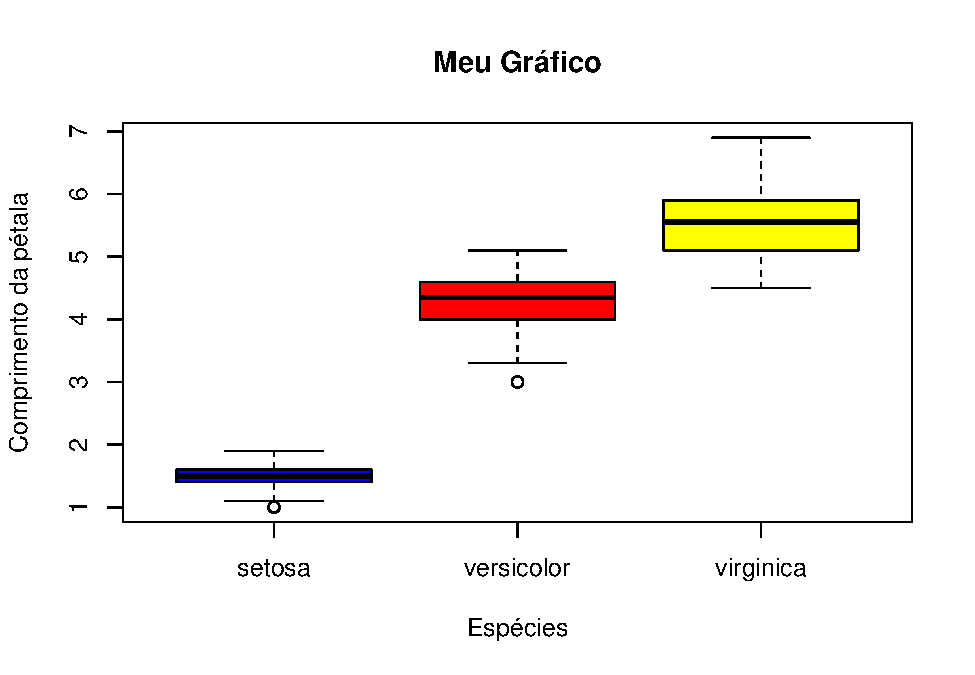
\includegraphics{livroR-1.0_files/figure-latex/unnamed-chunk-37-1} \end{center}

\begin{enumerate}
\def\labelenumi{(\alph{enumi})}
\tightlist
\item
  boxplot(Petal.Length,
  Species,
  data = iris,
  col = c(``blue'', ``red'', ``yellow''),
  xlab = ``Espećies'',
  ylab = ``Comprimento da pétala'',
  main = ``Meu Gráfico'')
\item
  boxplot(Petal.Length \textasciitilde{} Species,
  data = iris,
  col = c(``blue'', ``red'', ``yellow''),
  xlab = ``Espécies'',
  ylab = ``Comprimento da pétala'',
  main = ``Meu Gráfico'')
\item
  boxplot(``Petal.Length'' \textasciitilde{} ``Species'',
  data = ``iris'',
  col = c(``blue'', ``red'', ``yellow''),
  xlab = ``Espécies'',
  ylab = ``Comprimento da pétala'',
  main = ``Meu Gráfico'')
\item
  boxplot(Petal.Length \textasciitilde{} Species,
  data = iris,
  col = c(blue, red, yellow),
  xlab = ``Espécies'',
  ylab = ``Comprimento da pétala'',
  main = ``Meu Gráfico'')
\item
  boxplot(Petal.Length \textasciitilde{} Species,
  data = iris,
  col = c(``azul'', ``vermelho'', ``amarelo''),
  xlab = ``Espécies'',
  ylab = ``Comprimento da pétala'',
  main = ``Meu Gráfico'')
\end{enumerate}

\begin{enumerate}
\def\labelenumi{\arabic{enumi})}
\setcounter{enumi}{4}
\tightlist
\item
  Execute os seguintes comandos no seu R: set.seed(458); teste \textless{}- rnorm(100, sd = 0.2). Qual das opções abaixo representam, na ordem, a média, mediana, desvio padrão, variância e amplitude destes dados.
\end{enumerate}

\begin{enumerate}
\def\labelenumi{(\alph{enumi})}
\tightlist
\item
  0,01; 0,02; 0,12; 0,04; 1,24
\item
  0,02; 0,01; 0,21; 1,24; 0,04
\item
  0,02; 0,01; 0,21; 0,04; 1,24
\item
  0,01; 0,02; 0,12; 0,04; 1,24
\item
  0,02; 0,01; 0,31; 0,04; 1,20
\end{enumerate}

\hypertarget{qui-quadrado-chi}{%
\chapter{\texorpdfstring{Qui-quadrado (\(\chi\)²)}{Qui-quadrado (\textbackslash{}chi²)}}\label{qui-quadrado-chi}}

Até o momento aprendemos a definir o ambiente em que iremos trabalhar, importar nossa planilha, verifica-la e ajusta-la se necessário, assim como as métricas mais utilizadas para sumarizar os dados. Mas por vezes estamos interessados em analisar os dados, então vamos começar com o Qui-quadrado.

Em alguns momentos podemos estar trabalhando com variáveis categóricas e lidarmos com perguntas sobre estas variáveis e portanto pode ser necessário avaliarmos se a frequência das observações de uma dada variável categórica ajusta-se ao que se é esperado (\(\chi\)² para ajuste de frequências) ou se as proporções das observações de duas ou mais variáveis categóricas são independentes uma da outra (\(\chi\)² para independência).

De modo que, para este teste iremos precisar apenas de uma variável (se estivermos avaliando o ajuste de frequências) ou duas variáveis (se avaliarmos a independência) e estas devem ser categóricas. Como aprendemos anteriormente as variáveis categóricas devem ser classificadas como fator (pela função \textcolor{blue}{as.factor()}) no R. Vamos conferir em detalhes e com exemplos como realizar estas duas análises no R.

\hypertarget{chi-para-ajuste-de-frequuxeancias}{%
\section{\texorpdfstring{\(\chi\)² para ajuste de frequências}{\textbackslash{}chi² para ajuste de frequências}}\label{chi-para-ajuste-de-frequuxeancias}}

\begin{table}

\caption{\label{tab:tab1qui}Principais características do qui-quadrado para ajuste das frequências}
\centering
\begin{tabular}[c]{>{\raggedright\arraybackslash}p{10em}>{\raggedright\arraybackslash}p{30em}}
\toprule
Atributos & Características\\
\midrule
\textbf{\cellcolor{gray!6}{Tipo de variável}} & \cellcolor{gray!6}{Categórica}\\
\textbf{Quantidade de variáveis} & 1\\
\textbf{\cellcolor{gray!6}{Hipótese nula}} & \cellcolor{gray!6}{O número de observações em cada grupo da variável é similar ao predito pela teoria}\\
\textbf{Fórmula} & $$\chi^2=\sum^{N}_{i = 1}\frac{(Ob-Es)^2}{Es}$$\\
\textbf{\cellcolor{gray!6}{Observação}} & \cellcolor{gray!6}{Se há apenas 2 categorias, dentro da variável, não há a necessidade de post-hoc nem expressa-la graficamente}\\
\bottomrule
\end{tabular}
\end{table}

Imagine o seguinte exemplo: Você foi a praia e verificou uma enorme quantidade de produtos plásticos, esquecidos pelas pessoas. Após um tempo de observação você percebeu que haviam tanto sacolas quanto tampas de garrafa PET e poderia levantr a seguinte pergunta: Será que se coletarmos estes plásticos na praia e o categorizarmos eles apresentarão quantidades similares? A partir desta pergunta a seguinte hipótese nula (H0) é naturalmente construída: Não há diferenças entre estes dois tipos de plásticos (tampas e sacolas). O \(\chi\)² objetiva responder a essa pergunta e fornecer subsídio estatístico para corroborar ou refutar essa hipótese.

Após a observação, coleta, classificação e contagem dos fragmentos plásticos os seguintes valores foram observados: 520 sacolas plásticas e 470 tampas. Dessa forma podemos perguntar: do total de fragmentos coletados (520 para sacolas e 470 para tampas) cada um deles contribuem com 50\% (percentuais iguais) do total?

Vamos começar criando 2 vetores\footnote{Vetores é uma estrutura básica do R que consiste em um objeto que contêm elementos de mesma classe. Se realizarmos o comando \textcolor{green}{c(1, 2, 3)}, criamos um vetor, mas não um objeto. Se criarmos o seguinte: \textcolor{green}{teste <- c(1, 2, 3)} estaremos criando um objeto do tipo vetor.} onde o primeiro corresponde aos valores observados e o segundo as proporções esperadas para cada valor.

\begin{Shaded}
\begin{Highlighting}[]
\NormalTok{observados <-}\StringTok{ }\KeywordTok{c}\NormalTok{(}\DecValTok{520}\NormalTok{, }\DecValTok{470}\NormalTok{)}
\NormalTok{esperados <-}\StringTok{ }\KeywordTok{c}\NormalTok{(}\FloatTok{0.5}\NormalTok{, }\FloatTok{0.5}\NormalTok{)}

\NormalTok{observados}
\end{Highlighting}
\end{Shaded}

\begin{verbatim}
## [1] 520 470
\end{verbatim}

\begin{Shaded}
\begin{Highlighting}[]
\NormalTok{esperados}
\end{Highlighting}
\end{Shaded}

\begin{verbatim}
## [1] 0.5 0.5
\end{verbatim}

Note que criamos os objetos ``observados'' e ``esperados''. O primeiro corresponde ao que coletamos e o segundo as proporções que esperamos de ambos.

Para realizar o teste do \(\chi\)² para ajuste de frequências, vamos utilizar a função \textcolor{blue}{chisq.test()}.

\begin{Shaded}
\begin{Highlighting}[]
\KeywordTok{chisq.test}\NormalTok{(}\DataTypeTok{x =}\NormalTok{ observados, }\DataTypeTok{p =}\NormalTok{ esperados)}
\end{Highlighting}
\end{Shaded}

\begin{verbatim}
## 
##  Chi-squared test for given probabilities
## 
## data:  observados
## X-squared = 2.5253, df = 1, p-value = 0.112
\end{verbatim}

Esta função utiliza 2 argumentos:
* x: no qual inserimos o vetor númerico que contém os valores referentes a quantidade da variável nominal que contabilizamos;
* p: no qual inserimos o vetor númerico que contem as proporções esperadas associado a cada grupo da categoria avaliada.

Note que o resultado indica o teste realizado, o nome do objeto que contém os dados e na terceira linha ele apresenta o resultado como valor do teste do \(\chi\)², o grau de liberdade (\emph{df} do inglês \emph{degrees of freedom}) e o valor de probabilidade associado (do inglês \emph{p-value}).

Uma característica do \(\chi\)² é que quanto mais similares forem os valores observados menor será o valor do \(\chi\)², mas nunca menor que 0 e com o \emph{p-value} máximo igual a 1 e quanto mais dissimilares forem os valores observados maior será o \(\chi\)² (tendendo a infinito) e menor será o \emph{p-value} (tendendo a 0)

Com isso podemos observar que o \(\chi\)² varia entre (0 e + infinito) enquanto que o \emph{p-value} varia entre (0 e 1) com uma relação inversa entre eles. Quanto maior o \(\chi\)² menor o \emph{p-value} e quanto menor o \(\chi\)² maior o \emph{p-value}.

Por convenção indicamos que um teste estatístico que apresenta \emph{p-value} \textless{} 0,05 indica diferenças significativas entre os valores observados. Dessa forma, assumindo essa convenção, podemos concluir que a quantidade de sacolas não difere da quantidade de tampas de garrafa PET. Portanto aceitamos a hipótese nula.

Não é comum representar o resultado deste teste graficamente apenas como valor mas se mesmo assim quiser representa-lo utilize um gráfico de barras.

Vamos verificar outros exemplos e avaliar suas hipóteses nulas.

Imagine um segundo exemplo. 300 flores foram fotografadas e classificadas pela cor e ao final foi obtido um total de 170 flores vermelhas e 130 flores verdes. Ao ler alguns trabalhos e analisar os resultados observados para outra região foi levantada a hipótese de que 70\% das flores seriam vermelhas e 30\% seriam verdes. Com base nesses dados podemos perguntar: As flores fotografadas confirmam os resultados esperados?

Vamos avaliar este caso, conforme fizemos acima.

\begin{Shaded}
\begin{Highlighting}[]
\NormalTok{flores.observadas <-}\StringTok{ }\KeywordTok{c}\NormalTok{(}\DecValTok{170}\NormalTok{, }\DecValTok{130}\NormalTok{)}
\NormalTok{flores.esperadas <-}\StringTok{ }\KeywordTok{c}\NormalTok{(}\FloatTok{0.7}\NormalTok{, }\FloatTok{0.3}\NormalTok{)}
\end{Highlighting}
\end{Shaded}

Observe que igual nosso exemplo anterior criamos objetos \textbf{flores.observadas} e \textbf{flores.esperadas}. Note que a diferença está nos valores esperados, onde alteramos a proporção, que não é mais de 50\% para cada, mas sim de 70\% para um e 30\% para outro, porém expressos em proporção (valores variam entre 0 e 1). Perceba, também, que os valores seguem a ordem em que foram inseridos, portanto o primeiro valor observado inserido corresponde ao primeiro valor esperado inserido e assim por diante.

Ao conduzir a análise temos o seguinte resultado

\begin{Shaded}
\begin{Highlighting}[]
\KeywordTok{chisq.test}\NormalTok{(}\DataTypeTok{x =}\NormalTok{ flores.observadas, }\DataTypeTok{p =}\NormalTok{ flores.esperadas)}
\end{Highlighting}
\end{Shaded}

\begin{verbatim}
## 
##  Chi-squared test for given probabilities
## 
## data:  flores.observadas
## X-squared = 25.397, df = 1, p-value = 4.667e-07
\end{verbatim}

Perceba que o valor do \(\chi\)² aumentou em relação ao exemplo anterior e o \emph{p-value} diminuiu para um valor bem próximo a 0. Este resultado indica que os valores observados de flores vermelhas e verdes não apresentam as proporções que se esperam de 70\% e 30\%. Portanto refutamos a hipótese nula de que elas se encontram nas proporções esperadas.

Vamos seguir em frente e olhar para um outro exemplo. Suponha que foram coletados 2660 indivíduos de siri em um estuário. Eles foram classificados em relação ao sexo e foram obtidos 1380 fêmeas e 1280 machos. Espera-se que a razão sexual desta espécie seja de 1:1 (50\% para cada sexo). Os indivíduos amostrados confirmam o que é esperado?

\begin{Shaded}
\begin{Highlighting}[]
\NormalTok{siris.observados <-}\StringTok{ }\KeywordTok{c}\NormalTok{(}\DecValTok{1380}\NormalTok{, }\DecValTok{1280}\NormalTok{)}
\NormalTok{siris.esperados <-}\StringTok{ }\KeywordTok{c}\NormalTok{(}\FloatTok{0.5}\NormalTok{, }\FloatTok{0.5}\NormalTok{)}

\KeywordTok{chisq.test}\NormalTok{(}\DataTypeTok{x =}\NormalTok{ siris.observados, }\DataTypeTok{p =}\NormalTok{ siris.esperados)}
\end{Highlighting}
\end{Shaded}

\begin{verbatim}
## 
##  Chi-squared test for given probabilities
## 
## data:  siris.observados
## X-squared = 3.7594, df = 1, p-value = 0.05251
\end{verbatim}

Com este caso podemos observar que o valor do \(\chi\)² indicou um \emph{p-value} próximo a 0,05, indicando que temos de ter cuidado com as afirmações relativas a hipótese testada. Contudo, como o valor é \textgreater{}0,5 podemos corroborar a hipotese nula e dizer que os valores observados para fêmeas e machos encontram-se dentro da proporção esperada de 1:1.

E se ao invés de 2 grupos tivessemos 3 ou mais. Como realizariamos o \(\chi\)²? Vamos ver com um exemplo.

Imagine que você foi a uma floresta e classificou as árvores em altas, médias e baixas e contabilizou 55, 31 e 27 respectivamente. De acordo com a literatura é esperado que as proporções de árvores altas, médias e baixas seja de 1:1:1. Vamos analisar e verificar se podemos afirmar que o observado corrobora o esperado.

\begin{Shaded}
\begin{Highlighting}[]
\NormalTok{arvores.observadas <-}\StringTok{ }\KeywordTok{c}\NormalTok{(}\DecValTok{55}\NormalTok{, }\DecValTok{31}\NormalTok{, }\DecValTok{27}\NormalTok{)}
\NormalTok{arvores.esperadas <-}\StringTok{ }\KeywordTok{c}\NormalTok{(}\DecValTok{1}\OperatorTok{/}\DecValTok{3}\NormalTok{, }\DecValTok{1}\OperatorTok{/}\DecValTok{3}\NormalTok{, }\DecValTok{1}\OperatorTok{/}\DecValTok{3}\NormalTok{)}

\KeywordTok{chisq.test}\NormalTok{(}\DataTypeTok{x =}\NormalTok{ arvores.observadas, }\DataTypeTok{p =}\NormalTok{ arvores.esperadas)}
\end{Highlighting}
\end{Shaded}

\begin{verbatim}
## 
##  Chi-squared test for given probabilities
## 
## data:  arvores.observadas
## X-squared = 12.177, df = 2, p-value = 0.002269
\end{verbatim}

Neste exemplo podemos perceber que a análise é igual a todos os casos anteriores, a diferença é que adicionamos um grupo a mais e consequentemente um valor a mais. Devido a essa mudança tivemos que dividir as probabilidades (objeto \textbf{arvores.esperadas}) em 3 valores e de igual probabilidade, já que o hipotetizado consistia em proporções iguais para os três grupos definidos. De acordo com o resultado obtido podemos perceber que o que foi observado não corrobora o esperado.

Vamos observar quais seriam as quantidades de árvores esperadas de acordo com as quantidades que observamos e as proporções que esperamos.

Para isso precisamos primeiramente inserir o resultado em um objeto e a seguir acessar os componentes desse objeto pelo operador matemático \textbf{\$} (cifrão), seguido pelo objeto \textbf{expected} criado pela função \textcolor{blue}{chisq.test()}.

\begin{Shaded}
\begin{Highlighting}[]
\NormalTok{resultado <-}\StringTok{ }\KeywordTok{chisq.test}\NormalTok{(}\DataTypeTok{x =}\NormalTok{ arvores.observadas, }\DataTypeTok{p =}\NormalTok{ arvores.esperadas)}

\NormalTok{resultado}\OperatorTok{$}\NormalTok{expected}
\end{Highlighting}
\end{Shaded}

\begin{verbatim}
## [1] 37.66667 37.66667 37.66667
\end{verbatim}

Os exemplos acima tratam de avaliar o \(\chi\)² em variáveis que apresentam dois ou mais grupos. Quando o grau de liberdade é 1 (dois grupos) e o número de observações é considerado baixo é sugerido a aplicação da correção de Yates. Quando o número de observações é elevado ela não distorce o resultado. O risco de se usar o \(\chi\)² sem a correção de Yates consiste em inflar o valor de \(\chi\)² e portanto diminuir o \emph{p-value} o que nos levaria ao risco de rejeitarmos a hipótese nula quando ela é verdadeira (erro tipo I).

A função do \(\chi\)², no pacote base do R, não realiza a correção de Yates para este teste, apenas para o próximo caso que iremos tratar (\(\chi\)² para independência). Contudo ele oferece outro método para avaliação deste teste que consiste na simulação de Monte Carlo. Não entraremos em detalhes de como funciona este teste, mas o que alertamos é que se o número de observações utilizado é considerado baixo correções devem ser aplicadas. Embora os cálculos envolvidos para realização da correção de Yates não seja complicada sugerimos a leitura da literatura especializada.

Vamos verificar um exemplo onde a correção de Monte Carlo, a qual é possível de ser realizada de maneira rápida e prática no R, é aplicada.

Imagine que você foi em campo e contabilizou as espécies de cracas que identificou. Foram contabilizados 12 cracas da espécie A e 24 da espécie B. Trabalhos anteriores demonstraram que ambas as espécies encontram-se na proporção de 1:1. Aplicando a simulação de Monte Carlo o número de indivíduos observados de ambas as espécies corroboram o esperado?

\begin{Shaded}
\begin{Highlighting}[]
\NormalTok{N.especies <-}\StringTok{ }\KeywordTok{c}\NormalTok{(}\DecValTok{12}\NormalTok{, }\DecValTok{24}\NormalTok{)}
\NormalTok{prop.especies <-}\StringTok{ }\KeywordTok{c}\NormalTok{(}\FloatTok{0.5}\NormalTok{, }\FloatTok{0.5}\NormalTok{)}

\KeywordTok{chisq.test}\NormalTok{(}\DataTypeTok{x =}\NormalTok{ N.especies, }\DataTypeTok{p =}\NormalTok{ prop.especies, }\DataTypeTok{simulate.p.value =} \OtherTok{FALSE}\NormalTok{)}
\end{Highlighting}
\end{Shaded}

\begin{verbatim}
## 
##  Chi-squared test for given probabilities
## 
## data:  N.especies
## X-squared = 4, df = 1, p-value = 0.0455
\end{verbatim}

\begin{Shaded}
\begin{Highlighting}[]
\KeywordTok{chisq.test}\NormalTok{(}\DataTypeTok{x =}\NormalTok{ N.especies, }\DataTypeTok{p =}\NormalTok{ prop.especies, }\DataTypeTok{simulate.p.value =} \OtherTok{TRUE}\NormalTok{)}
\end{Highlighting}
\end{Shaded}

\begin{verbatim}
## 
##  Chi-squared test for given probabilities with simulated p-value (based
##  on 2000 replicates)
## 
## data:  N.especies
## X-squared = 4, df = NA, p-value = 0.07146
\end{verbatim}

Basta usarmos o argumento ``simulate.p.value'' e indicar ``FALSE'' quando não queremos a simulação de Monte Carlo, ou apenas omitirmos este argumento, ou usar este argumento e indicar ``TRUE'' o qual realiza a simulação de Monte Carlo. Verifique que com a aplicação desta simulação o \emph{p-value} aumenta indicando que torna mais dificil rejeitarmos a hipótese nula. Após aplicarmos a correção na nossa análise podemos afirmar que não há diferença na quantidade de cracas observadas em relação as proporções esperadas, para ambas as espécies de cracas.

Relembrando. Sempre tome cuidado com afirmações! Principalmente quando o número de observações é baixo. Mesmo que o teste estatístico indique diferenças, uma baixa quantidade de observações devem ser analisadas cuidadosamente, no entanto devemos aplicar correções matemáticas nestes casos.

\hypertarget{chi-para-independuxeancia}{%
\section{\texorpdfstring{\(\chi\)² para independência}{\textbackslash{}chi² para independência}}\label{chi-para-independuxeancia}}

Realizamos este teste quando objetivamos saber se a frequência dos grupos de uma variável é independente de outra variável.

Diferente do primeiro caso de \(\chi\)² que abordamos, este lida com duas variáveis categóricas ao invés de uma. Portanto é necessário o desenvolvimento de uma tabela de contigência.

A tabela de contigência consiste em uma tabela com o número de observações referentes as duas variáveis selecionadas. Veremos alguns exemplos abaixo.

Para o momento. Veja o sumário abaixo no qual detalhamos as principais características desta análise.

\begin{table}

\caption{\label{tab:tab2qui}Principais características do qui-quadrado para independência}
\centering
\begin{tabular}[c]{>{\raggedright\arraybackslash}p{10em}>{\raggedright\arraybackslash}p{30em}}
\toprule
Atributos & Características\\
\midrule
\textbf{\cellcolor{gray!6}{Tipo de variável}} & \cellcolor{gray!6}{Categórica.}\\
\textbf{Quantidade de variáveis} & 2 ou mais.\\
\textbf{\cellcolor{gray!6}{Hipótese nula}} & \cellcolor{gray!6}{As proporções relativas de uma variável são independentes de uma segunda variável.}\\
\textbf{Fórmula} & Para uma tabela 2 $\times$2 temos: $$\chi^{2} = \frac{n(f_{11}f_{22}-f_{12}f_{21})^2}{R_{1}R_{2}C_{1}C_{2}}$$ Onde n é onúmero total de observações; $f_{11}$ é o valor da primeira linha e primeira coluna; $f_{22}$ é o valor da segunda linha e segunda coluna; $f_{12}$ é o valor da primeira linha e da segunda coluna; $f_{21}$ é o valor da segunda linha e primeira coluna; $R_{1}$ é a soma da primeira linha; $R_{2}$ é a soma da segunda linha; $C_{1}$ é a soma da primeira coluna e $C_{2}$ é a soma da segunda coluna.\\
\textbf{\cellcolor{gray!6}{Observação}} & \cellcolor{gray!6}{Como característica intrinseca a este teste é necessário a construção da tabela de contigência.}\\
\bottomrule
\end{tabular}
\end{table}

Imagine a seguinte situação: Insetos foram coletados, ao acaso, em uma região costeira. Todos os insetos foram avaliados quanto a espécie e a presença de parasitas. Os seguintes valores foram obtidos: 55 indivíduos da espécie A com parasita, 75 indivíduos da espécie A sem parasita, 90 indivíduos da espécie B com parasita e 110 indivíduos da espécie B sem parasita. Foi levantada a hipótese nula de que a quantidade de indivíduos infectados pelo parasita é o mesmo para ambas as espécies.

Vamos começar criando uma matriz\footnote{É um conjunto de elementos com estrutura n-dimensional, ou seja, com várias linhas e colunas, onde todos os seus elementos são de mesmo tipo (númerico, inteiro, fator, caracter etc).} com esses valores, onde as linhas corresponderão as espécies, as colunas a presença/ausência do parasita e os seus elementos corresponderão a quantidade de indivíduos dada as condições (espécie e parasita).

Para construir nossos dados utilizaremos a função \textcolor{blue}{matrix}, com os argumentos ``data'', onde adicionaremos os elementos que estarão presentes, ``ncol'' onde definiremos a quantidade de colunas e ``byrow'' onde definiremos que os valores presentes no argumento ``data'' serão inseridos em ordem por linha, neste caso a função começará preenchendo a primeira linha da primeira coluna, segunda linha da primeira coluna, primeira linha da segunda coluna e segunda linha da segunda coluna. Guardaremos nossa matriz criada em um objeto chamado \textbf{dados}. Utilizaremos as funções \textcolor{blue}{rownames()} e \textcolor{blue}{colnames()} a fim de definir os nomes das linhas e colunas da nossa matriz para melhor visualização. A seguir iremos visualizar o objeto \textbf{dados}.

\begin{Shaded}
\begin{Highlighting}[]
\NormalTok{dados <-}\StringTok{ }\KeywordTok{matrix}\NormalTok{(}\DataTypeTok{data =} \KeywordTok{c}\NormalTok{(}\DecValTok{55}\NormalTok{, }\DecValTok{75}\NormalTok{, }\DecValTok{90}\NormalTok{, }\DecValTok{110}\NormalTok{), }\DataTypeTok{ncol =} \DecValTok{2}\NormalTok{, }\DataTypeTok{byrow =} \OtherTok{TRUE}\NormalTok{)}
\KeywordTok{rownames}\NormalTok{(dados) <-}\StringTok{ }\KeywordTok{c}\NormalTok{(}\StringTok{"Espécie A"}\NormalTok{, }\StringTok{"Espécie B"}\NormalTok{)}
\KeywordTok{colnames}\NormalTok{(dados) <-}\StringTok{ }\KeywordTok{c}\NormalTok{(}\StringTok{"Com parasita"}\NormalTok{, }\StringTok{"Sem parasita"}\NormalTok{)}
\NormalTok{dados}
\end{Highlighting}
\end{Shaded}

\begin{verbatim}
##           Com parasita Sem parasita
## Espécie A           55           75
## Espécie B           90          110
\end{verbatim}

Pronto nossa tabela de contigência está criada. Vamos seguir para a análise

\begin{Shaded}
\begin{Highlighting}[]
\KeywordTok{chisq.test}\NormalTok{(}\DataTypeTok{x =}\NormalTok{ dados)}
\end{Highlighting}
\end{Shaded}

\begin{verbatim}
## 
##  Pearson's Chi-squared test with Yates' continuity correction
## 
## data:  dados
## X-squared = 0.13543, df = 1, p-value = 0.7129
\end{verbatim}

Ao executarmos a função \textcolor{blue}{chisq.test()} utilizando apenas a matriz como objeto do argumento ``x'' ele nos retorna o \(\chi\)² com a correção de Yates. O que é sugerido para quando estamos lidando com matrizes \(2 \times 2\). No geral o resultado é similar ao que executamos no tópico anterior.

Uma atenção deve ser dada ao grau de liberdade o qual indica o valor de 1. O cálculo do grau de liberdade consiste no número de linhas menos um multiplicado pelo número de colunas menos um. Como temos 2 linhas e 2 colunas o grau de liberdade será: \((2-1)*(2-1) = 1*1 = 1\).

De acordo com o resultado obtido pelo teste não podemos refutar nossa hipótese nula. Portanto dizemos que a proporção da população infectada pelo parasita é a mesma nas duas espécies.

Vejamos um segundo exemplo.

Durante 2 anos camarões foram coletados, em um estuário, e todos eles foram sexados em machos e fêmeas. Objetivou-se com esses dados saber se há algum desvio da razão sexual entre os anos.

Vamos começar desenvolvendo um conjunto de dados na forma de planilha, que é como seus dados devem estar planilhados e vamos ensina-lo a construir uma tabela de contingência a partir desses dados.

Execute o código abaixo. Não se preocupe, no momento, com as funções novas utilizadas. A única função diferente é \textcolor{blue}{rep()} que repete um determinado elemento n vezes. No código abaixo, estaremos repetindo o elemento ``Ano 1'' 150 vezes e o elemento ``Ano 2'' 225 vezes e concatenaremos estes elementos por meio da função \textcolor{blue}{c()} e guardando-o no objeto \textbf{ano} faremos o mesmo para o objeto \textbf{sexo} onde concatenaremos a repetição do elemento ``macho'' 55 vezes, seguido por ``fêmea'' 95 vezes, seguido novamente por ``macho'' 105 vezes e por fim ``fêmea'' 120 vezes. Após isso uniremos os dois objetos \textbf{ano} e \textbf{sexo} por meio da função \textcolor{blue}{cbind()} e diremos que isso consiste em um objeto da classe \emph{data frame} por meio da função \textcolor{blue}{data.frame()} e guardaremos esse resultado em um objeto denominado \textbf{dados}.

\begin{Shaded}
\begin{Highlighting}[]
\NormalTok{ano <-}\StringTok{ }\KeywordTok{c}\NormalTok{(}\KeywordTok{rep}\NormalTok{(}\StringTok{"Ano 1"}\NormalTok{, }\DecValTok{150}\NormalTok{), }\KeywordTok{rep}\NormalTok{(}\StringTok{"Ano 2"}\NormalTok{, }\DecValTok{225}\NormalTok{))}
\NormalTok{sexo <-}\StringTok{ }\KeywordTok{c}\NormalTok{(}\KeywordTok{rep}\NormalTok{(}\StringTok{"macho"}\NormalTok{, }\DecValTok{55}\NormalTok{), }\KeywordTok{rep}\NormalTok{(}\StringTok{"fêmea", 95), rep("}\NormalTok{macho}\StringTok{", 105), rep("}\NormalTok{fêmea", }\DecValTok{120}\NormalTok{))}

\NormalTok{dados <-}\StringTok{ }\KeywordTok{data.frame}\NormalTok{(}\KeywordTok{cbind}\NormalTok{(ano, sexo))}
\end{Highlighting}
\end{Shaded}

Vamos visualizar nossos dados. Para isso podemos usar a função \textcolor{blue}{head()} que mostra no console as primeiras linhas desse \emph{data frame}.

\begin{Shaded}
\begin{Highlighting}[]
\KeywordTok{head}\NormalTok{(dados)}
\end{Highlighting}
\end{Shaded}

\begin{verbatim}
##     ano  sexo
## 1 Ano 1 macho
## 2 Ano 1 macho
## 3 Ano 1 macho
## 4 Ano 1 macho
## 5 Ano 1 macho
## 6 Ano 1 macho
\end{verbatim}

Agora vamos, a partir de \textbf{dados} construir uma tabela de contigência. Para isso vamos utilizar a função \textcolor{blue}{table()} e guardar seu resultado em um objeto chamado \textbf{tab.cont}. A seguir iremos visualizar nossa tabela de contingência chamando \textbf{tab.cont}

\begin{Shaded}
\begin{Highlighting}[]
\NormalTok{tab.cont <-}\StringTok{ }\KeywordTok{table}\NormalTok{(dados)}
\NormalTok{tab.cont}
\end{Highlighting}
\end{Shaded}

\begin{verbatim}
##        sexo
## ano     fêmea macho
##   Ano 1    95    55
##   Ano 2   120   105
\end{verbatim}

Vamos agora realizar o qui-quadrado de nossos dados.

\begin{Shaded}
\begin{Highlighting}[]
\KeywordTok{chisq.test}\NormalTok{(tab.cont)}
\end{Highlighting}
\end{Shaded}

\begin{verbatim}
## 
##  Pearson's Chi-squared test with Yates' continuity correction
## 
## data:  tab.cont
## X-squared = 3.2817, df = 1, p-value = 0.07006
\end{verbatim}

Pronto! Como podem ver, a representação do resultado é similar ao exemplo acima. Contudo nossos dados são diferentes e portanto nossa hipótese nula é diferente.

Nossa hipótese nula pode ser escrita de três formas. Vejamos os 3 exemplos abaixo:

\begin{itemize}
\tightlist
\item
  H0: Na população amostrada a proporção de machos e fêmeas é independente do ano;
\item
  H0: Na população amostrada a razão sexual dos camarões é a mesma entre os anos;
\item
  H0: A proporção de camarões entre os anos é a mesma para ambos os sexos;
\end{itemize}

Como o teste resultou em um \emph{p-value} maior que 0,05 podemos dizer, por essa via, que corroboramos nossa hipótese nula.

Neste ponto é bom relembramos da importância do número de observações de cada grupo. Se este número for pequeno, incertezas podem ser geradas e ajustes devem ser feitos. Contudo, para definir o que é um número baixo de observações sigamos para o cálculo sugerido por Zar (2010)\footnote{Zar, J. H. (2010). Biostatistical analysis (5th ed.). Upper Saddle River, N.J.: Prentice-Hall/Pearson.} o qual define como: \(n = 6rc\).

Onde, n é o número de observações mínimo de cada grupo, r é o número de linhas (\emph{rows}) e c é o número de colunas (\emph{column}). Dessa forma, em uma tabela de contigência do tipo \(2 \times 2\) o número de observações mínimo para cada grupo deve ser de: \(n = 6 \times (2) \times (2) = 24\). Ou seja, 24 observações.

Esta análise pode ser conduzida, também, quando lidamos com mais de um grupo em uma categoria e neste caso teriamos uma tabela de contigência \(2 \times 3\), \(2 \times 4\), \(3 \times 3\) e assim por diante. Vamos ver um exemplo.

Três pesquisadores analisaram fotografias de espécies bentônicas em um costão objetivando avaliar a abundância de duas espécies, uma introduzida e uma nativa. Considere todo o processo amostral similar e que os pesquisadores avaliaram as mesmas fotografias. Neste caso nossa hipótese nula é que a proporção entre as espécies é similar independentemente dos pesquisadores.

Vamos construir nossa matriz de uma outra forma.

\begin{Shaded}
\begin{Highlighting}[]
\NormalTok{pesquisadores <-}\StringTok{ }\KeywordTok{c}\NormalTok{(}\StringTok{"pesquisador 1"}\NormalTok{, }\StringTok{"pesquisador 2"}\NormalTok{, }\StringTok{"pesquisador 3"}\NormalTok{)}
\NormalTok{sp.nativa <-}\StringTok{ }\KeywordTok{c}\NormalTok{(}\DecValTok{70}\NormalTok{, }\DecValTok{79}\NormalTok{, }\DecValTok{38}\NormalTok{)}
\NormalTok{sp.introduzida <-}\StringTok{ }\KeywordTok{c}\NormalTok{(}\DecValTok{84}\NormalTok{, }\DecValTok{95}\NormalTok{, }\DecValTok{80}\NormalTok{)}
\NormalTok{dados <-}\StringTok{ }\KeywordTok{matrix}\NormalTok{(}\KeywordTok{c}\NormalTok{(sp.nativa, sp.introduzida), }\DataTypeTok{nrow =} \DecValTok{2}\NormalTok{, }\DataTypeTok{byrow =}\NormalTok{ T)}
\KeywordTok{colnames}\NormalTok{(dados) <-}\StringTok{ }\NormalTok{pesquisadores}
\KeywordTok{rownames}\NormalTok{(dados) <-}\StringTok{ }\KeywordTok{c}\NormalTok{(}\StringTok{"Espécie nativa"}\NormalTok{, }\StringTok{"Espécie introduzida"}\NormalTok{)}
\NormalTok{dados}
\end{Highlighting}
\end{Shaded}

\begin{verbatim}
##                     pesquisador 1 pesquisador 2 pesquisador 3
## Espécie nativa                 70            79            38
## Espécie introduzida            84            95            80
\end{verbatim}

Os dados foram construídos passo a passo. Vamos analisar e verificar o resultado.

\begin{Shaded}
\begin{Highlighting}[]
\KeywordTok{chisq.test}\NormalTok{(dados)}
\end{Highlighting}
\end{Shaded}

\begin{verbatim}
## 
##  Pearson's Chi-squared test
## 
## data:  dados
## X-squared = 6.2322, df = 2, p-value = 0.04433
\end{verbatim}

Repare que há algo diferente, como realizamos a análise em uma tabela \(2 \times 3\) por padrão a função \textcolor{blue}{chisq.test()} não realiza a correção de Yates. Pois não é necessário.

Analisando o resultado podemos inferir que as proporções observadas de espécies nativas e introduzidas são diferentes em função do pesquisador. Ou seja, rejeitamos nossa hipótese nula de que as proporções são similares. Contudo o \emph{p-value} foi bem próximo ao limiar de 0,05. Podemos nos aprofundar na questão e nos perguntar onde está essa diferença? Entre o pesquisador 1 e o pesquisador 2 ou entre outra dupla de pesquisadores? Como observamos isso?

Para responder essa pergunta em específico, vamos subdividir nossa tabela de contigência para todos os pares de observações e armazena-los em outros objetos.

Para isso criaremos tabelas \(2 \times 2\) para cada par de comparações. Repare que usaremos a nossa tabela \textbf{dados} originalmente criada seguida por colchetes e dentro do colchetes inserimos virgula e menos o número referente a coluna. O colchetes após o nome dos dados nos permite acessar as linhas e colunas de um conjunto de dados quaisquer com isso podemos remove-las ou seleciona-las. Qualquer número antes da virgula indica a linha e qualquer número após a vírgula indica a coluna. O sinal de menos indica que vamos remover e se não colocarmos sinal indica que iremos selecionar o valor especificado. No primeiro caso onde inserimos ``-3'' após a virgula estamos indicando que vamos remover a terceira coluna do objeto dados e armazenar este resultado em um novo objeto chamado \textbf{p1.p2}. O mesmo raciocínio segue nos demais casos.

\begin{Shaded}
\begin{Highlighting}[]
\NormalTok{p1.p2 <-}\StringTok{ }\NormalTok{dados [, }\DecValTok{-3}\NormalTok{]}
\NormalTok{p1.p3 <-}\StringTok{ }\NormalTok{dados [, }\DecValTok{-2}\NormalTok{]}
\NormalTok{p2.p3 <-}\StringTok{ }\NormalTok{dados [, }\DecValTok{-1}\NormalTok{]}
\end{Highlighting}
\end{Shaded}

Sabendo isso vamos realizar a função \textcolor{blue}{chisq.test()} para cada par de observações e analisar seu resultado.

\begin{Shaded}
\begin{Highlighting}[]
\KeywordTok{chisq.test}\NormalTok{(p1.p2)}
\end{Highlighting}
\end{Shaded}

\begin{verbatim}
## 
##  Pearson's Chi-squared test with Yates' continuity correction
## 
## data:  p1.p2
## X-squared = 0, df = 1, p-value = 1
\end{verbatim}

\begin{Shaded}
\begin{Highlighting}[]
\KeywordTok{chisq.test}\NormalTok{(p1.p3)}
\end{Highlighting}
\end{Shaded}

\begin{verbatim}
## 
##  Pearson's Chi-squared test with Yates' continuity correction
## 
## data:  p1.p3
## X-squared = 4.3623, df = 1, p-value = 0.03674
\end{verbatim}

\begin{Shaded}
\begin{Highlighting}[]
\KeywordTok{chisq.test}\NormalTok{(p2.p3)}
\end{Highlighting}
\end{Shaded}

\begin{verbatim}
## 
##  Pearson's Chi-squared test with Yates' continuity correction
## 
## data:  p2.p3
## X-squared = 4.5663, df = 1, p-value = 0.03261
\end{verbatim}

Repare que não há diferenças entre a proporção de espécies observadas entre os pesquisadores 1 e 2. Mas entre o pesquisador 3 e os demais há diferença. Isto indica que é o pesquisador 3 que destoa dos demais em relação a observação de espécies nativas e introduzidas.

Quando observamos todo o conjunto de dados não observamos esta característica, mas ao separarmos os dados a diferença fica evidenciada.

Uma prática comum nesta análise é demonstrar o resultado por meio gráfico. Portanto, vamos observar como representar graficamente este último exemplo.

Primeiro vamos transformar nossa tabela de contigência em uma tabela no qual os valores irão corresponder a proporções relativas. Para isso vamos usar a função \textcolor{blue}{prop.table()} e armazenar este resultado em um objeto chamado \textbf{tabela}.

\begin{Shaded}
\begin{Highlighting}[]
\NormalTok{tabela <-}\StringTok{ }\KeywordTok{prop.table}\NormalTok{(}\DataTypeTok{x =}\NormalTok{ dados)}
\NormalTok{tabela}
\end{Highlighting}
\end{Shaded}

\begin{verbatim}
##                     pesquisador 1 pesquisador 2 pesquisador 3
## Espécie nativa          0.1569507     0.1771300    0.08520179
## Espécie introduzida     0.1883408     0.2130045    0.17937220
\end{verbatim}

Como podem ver o resultado deste nosso passo nos retornou uma tabela de proporções em relação ao total. Podemos transformar-la em percentual, basta multiplicarmos a tabela por 100. Vamos ver o processo

\begin{Shaded}
\begin{Highlighting}[]
\NormalTok{tabela <-}\StringTok{ }\KeywordTok{prop.table}\NormalTok{(}\DataTypeTok{x =}\NormalTok{ dados)}\OperatorTok{*}\DecValTok{100}
\NormalTok{tabela}
\end{Highlighting}
\end{Shaded}

\begin{verbatim}
##                     pesquisador 1 pesquisador 2 pesquisador 3
## Espécie nativa           15.69507      17.71300      8.520179
## Espécie introduzida      18.83408      21.30045     17.937220
\end{verbatim}

Pensando um pouco na nossa análise e no que ela avalia. O \(\chi\)² está avaliando as proporções relativas entre os grupos de uma dada variável, neste último caso a proporção das espécie em relação aos pesquisadores. Então a tabela de proporções ou percentual que nos interessa é a relação entre a espécie nativa e introduzida por pesquisador. A função \textcolor{blue}{prop.table()} nos permite definir isso por meio do argumento ``\emph{margin}'', vamos verificar o resultado olhando para o resultado em percentual.

\begin{Shaded}
\begin{Highlighting}[]
\KeywordTok{prop.table}\NormalTok{(}\DataTypeTok{x =}\NormalTok{ dados, }\DataTypeTok{margin =} \DecValTok{1}\NormalTok{)}\OperatorTok{*}\DecValTok{100}
\end{Highlighting}
\end{Shaded}

\begin{verbatim}
##                     pesquisador 1 pesquisador 2 pesquisador 3
## Espécie nativa           37.43316      42.24599      20.32086
## Espécie introduzida      32.43243      36.67954      30.88803
\end{verbatim}

\begin{Shaded}
\begin{Highlighting}[]
\KeywordTok{prop.table}\NormalTok{(}\DataTypeTok{x =}\NormalTok{ dados, }\DataTypeTok{margin =} \DecValTok{2}\NormalTok{)}\OperatorTok{*}\DecValTok{100}
\end{Highlighting}
\end{Shaded}

\begin{verbatim}
##                     pesquisador 1 pesquisador 2 pesquisador 3
## Espécie nativa           45.45455       45.4023      32.20339
## Espécie introduzida      54.54545       54.5977      67.79661
\end{verbatim}

Como podem visualizar, se usarmos ``\emph{margin} = 1'' ele nos retorna os valores em função das linhas (espécies), se utilizarmos ``\emph{margin} = 2'' ele nos retorna os valores em função das colunas (pesquisadores).

Vamos utilizar ``\emph{margin} = 2'' para construir nossa tabela e plotarmos nosso gráfico (Figura \ref{fig:bar-tab}).

\begin{Shaded}
\begin{Highlighting}[]
\NormalTok{tabela <-}\StringTok{ }\KeywordTok{prop.table}\NormalTok{(}\DataTypeTok{x =}\NormalTok{ dados, }\DataTypeTok{margin =} \DecValTok{2}\NormalTok{)}\OperatorTok{*}\DecValTok{100}
\KeywordTok{par}\NormalTok{(}\DataTypeTok{mar =} \KeywordTok{c}\NormalTok{(}\DecValTok{4}\NormalTok{, }\DecValTok{4}\NormalTok{, }\DecValTok{4}\NormalTok{, }\DecValTok{13}\NormalTok{))}
\KeywordTok{barplot}\NormalTok{(tabela, }
        \DataTypeTok{xlab =} \StringTok{"Percentual de espécies"}\NormalTok{,}
        \DataTypeTok{col =} \KeywordTok{c}\NormalTok{(}\StringTok{"red"}\NormalTok{, }\StringTok{"darkblue"}\NormalTok{), }
        \DataTypeTok{legend.text =} \OtherTok{TRUE}\NormalTok{, }
        \DataTypeTok{args.legend =} \KeywordTok{list}\NormalTok{(}\DataTypeTok{x =} \StringTok{"right"}\NormalTok{, }\DataTypeTok{bty =} \StringTok{"n"}\NormalTok{, }\DataTypeTok{inset =} \FloatTok{-0.5}\NormalTok{))}
\end{Highlighting}
\end{Shaded}

\begin{figure}[H]

{\centering 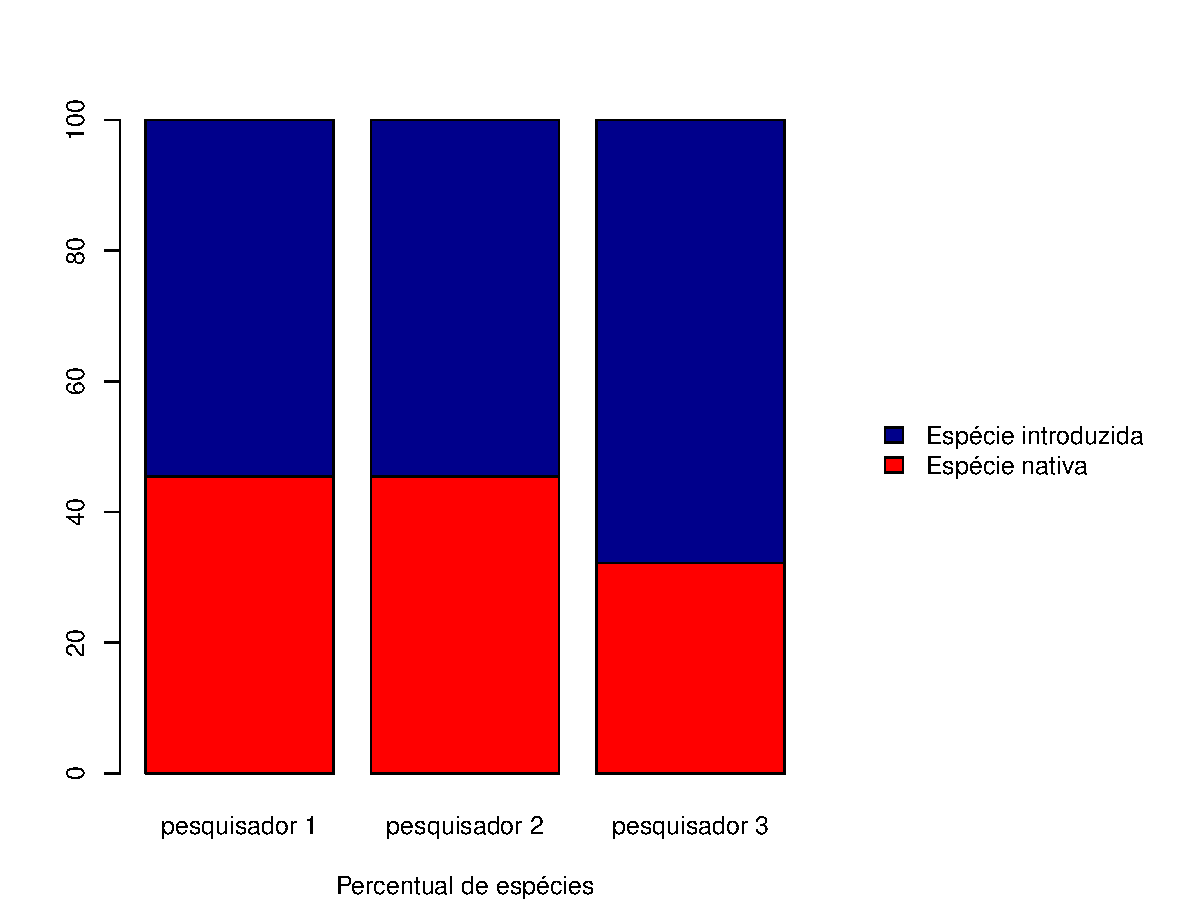
\includegraphics{livroR-1.0_files/figure-latex/bar-tab-1} 

}

\caption{Gráfico de barras sobrepostas indicando o percentual relativo da observação de espécies nativas (cor vermelha) e introduzidas (cor azul), por pesquisador.}\label{fig:bar-tab}
\end{figure}

Como podem ver o nosso gráfico foi realizado. Mas adicionamos uma série de comandos novos. Vamos explica-los passo a passo.

Primeiro contruímos a tabela com os dados em percentuais relativos ao pesquisador e o armazenamos em um objeto chamado tabela.

Posteriormente utilizamos uma função chamada \textcolor{blue}{par()} com o argumento ``mar'' no qual concatenamos 4 valores. Esta função juntamente com esse argumento permite que redimensionemos a janela gráfica. Os quatro valores concatenados referem-se as margens inferior, esquerda, superior e direita, respectivamente.

Nosso último passo é a nossa já conhecida função \textcolor{blue}{barplot()}, onde inserimos como primeiro valor o objeto que contem os dados que queremos graficar \textbf{tabela}, seguido pelo argumento ``col'' que define as cores de acordo com as linhas da tabela, por sua vez definimos se a legenda será plotada com o argumento ``\emph{legend.text}'' e por último indicamos a posição e o formato da legenda por meio do argumento ``\emph{args.lengend}''. Neste último argumento precisamos inserir a função \textcolor{blue}{list()} na qual indicamos a posição da legenda pelo argumento ``x'', o argumento ``bty'' o qual define que a legenda não tera uma caixa desenhada no seu entorno e o argumento ``\emph{inset}'' que define a posição da legenda em relação ao eixo x.

\hypertarget{considerauxe7uxf5es-1}{%
\section{Considerações}\label{considerauxe7uxf5es-1}}

Durante nosso percurso neste capítulo realizamos etapas que consistem na construção dos dados no próprio programa do R e a condução da análise do qui-quadrado para ajuste das frequências e para a independência. A construção dos dados tem como resultado final um objeto similar a planilha de dados que deve ser importada, caso já a tenha preparado, e juntamente com a sumarização dos dados temos as mesmas etapas trabalhadas no capítulo anterior. A partir daí temos a condução da análise estatística pelo qui-quadrado. Um resumo gráfico das etapas pode ser observado aqui (Figura \ref{fig:resumo2}).

\begin{figure}[H]

{\centering 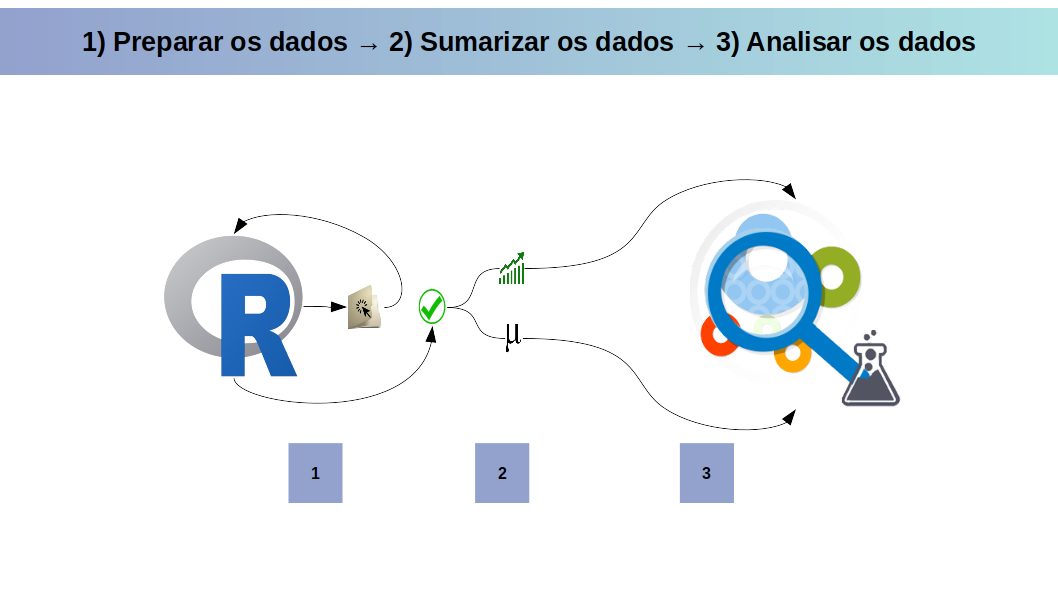
\includegraphics[width=1\linewidth]{/media/wilson/personaldoc/Livro_R/Série estatística passo a passo em excel e R/livroR-1.0/figures print/resumo2} 

}

\caption{Resumo dos passos abordados no capítulo: da preparação dos dados até a análise dos dados.}\label{fig:resumo2}
\end{figure}

\hypertarget{exercuxedcios-2}{%
\section{Exercícios}\label{exercuxedcios-2}}

\begin{enumerate}
\def\labelenumi{\arabic{enumi})}
\item
  Durante um longo período de observação sobre a trafego de carros na praia um pesquisador percebeu que durante a tarde o número de carros circulando era maior que durante a manhã. Ele resolveu tomar nota da quantidade de carros que passava em um determinado trecho da praia, durante vários dias, em ambos os períodos (manhã e tarde) e registrou, no total, os seguintes valores: 550 carros durante a manhã 620 carros durante a tarde. Considerando a observação do pesquisador e os valores por ele tomados, podemos corroborar ou refutar sua observação? Desenvolva a análise do qui-quadrado.
\item
  Ao registrar o número de carros o pesquisador também registrou os dias da semana em que foram feitas as observações e obteve os seguintes valores:
\end{enumerate}

\begin{itemize}
\tightlist
\item
  Manhã de Quarta-feira: 130
\item
  Manhã de Sexta-feira: 420
\item
  Tarde de Quarta-feira: 178
\item
  Tarde de Sexta-feira: 442
  A partir desses registros podemos dizer que o número de carros por período do dia (manhã e tarde) é independente do dia da semana (Quarta-feira e Sexta-feira)?
\end{itemize}

\begin{enumerate}
\def\labelenumi{\arabic{enumi})}
\setcounter{enumi}{2}
\item
  Considerando os dados do exercício anterior. Obtenha a tabela com os dados em percentuais do número de carros por período do dia em relação aos dias da semana.
\item
  Defina erro do tipo 1 e erro do tipo 2. Considerando o exercício 2. Qual dos erros (tipo 1 ou tipo 2) é assumido a um nível de confiança de 95\%?
\item
  Plote um gráfico com a tabela obtida no exercício 3.
\end{enumerate}

\hypertarget{teste-t}{%
\chapter{Teste-t}\label{teste-t}}

Ao iniciarmos nossos estudos geralmente estamos interessados em saber se alguma característica da população que coletamos e analisamos é similar a uma outra população. Podemos abordar essa ideia por diversos caminhos porém vamos iniciar essas análises em R através do teste-t para uma amostra e a discussão sobre hipótese nula, caudalidade e nível de confiança. A partir de então seguiremos para o teste-t com duas amostras e o teste-t pareado.

\hypertarget{teste-t-para-uma-amostra}{%
\section{Teste-t para uma amostra}\label{teste-t-para-uma-amostra}}

Conduzimos esse teste quando objetivamos verificar se a média de uma dada variável é similar a um valor esperado. Ao falarmos de média percebemos que a variável com a qual estamos lidando é do tipo númerica ou inteiro (a diferença entre ambas consiste na presença de casas decimais, na variável númerica), ou seja, mensurável (= quantitativo). Ao compararmos a média de nossa variável a um valor previamente estipulado duas hipóteses são naturalmente construídas, a hipótese nula (H0) e a hipótese alternativa (HA) (Tabela \ref{tab:tab1t}).

\begin{table}

\caption{\label{tab:tab1t}Principais características do teste-t para uma amostra}
\centering
\begin{tabular}[c]{>{\raggedright\arraybackslash}p{10em}>{\raggedright\arraybackslash}p{30em}}
\toprule
Atributos & Características\\
\midrule
\textbf{\cellcolor{gray!6}{Tipo de variável}} & \cellcolor{gray!6}{Quantitativa}\\
\textbf{Quantidade de variáveis} & 1\\
\textbf{\cellcolor{gray!6}{Hipótese nula}} & \cellcolor{gray!6}{A média da variável é similar ao valor previamente estipulado}\\
\textbf{Fórmula} & $$t=\frac{(\overline{X}-\mu)}{(s/sqrt(N))}$$ Onde, $\overline{X}$: média da amostra, $\mu$: média teórica esperada, s: desvio padrão da amostra e N: tamanho da amostra.\\
\textbf{\cellcolor{gray!6}{Observação}} & \cellcolor{gray!6}{Não há a necessidade de post-hoc nem expressa-la graficamente}\\
\bottomrule
\end{tabular}
\end{table}

Caso você ainda não tenha seus dados, vamos verificar como conduzir o teste-t por meio de exemplos utilizando valores fictícios.

Imagine o seguinte exemplo: 100 camarões foram coletados em um estuário. Suas medidas em relação ao tamanho foram tomadas e deseja-se saber se o seu tamanho médio é similar ou não ao tamanho médio (25,80mm) da mesma espécie, observada em outro estuário.

A partir do exemplo acima podemos definir nossas hipóteses, onde.

\begin{itemize}
\tightlist
\item
  H0: média observada é igual à média esperada;
\item
  HA: média observada é diferente da média esperada;
\end{itemize}

Vamos começar gerando os dados relativos ao tamanho observado dos camarões que coletamos.

Para isso vamos utilizar a função \textcolor{blue}{set.seed()} que define os números aleatórios que serão gerados. Dessa forma, quando aplicado essa função associada a um número comum, no caso ``1234'', os números aleatórios que você irá gerar para o objeto \textbf{tamanho.camarao}, por exemplo, serão os mesmos dos apresentados aqui.

A nossa segunda linha de comando utilizará a função \textcolor{blue}{rnorm()} o qual gera números aleatórios considerando uma distribuição normal e soma esses valores gerados a uma distribuição uniforme gerada pela função \textcolor{blue}{runif()}. A estas funções adicionamos argumentos que definem a quantidade de números gerados (argumento ``n''), o valor mínimo que pode ser gerado (argumento ``min'') e o valor máximo que pode ser gerado (argumento ``max''). E guardamos o resultado obtido em um objeto chamado \textbf{tamanho.camarao}. Relembre que o nome do objeto não deve apresentar espaços ou acentos, que pode gerar problemas e/ou dificuldades na condução das análises.

\begin{Shaded}
\begin{Highlighting}[]
\KeywordTok{set.seed}\NormalTok{(}\DecValTok{1234}\NormalTok{)}
\NormalTok{tamanho.camarao <-}\StringTok{ }\KeywordTok{rnorm}\NormalTok{(}\DataTypeTok{n =} \DecValTok{100}\NormalTok{) }\OperatorTok{+}\StringTok{ }\KeywordTok{runif}\NormalTok{(}\DataTypeTok{n =} \DecValTok{100}\NormalTok{, }\DataTypeTok{min =} \DecValTok{17}\NormalTok{, }\DataTypeTok{max =} \DecValTok{33}\NormalTok{)}
\end{Highlighting}
\end{Shaded}

Vamos verificar o resultado. Basta digitarmos o nome do objeto.

\begin{Shaded}
\begin{Highlighting}[]
\NormalTok{tamanho.camarao}
\end{Highlighting}
\end{Shaded}

\begin{verbatim}
##   [1] 26.36501 25.73118 23.16434 26.93999 25.85006 29.22289 21.34791 22.92014
##   [9] 19.70599 31.88009 25.58378 20.48762 19.18464 29.19344 27.02799 31.80449
##  [17] 26.70808 27.30077 23.83039 33.02083 23.89138 17.01159 20.68980 22.81711
##  [25] 18.44307 23.54454 30.40893 21.37080 25.12759 23.97507 30.85514 25.59575
##  [33] 17.99771 29.42112 24.44470 19.22824 26.81323 20.57450 24.53800 32.36946
##  [41] 25.23524 19.84181 19.61879 27.74526 31.68906 23.66401 28.26906 24.93702
##  [49] 31.93121 29.25393 23.70445 25.96390 20.11329 20.45772 17.87934 26.57236
##  [57] 22.84551 16.27916 28.03817 24.16301 31.17074 20.02190 26.56155 20.62508
##  [65] 18.92214 20.38837 27.83197 18.62320 19.12094 29.29845 22.72270 28.68786
##  [73] 22.64878 30.43969 19.48136 24.94834 28.74896 24.99252 21.52521 22.19714
##  [81] 22.72903 23.69804 30.32393 29.37573 29.65554 22.18997 24.85922 21.19787
##  [89] 27.94906 28.93757 27.42930 23.87127 33.93523 21.89126 26.24338 29.48277
##  [97] 26.96407 19.72505 28.14750 24.06552
\end{verbatim}

Vamos observar as métricas e gráficos, conforme já fizemos nos capítulos anteriores, mas relativos ao objeto criado.

\begin{Shaded}
\begin{Highlighting}[]
\KeywordTok{mean}\NormalTok{(tamanho.camarao)}
\end{Highlighting}
\end{Shaded}

\begin{verbatim}
## [1] 24.86218
\end{verbatim}

\begin{Shaded}
\begin{Highlighting}[]
\KeywordTok{min}\NormalTok{(tamanho.camarao)}
\end{Highlighting}
\end{Shaded}

\begin{verbatim}
## [1] 16.27916
\end{verbatim}

\begin{Shaded}
\begin{Highlighting}[]
\KeywordTok{max}\NormalTok{(tamanho.camarao)}
\end{Highlighting}
\end{Shaded}

\begin{verbatim}
## [1] 33.93523
\end{verbatim}

\begin{Shaded}
\begin{Highlighting}[]
\KeywordTok{length}\NormalTok{(tamanho.camarao)}
\end{Highlighting}
\end{Shaded}

\begin{verbatim}
## [1] 100
\end{verbatim}

\begin{Shaded}
\begin{Highlighting}[]
\KeywordTok{hist}\NormalTok{(tamanho.camarao)}
\end{Highlighting}
\end{Shaded}

\begin{figure}[H]

{\centering 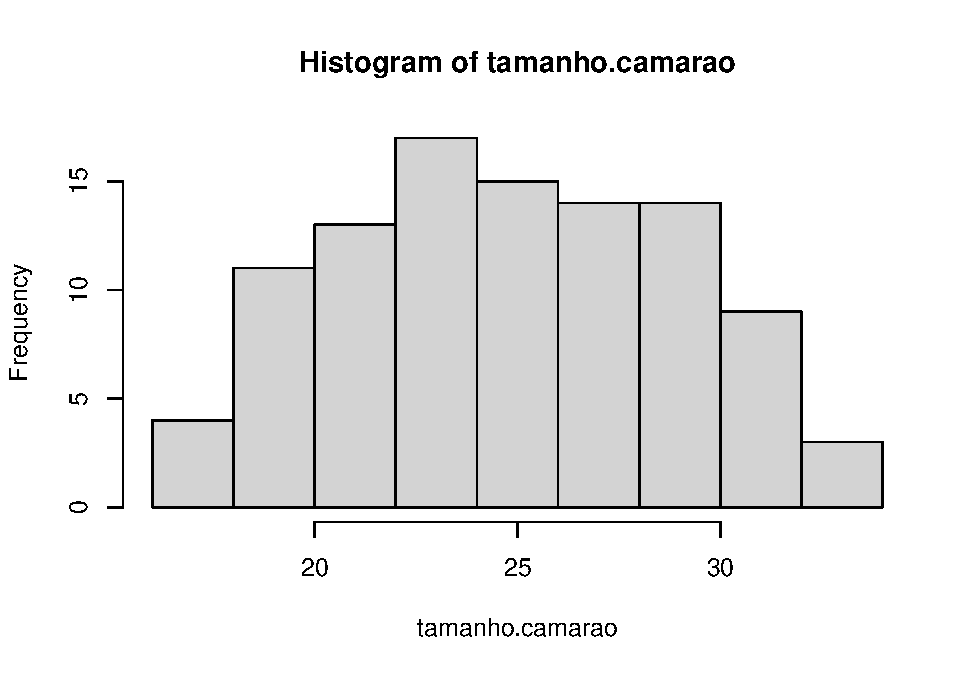
\includegraphics[width=0.7\linewidth]{livroR-1.0_files/figure-latex/hist-tam-cam-1} 

}

\caption{Histograma dos valores do objeto relativo ao tamanho dos camarões}\label{fig:hist-tam-cam}
\end{figure}

Como podemos ver os valores mínimo e máximo são similares ao que definimos e o número de elementos é o mesmo. Graficamente podemos ver que a distribuição é normal, pois como vimos utilizamos uma função que cria uma distribuição normal com limites definidos pela função \textcolor{blue}{runif()}. Além disso vemos que há uma maior frequência dos valores em torno de 25 (Figura \ref{fig:hist-tam-cam}).

Vamos verificar se esse valor que geramos (obtivemos de tamanho do camarão) são similares ao observado em outra localidade, por meio do teste-t para uma amostra. Para isso imaginemos que o valor médio esperado para o tamanho desta espécie de camarão em outra localidade é de 25,80mm. Para isso iremos criar o objeto \textbf{esperado} que contem esse valor.

\begin{Shaded}
\begin{Highlighting}[]
\NormalTok{esperado =}\StringTok{ }\FloatTok{25.80}
\end{Highlighting}
\end{Shaded}

Agora vamos, por meio da função \textcolor{blue}{t.test()} realizar o teste-t para verificar se os nossos dados tem média similar ao esperado.

\begin{Shaded}
\begin{Highlighting}[]
\KeywordTok{t.test}\NormalTok{(}\DataTypeTok{x =}\NormalTok{ tamanho.camarao, }\DataTypeTok{mu =}\NormalTok{ esperado)}
\end{Highlighting}
\end{Shaded}

\begin{verbatim}
## 
##  One Sample t-test
## 
## data:  tamanho.camarao
## t = -2.2432, df = 99, p-value = 0.02711
## alternative hypothesis: true mean is not equal to 25.8
## 95 percent confidence interval:
##  24.03263 25.69173
## sample estimates:
## mean of x 
##  24.86218
\end{verbatim}

O primeiro argumento da função \textcolor{blue}{t.test()}: ``x'' refere-se ao nosso objeto que contem os dados referentes ao tamanho que coletamos (\textbf{tamanho.camarao}) e o segundo argumento ``mu'' refere-se ao objeto que contem a média do tamanho obtido em outro estuário (\textbf{esperado}).

Conforme podemos visualizar no resultado temos 9 linhas. A primeira linha nos diz qual teste está sendo conduzido, neste caso é (\emph{One Sample t-test} ou teste-t para uma amostra), a segunda linha nos retorna o conjunto de dados que utilizamos, a terceira linha nos retorna o valor do teste-t (\emph{t} = -2,2432) o grau de liberdade (\emph{df} = 99) e o valor de probabilidade associado ao teste (\emph{p-value} = 0,02711), a quarta linha nos retorna qual é nossa hipótese alternativa, caso a aceitemos (a qual nos diz que: a média dos nossos dados não é igual à 25,8), a quinta e sexta linhas nos fornece o intervalo de confiança de 95\% dos nossos dados (24,03263 e 25,69173) e da sétima a nona linha refere-se a informação relativa a média dos nossos dados (24,86218).

Em resumo, podemos inferir que a média dos nossos dados é diferente do valor esperado pois o \emph{p-value} foi menor que 0,05. Detalhadamente podemos dizer que: a média do tamanho dos camarões que coletamos (24,86 mm) é estatisticamente menor do que a média presente no outro estuário (25,80 mm) a um nível de confiança de 95\%, portanto rejeitamos H0.

Ok, verificamos e entendemos como conduzir a análise. Mas há um conceito estatístico importante na análise do teste-t, a caudalidade. No exemplo anterior nós trabalhamos com as hipóteses de que a média de um conjunto de dados é igual (H0) ou diferente (HA) da média esperada. O que implica em dizer que a média que observamos pode ser maior ou menor do que o esperado. Contudo em algumas instâncias podemos querer verificar se a média do nosso conjunto de dados é maior ou igual ou menor ou igual a média esperada e não diferente. Desta diferença na construção da hipótese que emerge o conceito da caudalidade. No exemplo anterior foi testado a hipótese bicaudal que é tido como padrão (\emph{default}) na função do R que executamos.

A diferença do teste-t bicaudal para o unicaudal depende da pergunta e hipótese levantada previamente. Então antes de realizar este teste mantenha-se atento ao que se deseja testar.

Vejamos o seguinte exemplo: Em um costão rochoso foi observado ao longo do ``dia 1'' 100 estrelas do mar em diferentes alturas, em relação a baixamar. Essas alturas foram mensuradas (valores serão construídos abaixo no objeto denominado \textbf{estrela}). Sabe-se que no dia anterior ``dia 0'' a altura média das estrelas no mesmo costão foi de 0,90m. Sabe-se também que o ``dia 0'' foi mais frio e que dias mais frios implicam em maiores alturas.

Neste exemplo estamos interessado em saber se a altura das estrelas do mar no ``dia 1'' é menor que a do ``dia 0'', visto que o ``dia 1'' é mais quente.

A partir dessas informações podemos construir as seguintes hipóteses:

\begin{itemize}
\tightlist
\item
  H0: A média da altura das estrelas do mar no dia 1 é maior ou igual ao dia 0;
\item
  HA: A média da altura das estrelas do mar no dia 1 é menor que a do dia 0;
\end{itemize}

Matematicamente podemos escrever as hipóteses da seguinte forma:

\begin{itemize}
\tightlist
\item
  H0: \(\mu_{dia.1} \geq \mu_{dia.0}\)
\item
  HA: \(\mu_{dia.1} < \mu_{dia.0}\)
\end{itemize}

De maneira similar ao exemplo anterior vamos gerar nosso conjunto de dados que contêm os valores de altura das estrelas do mar no costão rochoso, a diferença é que iremos inserir o argumento ``sd'' na função \textcolor{blue}{rnorm()} que corresponde ao desvio padrão (de 0,02) dos dados normais que estamos gerando e guardar esse resultado no objeto \textbf{estrelas}.

\begin{Shaded}
\begin{Highlighting}[]
\KeywordTok{set.seed}\NormalTok{(}\DecValTok{1234}\NormalTok{)}
\NormalTok{estrelas <-}\StringTok{ }\KeywordTok{rnorm}\NormalTok{(}\DataTypeTok{n =} \DecValTok{100}\NormalTok{, }\DataTypeTok{sd =} \FloatTok{0.02}\NormalTok{) }\OperatorTok{+}\StringTok{ }\KeywordTok{runif}\NormalTok{(}\DataTypeTok{n =} \DecValTok{100}\NormalTok{, }\DataTypeTok{min =} \FloatTok{0.4}\NormalTok{, }\DataTypeTok{max =} \FloatTok{1.3}\NormalTok{)}
\end{Highlighting}
\end{Shaded}

Conforme também fizemos anteriormente calcularemos algumas métricas para entender os dados e um histograma básico (Figura \ref{fig:estrelas-hist}) para visualizar a forma dos dados que representam a altura que as estrelas se encontram no ambiente.

\begin{Shaded}
\begin{Highlighting}[]
\KeywordTok{mean}\NormalTok{(estrelas)}
\end{Highlighting}
\end{Shaded}

\begin{verbatim}
## [1] 0.8479302
\end{verbatim}

\begin{Shaded}
\begin{Highlighting}[]
\KeywordTok{min}\NormalTok{(estrelas)}
\end{Highlighting}
\end{Shaded}

\begin{verbatim}
## [1] 0.387487
\end{verbatim}

\begin{Shaded}
\begin{Highlighting}[]
\KeywordTok{max}\NormalTok{(estrelas)}
\end{Highlighting}
\end{Shaded}

\begin{verbatim}
## [1] 1.290766
\end{verbatim}

\begin{Shaded}
\begin{Highlighting}[]
\KeywordTok{length}\NormalTok{(estrelas)}
\end{Highlighting}
\end{Shaded}

\begin{verbatim}
## [1] 100
\end{verbatim}

\begin{Shaded}
\begin{Highlighting}[]
\KeywordTok{hist}\NormalTok{(estrelas)}
\end{Highlighting}
\end{Shaded}

\begin{figure}[H]

{\centering 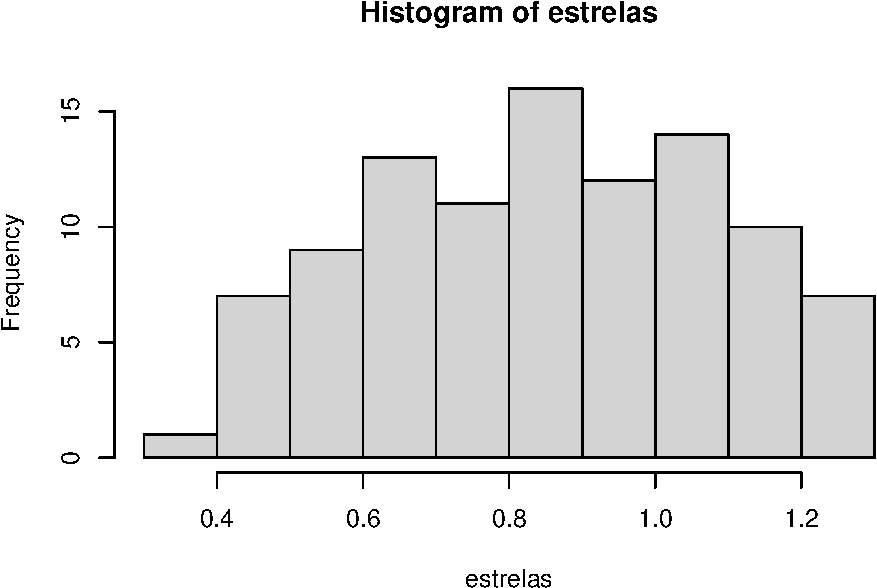
\includegraphics[width=0.7\linewidth]{livroR-1.0_files/figure-latex/estrelas-hist-1} 

}

\caption{Histograma dos valores relativos a altura das estrelas do mar no costão rochoso}\label{fig:estrelas-hist}
\end{figure}

Agora vamos criar o objeto \textbf{dia.0} que contêm o valor referente a altura das estrelas no dia 0.

\begin{Shaded}
\begin{Highlighting}[]
\NormalTok{dia}\FloatTok{.0}\NormalTok{ =}\StringTok{ }\FloatTok{0.90}
\end{Highlighting}
\end{Shaded}

Agora o teste-t onde avaliaremos se a média da altura das estrelas do mar que obtivemos para o ``dia 1'' são maiores ou iguais ao ``dia 0'', utilizando o argumento ``\emph{alternative}'' e definido-o como \emph{less}. Este argumento pode ser definido de 3 formas: \emph{two-sided} que é o padrão (\emph{default}), \emph{greater} ou \emph{less}. O argumento ``\emph{alternative}'' seguirá o sinal da hipótese alternativa (HA) que foi construída para o teste.

\begin{Shaded}
\begin{Highlighting}[]
\KeywordTok{t.test}\NormalTok{(}\DataTypeTok{x =}\NormalTok{ estrelas, }\DataTypeTok{mu =}\NormalTok{ dia}\FloatTok{.0}\NormalTok{, }\DataTypeTok{alternative =} \StringTok{"less"}\NormalTok{)}
\end{Highlighting}
\end{Shaded}

\begin{verbatim}
## 
##  One Sample t-test
## 
## data:  estrelas
## t = -2.2073, df = 99, p-value = 0.0148
## alternative hypothesis: true mean is less than 0.9
## 95 percent confidence interval:
##       -Inf 0.8870986
## sample estimates:
## mean of x 
## 0.8479302
\end{verbatim}

Com isso podemos avaliar o resultado que é similar ao que vimos anteriormente com poucas mudanças. A primeira linha (\emph{One Sample t-test}) informa sobre o teste realizado. A segunda linha indica o nome do conjunto de dados que inserimos. A terceira linha nos dá o valor do teste-t (\emph{t} = -2,2073), do grau de liberdade (\emph{df} = 99) e da probabilidade associada ao teste (\emph{p-value} = 0.0148). A quarta linha indica a hipótese alternativa, caso seja aceita (o que é o caso), que é verdade que a média da altura das estrelas do mar do ``dia 1'' é menor que 0,90m. A quinta e sexta linha indicam o intervalo de confiança de 95\% dos nossos dados (-Inf e 0,8870986). A sétima, oitava e nona linha referem-se a média do ``dia 1''.

Como podemos notar pelo \emph{p-value} rejeitamos nossa hipótese nula (H0). Portanto a média na altura das estrelas do mar do ``dia 1'' (aproximadamente 0,85m) é menor que a do dia ``0'' (0,90m).

Outro conceito importante de qualquer teste inferencial é o nível de confiança\footnote{Consiste na subtração do nível de significância (alfa) de 1. Ou seja: nível de confiança = 1 - alfa.}. Até o presente momento consideramos o nível de confiança de 95\%. Se quisermos altera-lo no teste-t devemos adicionar o argumento ``conf.level'' em proporção (valores entre 0 e 1). A sua alteração implica na alteração do nível de significância e consequentemente na zona de rejeição da hipótese nula. Se aumentarmos o seu valor fica mais difícil rejeitarmos a hipótese nula e se diminuirmos o seu valor fica mais fácil rejeitar a hipótese nula. Vejamos outro exemplo.

Um pesquisador avaliou o tamanho de cracas incrustadas no casco de uma embarcação. Objetivando saber se o tamanho médio de cracas difere do teórico esperado (13,5 mm) um teste-t bicaudal foi aplicado a um nível de confiança de 95\% e 99\%.

Vamos descrever as hipóteses e realizar a análise para ambos os níveis de confiança.

Neste caso temos as seguintes hipóteses:

\begin{itemize}
\tightlist
\item
  H0: O tamanho médio observado é similar ao teórico
\item
  HA: O tamanho médio observado difere do teórico
\end{itemize}

Conforme já realizado anteriormente vamos gerar os dados iguais aos gerados aqui por meio das funções \textcolor{blue}{set.seed()}, \textcolor{blue}{rnorm()} e \textcolor{blue}{runif()}, guardando o seu resultado em um objeto chamado \textbf{cracas}e explora-los com algumas métricas estatśticas e gráficas de maneira similar ao que fizemos no exemplo anterior.

\begin{Shaded}
\begin{Highlighting}[]
\KeywordTok{set.seed}\NormalTok{(}\DecValTok{1234}\NormalTok{)}
\NormalTok{cracas <-}\StringTok{ }\KeywordTok{rnorm}\NormalTok{(}\DataTypeTok{n =} \DecValTok{100}\NormalTok{, }\DataTypeTok{sd =} \FloatTok{1.9}\NormalTok{) }\OperatorTok{+}\StringTok{ }\KeywordTok{runif}\NormalTok{(}\DataTypeTok{n =} \DecValTok{100}\NormalTok{, }\DataTypeTok{min =} \DecValTok{5}\NormalTok{, }\DataTypeTok{max =} \DecValTok{25}\NormalTok{)}
\KeywordTok{mean}\NormalTok{(cracas)}
\end{Highlighting}
\end{Shaded}

\begin{verbatim}
## [1] 14.72583
\end{verbatim}

\begin{Shaded}
\begin{Highlighting}[]
\KeywordTok{min}\NormalTok{(cracas)}
\end{Highlighting}
\end{Shaded}

\begin{verbatim}
## [1] 3.596275
\end{verbatim}

\begin{Shaded}
\begin{Highlighting}[]
\KeywordTok{max}\NormalTok{(cracas)}
\end{Highlighting}
\end{Shaded}

\begin{verbatim}
## [1] 27.27792
\end{verbatim}

\begin{Shaded}
\begin{Highlighting}[]
\KeywordTok{length}\NormalTok{(cracas)}
\end{Highlighting}
\end{Shaded}

\begin{verbatim}
## [1] 100
\end{verbatim}

\begin{Shaded}
\begin{Highlighting}[]
\KeywordTok{hist}\NormalTok{(cracas)}
\end{Highlighting}
\end{Shaded}

\begin{figure}[H]

{\centering 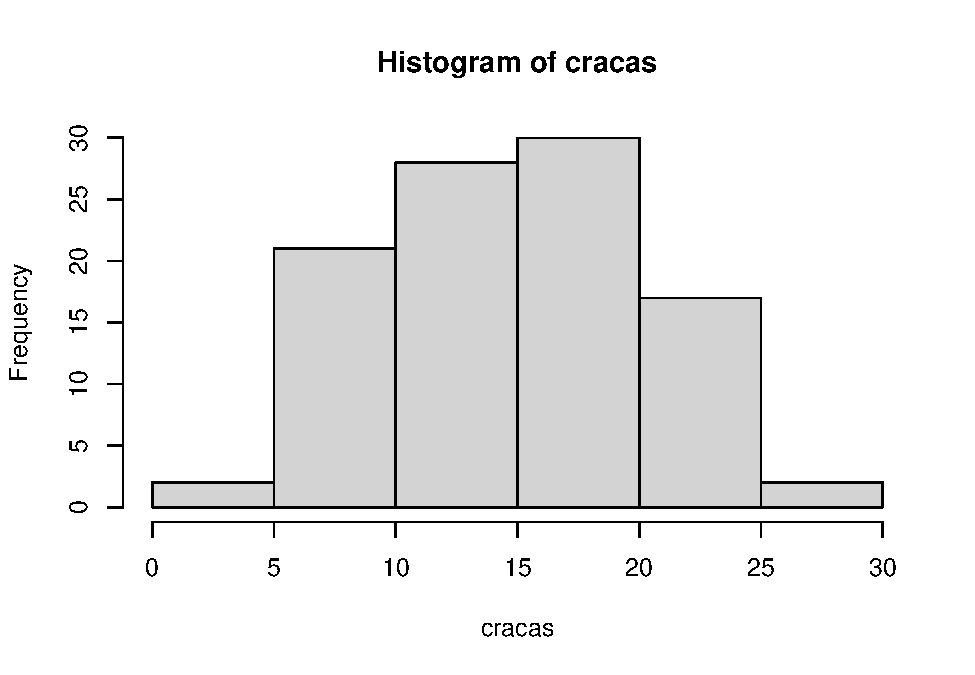
\includegraphics[width=0.7\linewidth]{livroR-1.0_files/figure-latex/craca-hist-1} 

}

\caption{Histograma dos valores relativos ao tambanho das cracas incrustantes}\label{fig:craca-hist}
\end{figure}

Agora que visualizamos as métricas e graficamos os dados (Figura \ref{fig:craca-hist}), sigamos construindo o objeto que guarda o valor teórico (13,5mm) e com a condução da análise.

\begin{Shaded}
\begin{Highlighting}[]
\NormalTok{teorico <-}\StringTok{ }\FloatTok{13.5}
\KeywordTok{t.test}\NormalTok{(}\DataTypeTok{x =}\NormalTok{ cracas, }\DataTypeTok{mu =}\NormalTok{ teorico, }\DataTypeTok{conf.level =} \FloatTok{0.95}\NormalTok{)}
\end{Highlighting}
\end{Shaded}

\begin{verbatim}
## 
##  One Sample t-test
## 
## data:  cracas
## t = 2.3113, df = 99, p-value = 0.02289
## alternative hypothesis: true mean is not equal to 13.5
## 95 percent confidence interval:
##  13.67349 15.77817
## sample estimates:
## mean of x 
##  14.72583
\end{verbatim}

\begin{Shaded}
\begin{Highlighting}[]
\KeywordTok{t.test}\NormalTok{(}\DataTypeTok{x =}\NormalTok{ cracas, }\DataTypeTok{mu =}\NormalTok{ teorico, }\DataTypeTok{conf.level =} \FloatTok{0.99}\NormalTok{)}
\end{Highlighting}
\end{Shaded}

\begin{verbatim}
## 
##  One Sample t-test
## 
## data:  cracas
## t = 2.3113, df = 99, p-value = 0.02289
## alternative hypothesis: true mean is not equal to 13.5
## 99 percent confidence interval:
##  13.33290 16.11876
## sample estimates:
## mean of x 
##  14.72583
\end{verbatim}

Como podem ver ambos os resultados (com diferentes níveis de confiança) retornam o mesmo valor do teste-t e do \emph{p-value}. E neste ponto precisamos ir com calma para evitar erro de interpretação do resultado e entender estatisticamente o que está acontencendo.

Quando representamos o nível de confiança (representado pelo argumento ``conf.level'') por um valor probabilístico de 0,95 ou 0,99 estamos dizendo que o nível de significância é 0,05 e 0,01, respectivamente. Quando olhamos para o resultado do \emph{p-value}, temos que levar em consideração o nível de significância.

Vejamos o nosso resultado.

No primeiro caso (``\emph{conf.level} = 0.95'') temos \emph{p-value} = 0,02289, como este valor é menor que 0,05 (nosso nível de significância), isso quer dizer que a média teórica está fora do intervalo de confiança dos dados, portanto rejeitamos a hipótese nula.

No segundo caso (``conf.level = 0.99'') temos o mesmo \emph{p-value} (0,02289), contudo este valor é maior que nosso nível de significância (0,01), isso quer dizer que nossa média teórica está dentro do intervalo de confiança, portanto aceitamos a hipótese nula de que a média observada é similar a média teórica.

\textcolor{red}{OBS: Em um primeiro momento pode parecer confuso, portanto releia o exemplo acima, assim como outras literaturas.}

O nível de significância a aplicar nos seus dados depende das informações que possui sobre o organismo ou o ambiente que está estudando. Apesar da regra-de-bolso dizer 0,05 e por padrão o R definir esse nível de significância é necessário entender o que ele representa para seus dados e qual a implicação para sua hipótese e as medidas que serão tomadas. Uma dica importante é: reporte sempre o intervalo de confiança, indique o nível de significância que foi aplicado e no seu texto deixe claro o porquê de sua escolha, principalmente se for diferente do que é definido como padrão.

\textbf{BÔNUS:}

Embora não seja comum, podemos plotar um gráfico que represente o nosso resultado estatístico como uma curva de densidade no qual é representado o valor do teste-t, o grau de liberdade e o valor de probabilidade associado. Para isso vamos usar um pacote o qual precisa ser instalado chamado \textcolor{brown}{webr} e precisamos carrega-lo usando a função \textcolor{blue}{library()}. Após isso é só inserir a função que desenvolve o teste-t dentro da função \textcolor{blue}{plot()}. Veja o resultado para ambos os níveis de confiança estabelecidos previamente.

\textcolor{red}{OBS: Uma vez instalado o pacote não precisa instala-lo novamente apenas carrega-lo se estiver iniciando o R pela primeira vez.}

\begin{Shaded}
\begin{Highlighting}[]
\KeywordTok{install.packages}\NormalTok{(}\StringTok{"webr"}\NormalTok{)}
\KeywordTok{library}\NormalTok{(webr)}
\end{Highlighting}
\end{Shaded}

Após instalar e carregar o pacote devemos inserir o teste-t dentro da função \textcolor{blue}{plot()}. Veja os dois exemplos abaixo.

\begin{Shaded}
\begin{Highlighting}[]
\KeywordTok{plot}\NormalTok{(}\KeywordTok{t.test}\NormalTok{(}\DataTypeTok{x =}\NormalTok{ cracas, }\DataTypeTok{mu =}\NormalTok{ teorico, }\DataTypeTok{conf.level =} \FloatTok{0.95}\NormalTok{))}
\end{Highlighting}
\end{Shaded}

\begin{figure}[H]

{\centering 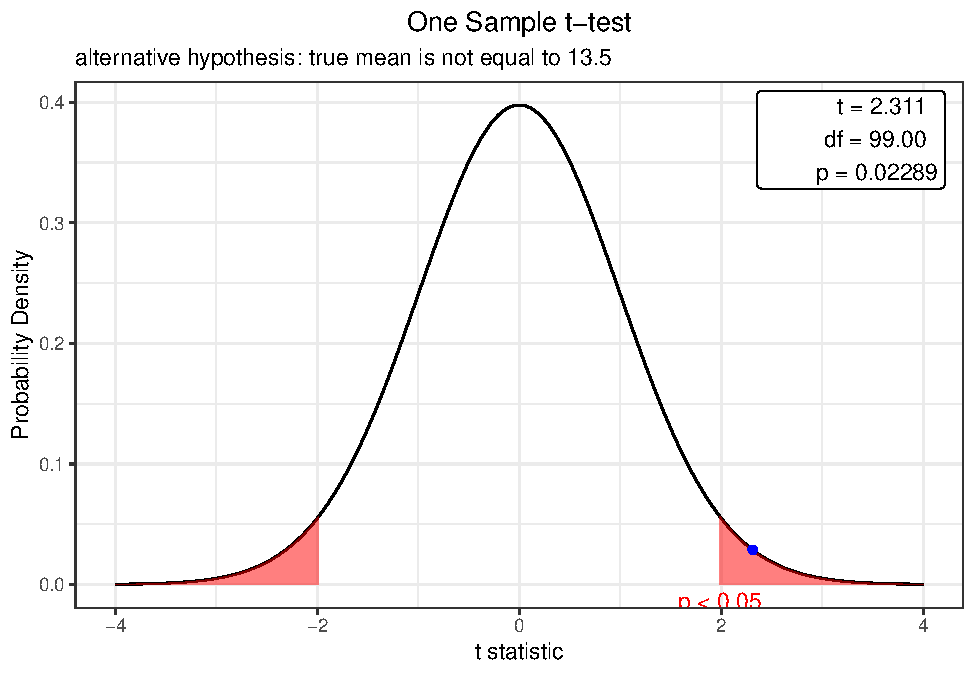
\includegraphics[width=0.7\linewidth]{livroR-1.0_files/figure-latex/cracas-dens-95-1} 

}

\caption{Curva de densidade representando o valor do teste-t bicaudal para o tamanho das cracas em relação a média teórica a um intervalo de confiança de 95\%. O ponto azul indica o valor do teste.}\label{fig:cracas-dens-95}
\end{figure}

\begin{Shaded}
\begin{Highlighting}[]
\KeywordTok{plot}\NormalTok{(}\KeywordTok{t.test}\NormalTok{(}\DataTypeTok{x =}\NormalTok{ cracas, }\DataTypeTok{mu =}\NormalTok{ teorico, }\DataTypeTok{conf.level =} \FloatTok{0.99}\NormalTok{))}
\end{Highlighting}
\end{Shaded}

\begin{figure}[H]

{\centering 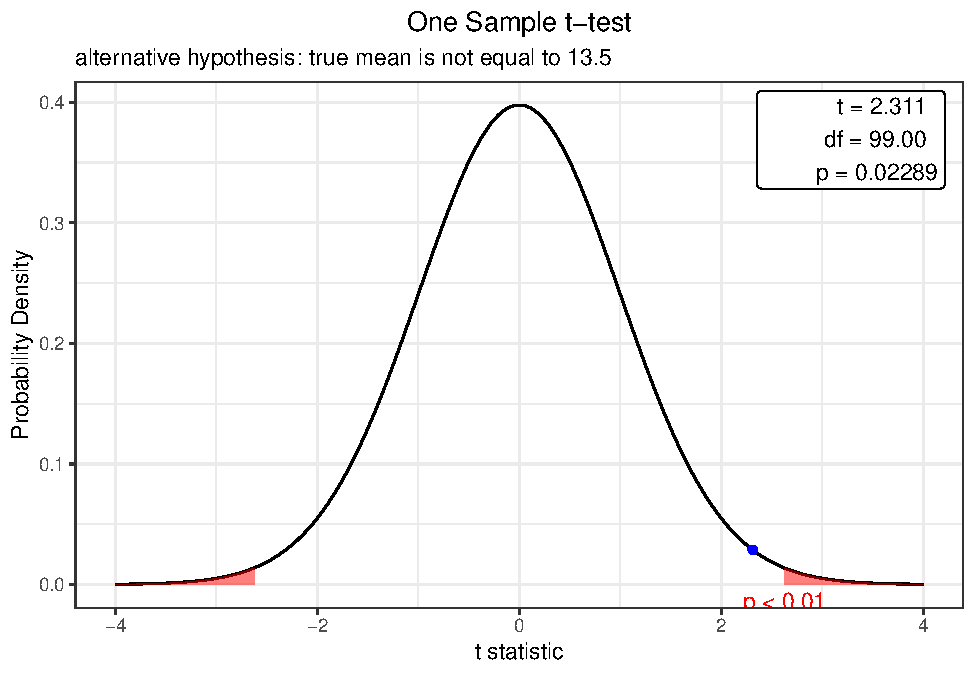
\includegraphics[width=0.7\linewidth]{livroR-1.0_files/figure-latex/cracas-dens-99-1} 

}

\caption{Curva de densidade representando o valor do teste-t bicaudal para o tamanho das cracas em relação a média teórica a um intervalo de confiança de 99\%. O ponto azul indica o valor do teste.}\label{fig:cracas-dens-99}
\end{figure}

Verifique que esses plots nos fornecem as curvas do teste-t os intervalos de confiança de 95\% (Figura \ref{fig:cracas-dens-95}) e 99\% (Figura \ref{fig:cracas-dens-99}), demarca os limites inferior e superior de vermelho e marca como ponto azul na curva de densidade o valor do teste-t associado. Como esse valor está dentro da região demarcada no intervalo de confiança de 95\%, neste caso rejeitamos a hipótese nula e como no intervalo de confiança de 99\% o ponto azul está fora da região demarcada aceitamos a hipótese nula.

\hypertarget{teste-t-para-duas-amostras}{%
\section{Teste-t para duas amostras}\label{teste-t-para-duas-amostras}}

Conduzimos esse teste quando objetivamos comparar se a média de dois grupos são similares (Tabela \ref{tab:tab2t}).

\begin{table}

\caption{\label{tab:tab2t}Principais características do teste-t para duas amostras}
\centering
\begin{tabular}[c]{>{\raggedright\arraybackslash}p{10em}>{\raggedright\arraybackslash}p{30em}}
\toprule
Atributos & Características\\
\midrule
\textbf{\cellcolor{gray!6}{Tipo de variável}} & \cellcolor{gray!6}{Quantitativa e categórica}\\
\textbf{Quantidade de variáveis} & 2 (1 de cada tipo obrigatoriamente)\\
\textbf{\cellcolor{gray!6}{Hipótese nula}} & \cellcolor{gray!6}{A diferença na média da variável quantitativa dos grupos é igual a 0.}\\
\textbf{Fórmula} & $$t=\frac{\overline{X}_1-\overline{X}_2}{s_{\overline{X}_1-\overline{X}_2}}$$, onde, $\overline{X}_1$: média do grupo 1, $\overline{X}_2$: média do grupo 2, s: erro padrão da diferença entre os dois grupos.\\
\textbf{\cellcolor{gray!6}{Observação}} & \cellcolor{gray!6}{Não há a necessidade de post-hoc nem expressa-la graficamente.}\\
\bottomrule
\end{tabular}
\end{table}

Partindo desse objetivo as hipóteses nula e alternativa desse teste podem ser escritas da seguinte forma:

\begin{itemize}
\tightlist
\item
  H0: A diferença na média da variável quantitativa dos grupos é igual a 0;
\item
  HA: A diferença na média da variável quantitativa dos grupos é diferente de 0;
\end{itemize}

Outra forma de apresentarmos as hipóteses relativa a este teste é:

\begin{itemize}
\tightlist
\item
  H0: A média da variável quantitativa é igual entre grupos;
\item
  HA: A média da variável quantitativa é diferente entre grupos;
\end{itemize}

Outra forma de escrevermos a hipótese é em relação a caudalidade do teste e, se unicaudal, pode ser escrita da seguinte forma:

\begin{itemize}
\tightlist
\item
  H0: A média da variável quantitativa é maior ou igual (ou menor ou igual) entre grupos;
\item
  HA: A média da variável quantitativa é menor (ou maior) entre grupos;
\end{itemize}

A partir desse teste, alguns pressupostos estatísticos precisam ser avaliados e portanto algumas análises precisam ser realizadas antes da interpretação do resultado do teste-t. Pressupostos como normalidade (ambos os grupos devem provir de uma população com distribuição normal) e homocedasticidade (A variância entre os dois grupos devem ser iguais). Demonstraremos a frente como realizar alguns desses testes. Mas, primeiro vamos gerar os dados a serem trabalhados para esta etapa. Execute o código abaixo e você irá visualizar no \emph{environment} do seu RStudio um objeto chamado \textbf{gastropode} que corresponde a um \emph{data frame} com o conjunto de dados que iremos trabalhar.

\textcolor{red}{OBS: Neste momento não entraremos em detalhes sobre os comandos aplicados para construção dos dados.}

\begin{Shaded}
\begin{Highlighting}[]
\NormalTok{grupos <-}\StringTok{ }\KeywordTok{c}\NormalTok{(}\KeywordTok{rep}\NormalTok{(}\DataTypeTok{x =} \StringTok{"Alimento A"}\NormalTok{, }\DecValTok{50}\NormalTok{), }\KeywordTok{rep}\NormalTok{(}\DataTypeTok{x =} \StringTok{"Alimento B"}\NormalTok{, }\DecValTok{50}\NormalTok{))}
\KeywordTok{set.seed}\NormalTok{(}\DecValTok{123}\NormalTok{)}
\NormalTok{alimento.A <-}\StringTok{ }\KeywordTok{rnorm}\NormalTok{(}\DataTypeTok{n =} \DecValTok{50}\NormalTok{, }\DataTypeTok{mean =} \FloatTok{0.7}\NormalTok{, }\DataTypeTok{sd =} \FloatTok{0.2}\NormalTok{)}
\KeywordTok{set.seed}\NormalTok{(}\DecValTok{4321}\NormalTok{)}
\NormalTok{alimento.B <-}\StringTok{ }\KeywordTok{rnorm}\NormalTok{(}\DataTypeTok{n =} \DecValTok{50}\NormalTok{, }\DataTypeTok{mean =} \FloatTok{0.2}\NormalTok{, }\DataTypeTok{sd =} \FloatTok{0.2}\NormalTok{)}
\NormalTok{Alimento <-}\StringTok{ }\KeywordTok{c}\NormalTok{(alimento.A, alimento.B)}
\NormalTok{gastropode <-}\StringTok{ }\KeywordTok{as.data.frame}\NormalTok{(}\KeywordTok{cbind}\NormalTok{(grupos, }\KeywordTok{round}\NormalTok{(Alimento, }\DecValTok{3}\NormalTok{)))}
\KeywordTok{colnames}\NormalTok{(gastropode) <-}\StringTok{ }\KeywordTok{c}\NormalTok{(}\StringTok{"Alimento"}\NormalTok{, }\StringTok{"Peso"}\NormalTok{)}
\KeywordTok{rm}\NormalTok{(}\DataTypeTok{list =} \StringTok{"grupos"}\NormalTok{, }\StringTok{"alimento.A"}\NormalTok{, }\StringTok{"alimento.B"}\NormalTok{, }\StringTok{"Alimento"}\NormalTok{)}
\end{Highlighting}
\end{Shaded}

Vamos, agora, verificar os dados por meio da função \textcolor{blue}{head()} e a estrutura dos dados por meio da função \textcolor{blue}{str()} e alterar a estrutura dos dados se necessário.

\begin{Shaded}
\begin{Highlighting}[]
\KeywordTok{head}\NormalTok{(gastropode)}
\end{Highlighting}
\end{Shaded}

\begin{verbatim}
##     Alimento  Peso
## 1 Alimento A 0.588
## 2 Alimento A 0.654
## 3 Alimento A 1.012
## 4 Alimento A 0.714
## 5 Alimento A 0.726
## 6 Alimento A 1.043
\end{verbatim}

\begin{Shaded}
\begin{Highlighting}[]
\KeywordTok{str}\NormalTok{(gastropode)}
\end{Highlighting}
\end{Shaded}

\begin{verbatim}
## 'data.frame':    100 obs. of  2 variables:
##  $ Alimento: chr  "Alimento A" "Alimento A" "Alimento A" "Alimento A" ...
##  $ Peso    : chr  "0.588" "0.654" "1.012" "0.714" ...
\end{verbatim}

\begin{Shaded}
\begin{Highlighting}[]
\NormalTok{gastropode}\OperatorTok{$}\NormalTok{Alimento <-}\StringTok{ }\KeywordTok{as.factor}\NormalTok{(gastropode}\OperatorTok{$}\NormalTok{Alimento)}
\NormalTok{gastropode}\OperatorTok{$}\NormalTok{Peso <-}\StringTok{ }\KeywordTok{as.numeric}\NormalTok{(gastropode}\OperatorTok{$}\NormalTok{Peso)}
\KeywordTok{str}\NormalTok{(gastropode)}
\end{Highlighting}
\end{Shaded}

\begin{verbatim}
## 'data.frame':    100 obs. of  2 variables:
##  $ Alimento: Factor w/ 2 levels "Alimento A","Alimento B": 1 1 1 1 1 1 1 1 1 1 ...
##  $ Peso    : num  0.588 0.654 1.012 0.714 0.726 ...
\end{verbatim}

Agora que importamos e organizamos nossa planilha vamos analisar nosso exemplo.

100 indivíduos de uma espécie de gastropode foi coletada e mantida em cultivo para avaliação da dieta. 50 indivíduos foram mantidos com uma dieta rica no Alimento A e 50 indivíduos com uma dieta rica no Alimento B. Todos os indivíduos foram pesados antes e depois do experimento. A planilha a seguir informa a alteração de peso dos organismos, em gramas, após a dieta oferecida.

Antes de conduzirmos o teste-t vamos praticar fazendo a avaliação gráfica e númerica dos dados.

Os comandos abaixo realizam: o histograma dos dados para Alimento A (Figura \ref{fig:hist-ali-A}), o histograma dos dados para Alimento B (Figura \ref{fig:hist-ali-B}) e o boxplot para ambos os dados (Figura \ref{fig:box-ali}), respectivamente.

Os 2 primeiros gráficos consistem em histogramas em relação aos dados de peso por Alimento. Na primeira linha indicaremos a variável peso dentro da planilha \textbf{gastropode} por meio do operador matemático ``\textbf{\$}'' (cifrão) e selecionamos os dados correspondentes ao Alimento utilizando colchetes {[}{]} dentro do qual selecionamos a variável Alimento dentro da planilha \textbf{gastropode} e por meio do sinal de igual duplicado (==) indicamos entre aspas ("``) o grupo (ou categoria) que desejamos. Os demais argumentos já são bem conhecidos e iguais para ambos os histogramas, diferindo apenas o título do gráfico que é definido pelo argumento''\emph{main}".

\begin{Shaded}
\begin{Highlighting}[]
\KeywordTok{hist}\NormalTok{(gastropode}\OperatorTok{$}\NormalTok{Peso [gastropode}\OperatorTok{$}\NormalTok{Alimento }\OperatorTok{==}\StringTok{ "Alimento A"}\NormalTok{], }
     \DataTypeTok{xlab =} \StringTok{"Alteração do peso"}\NormalTok{, }
     \DataTypeTok{ylab =} \StringTok{"Frequência", }
\StringTok{     main = "}\NormalTok{Alimento A}\StringTok{", }
\StringTok{     ylim = c(0, 20),}
\StringTok{     xlim = c(-0.5, 1.5))}
\end{Highlighting}
\end{Shaded}

\begin{figure}[H]

{\centering 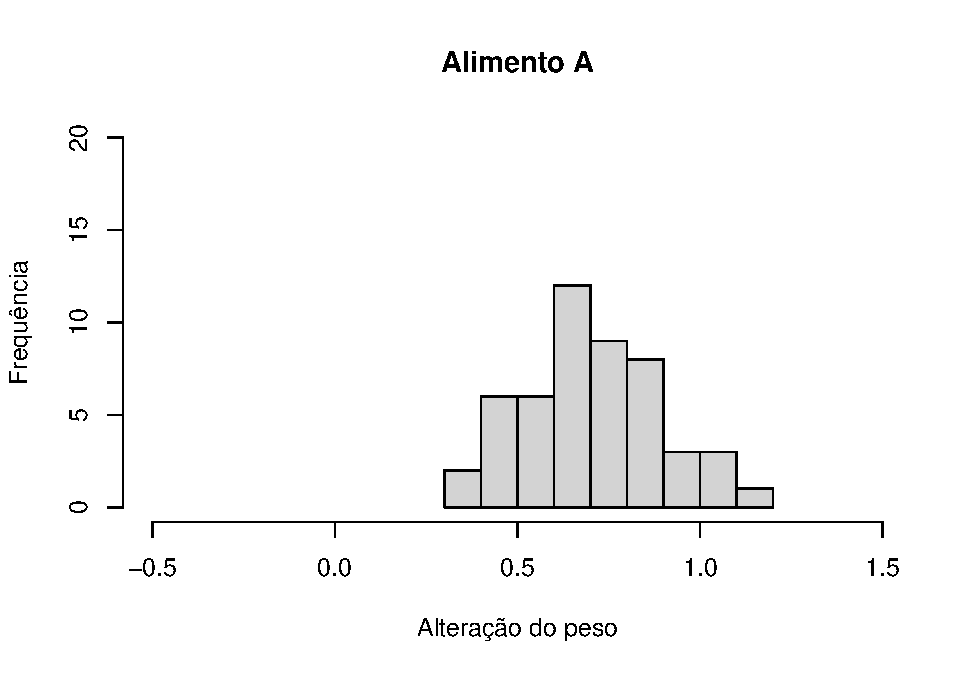
\includegraphics[width=0.7\linewidth]{livroR-1.0_files/figure-latex/hist-ali-A-1} 

}

\caption{Histograma com valores da mudança do peso dos gastrópodes após a dieta com o Alimento A}\label{fig:hist-ali-A}
\end{figure}

\begin{Shaded}
\begin{Highlighting}[]
\KeywordTok{hist}\NormalTok{(gastropode}\OperatorTok{$}\NormalTok{Peso [gastropode}\OperatorTok{$}\NormalTok{Alimento }\OperatorTok{==}\StringTok{ "Alimento B"}\NormalTok{], }
     \DataTypeTok{xlab =} \StringTok{"Alteração do peso"}\NormalTok{, }
     \DataTypeTok{ylab =} \StringTok{"Frequência", }
\StringTok{     main = "}\NormalTok{Alimento B}\StringTok{",}
\StringTok{     ylim = c(0, 20),}
\StringTok{     xlim = c(-0.5, 1.5))}
\end{Highlighting}
\end{Shaded}

\begin{figure}[H]

{\centering 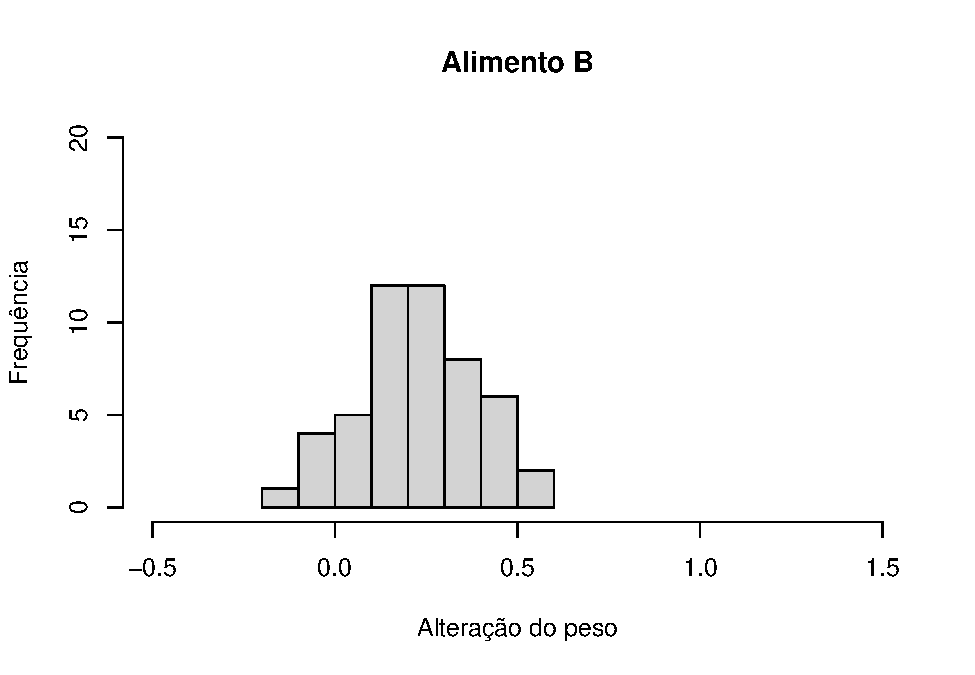
\includegraphics[width=0.7\linewidth]{livroR-1.0_files/figure-latex/hist-ali-B-1} 

}

\caption{Histograma com valores da mudança do peso dos gastrópodes após a dieta com o Alimento B}\label{fig:hist-ali-B}
\end{figure}

O Boxplot resume os dados por Alimento e nos indica outras métricas (quartis), como vimos anteriormente no tópico sobre gráficos.

\begin{Shaded}
\begin{Highlighting}[]
\KeywordTok{boxplot}\NormalTok{(Peso }\OperatorTok{~}\StringTok{ }\NormalTok{Alimento, }\DataTypeTok{data =}\NormalTok{ gastropode)}
\end{Highlighting}
\end{Shaded}

\begin{figure}[H]

{\centering 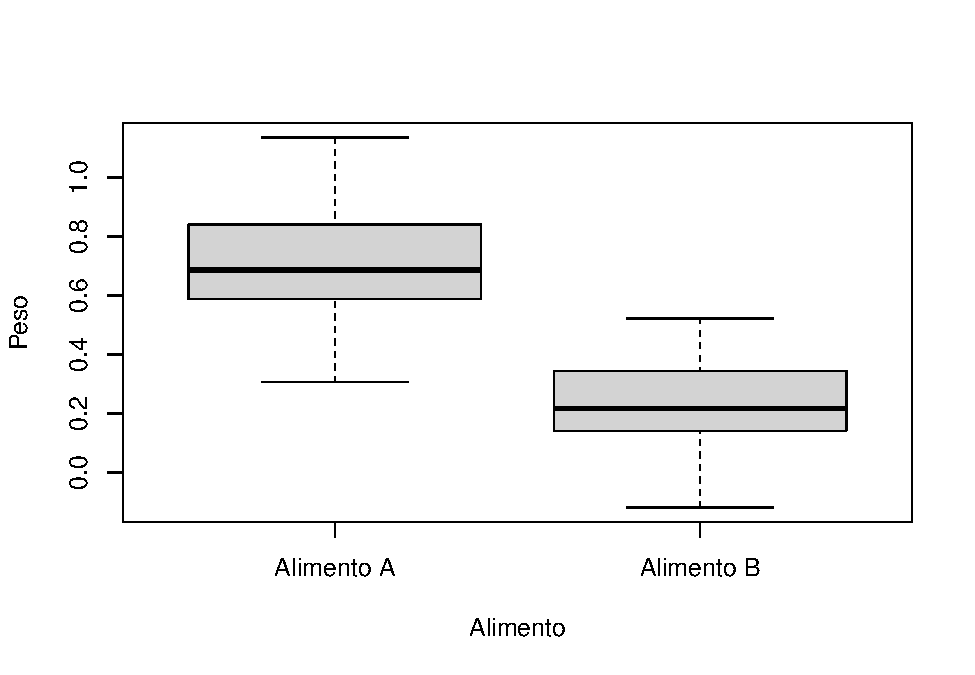
\includegraphics[width=0.7\linewidth]{livroR-1.0_files/figure-latex/box-ali-1} 

}

\caption{Boxplot com os valores da alteração do peso dos gastrópodes por tipo de alimento}\label{fig:box-ali}
\end{figure}

Mas se desejarmos observar os valores numéricos que resumem os dados, podemos seguir o que aprendemos anteriormente.

\begin{Shaded}
\begin{Highlighting}[]
\KeywordTok{summary}\NormalTok{(gastropode)}
\end{Highlighting}
\end{Shaded}

\begin{verbatim}
##        Alimento       Peso        
##  Alimento A:50   Min.   :-0.1180  
##  Alimento B:50   1st Qu.: 0.2172  
##                  Median : 0.4475  
##                  Mean   : 0.4652  
##                  3rd Qu.: 0.6843  
##                  Max.   : 1.1340
\end{verbatim}

\begin{Shaded}
\begin{Highlighting}[]
\KeywordTok{mean}\NormalTok{(gastropode}\OperatorTok{$}\NormalTok{Peso)}
\end{Highlighting}
\end{Shaded}

\begin{verbatim}
## [1] 0.46519
\end{verbatim}

\begin{Shaded}
\begin{Highlighting}[]
\KeywordTok{mean}\NormalTok{(gastropode}\OperatorTok{$}\NormalTok{Peso [gastropode}\OperatorTok{$}\NormalTok{Alimento }\OperatorTok{==}\StringTok{ "Alimento A"}\NormalTok{])}
\end{Highlighting}
\end{Shaded}

\begin{verbatim}
## [1] 0.7069
\end{verbatim}

\begin{Shaded}
\begin{Highlighting}[]
\KeywordTok{mean}\NormalTok{(gastropode}\OperatorTok{$}\NormalTok{Peso [gastropode}\OperatorTok{$}\NormalTok{Alimento }\OperatorTok{==}\StringTok{ "Alimento B"}\NormalTok{])}
\end{Highlighting}
\end{Shaded}

\begin{verbatim}
## [1] 0.22348
\end{verbatim}

Utilizando o pacote \textcolor{brown}{Rmisc} temos uma forma mais simples de escrita e eficiente para observar esses valores e algumas outras métricas.

\textcolor{red}{OBS: Não se esqueça de carregar o pacote por meio da função} \textcolor{blue}{library()}\textcolor{red}{.}

\begin{Shaded}
\begin{Highlighting}[]
\KeywordTok{library}\NormalTok{(Rmisc)}
\KeywordTok{summarySE}\NormalTok{(}\DataTypeTok{data =}\NormalTok{ gastropode, }\DataTypeTok{measurevar =} \StringTok{"Peso"}\NormalTok{, }\DataTypeTok{groupvars =} \StringTok{"Alimento"}\NormalTok{)}
\end{Highlighting}
\end{Shaded}

\begin{verbatim}
##     Alimento  N    Peso        sd         se         ci
## 1 Alimento A 50 0.70690 0.1852070 0.02619223 0.05263525
## 2 Alimento B 50 0.22348 0.1573551 0.02225337 0.04471982
\end{verbatim}

Até o momento observamos como estão os nossos dados e podemos ver que a administração do ``Alimento A'' resultou em um maior ganho de peso pelos gastropodes do que a ``Alimento B''. Mas será que o que observamos grafica e numericamente se reflete estatisticamente? Vamos a nossa avaliação dos pressupostos do teste-t para duas amostras e se cumpridos vamos para o teste-t.

Uma das formas mais convencionais de avaliar a normalidade é pelo teste de Shapiro-Wilks aplicando a função \textcolor{blue}{shapiro.test()} e a homocedasticidade pelo teste de Bartlett \textcolor{blue}{bartlett.test()}. Para o teste de normalidade de Shapiro-Wilks devemos aplica-lo à variável númerica desejada (ex: Peso) e realiza-lo para cada categória (ex: ``Alimento A'' e ``Alimento B'') da variável categorica escolhida (ex: Alimento) separadamente. Para o teste de homocedasticidade de Bartlett devemos avaliar a variável mensurável (ex: Peso) em função da variável categorica (ex: Alimento). Veja os comandos e resultado abaixo.

\begin{Shaded}
\begin{Highlighting}[]
\KeywordTok{shapiro.test}\NormalTok{(gastropode}\OperatorTok{$}\NormalTok{Peso [gastropode}\OperatorTok{$}\NormalTok{Alimento }\OperatorTok{==}\StringTok{ "Alimento A"}\NormalTok{])}
\end{Highlighting}
\end{Shaded}

\begin{verbatim}
## 
##  Shapiro-Wilk normality test
## 
## data:  gastropode$Peso[gastropode$Alimento == "Alimento A"]
## W = 0.98923, p-value = 0.9266
\end{verbatim}

\begin{Shaded}
\begin{Highlighting}[]
\KeywordTok{shapiro.test}\NormalTok{(gastropode}\OperatorTok{$}\NormalTok{Peso [gastropode}\OperatorTok{$}\NormalTok{Alimento }\OperatorTok{==}\StringTok{ "Alimento B"}\NormalTok{])}
\end{Highlighting}
\end{Shaded}

\begin{verbatim}
## 
##  Shapiro-Wilk normality test
## 
## data:  gastropode$Peso[gastropode$Alimento == "Alimento B"]
## W = 0.98059, p-value = 0.5769
\end{verbatim}

\begin{Shaded}
\begin{Highlighting}[]
\KeywordTok{bartlett.test}\NormalTok{(Peso }\OperatorTok{~}\StringTok{ }\NormalTok{Alimento, }\DataTypeTok{data =}\NormalTok{ gastropode)}
\end{Highlighting}
\end{Shaded}

\begin{verbatim}
## 
##  Bartlett test of homogeneity of variances
## 
## data:  Peso by Alimento
## Bartlett's K-squared = 1.2826, df = 1, p-value = 0.2574
\end{verbatim}

Como podemos observar, ambos os grupos apresentam dados normais e homocedásticos, para um nível de confiança de 95\%, já que o \emph{p-value} foi superior a 0,05. Dessa forma vamos dar continuidade a nossa análise e verificar se as médias dos grupos são diferentes aplicando a já conhecida função \textcolor{blue}{t.test()}.

\begin{Shaded}
\begin{Highlighting}[]
\KeywordTok{t.test}\NormalTok{(Peso }\OperatorTok{~}\StringTok{ }\NormalTok{Alimento, }
       \DataTypeTok{data =}\NormalTok{ gastropode,}
       \DataTypeTok{var.equal =} \OtherTok{TRUE}\NormalTok{,}
       \DataTypeTok{conf.level =} \FloatTok{0.95}\NormalTok{)}
\end{Highlighting}
\end{Shaded}

\begin{verbatim}
## 
##  Two Sample t-test
## 
## data:  Peso by Alimento
## t = 14.065, df = 98, p-value < 2.2e-16
## alternative hypothesis: true difference in means is not equal to 0
## 95 percent confidence interval:
##  0.4152153 0.5516247
## sample estimates:
## mean in group Alimento A mean in group Alimento B 
##                  0.70690                  0.22348
\end{verbatim}

Repare que a forma da escrita se alterou um pouco. Mas como podem ver, nada complicado. Agora escrevemos a variável mensurável (Peso) em função da (\textasciitilde{}) variável categórica (Alimento). Guarde bem essa forma de escrita (similar ao que realizamos no boxplot e barplot) pois ela será utilizada para praticamente todos os testes a partir daqui e para inúmeras outras funções. Adcionamos o argumento ``\emph{data}'' que indica a planilha de onde estamos utilizando as variáveis, o argumento ``\emph{var.equal}'' o qual indica que a variância entre os grupos é igual\footnote{por padrão o valor lógico para este argumento é FALSE e a função \textcolor{blue}{t.test()} realiza o teste de Welch)} e o argumento ``\emph{conf.level}'' o qual define o nível de confiança com qual estamos trabalhando.

De acordo com nosso resultado podemos ver que o valor do teste-t é 14,065, o grau de liberdade de 98 (o qual consiste no total de observações subtraído de um por grupo), o valor de probabilidade associado ao teste (\emph{p-value} = \(2,2\times10^{-16}\)), o intervalo de confiança de 95\% (0,415 e 0,551) que refere-se a diferença da média entre os grupos (a diferença da média dos grupos é: 0,70690 - 0,22348 = 0,48342), ou seja, o intervalo de confiança é em função dessa diferença e as últimas linhas do resultado representam as médias de alteração do peso para cada Alimento (Alimento A = 0,70690 e Alimento B = 0,22348). De acordo com esse resultado refutamos a hipótese nula de que as médias são similares. Portanto podemos dizer que dependendo do Alimento (A ou B) utilizada na dieta podemos ter diferentes alterações no peso dos gastropodes.

Da mesma forma que avaliamos para o teste-t de uma amostra, podemos plotar o resultado como um gráfico da função de densidade do teste-t. Só devemos lembrar de carregar o pacote \textcolor{brown}{webr}.

\begin{Shaded}
\begin{Highlighting}[]
\KeywordTok{library}\NormalTok{(webr)}
\KeywordTok{plot}\NormalTok{(}\KeywordTok{t.test}\NormalTok{(Peso }\OperatorTok{~}\StringTok{ }\NormalTok{Alimento, }
            \DataTypeTok{data =}\NormalTok{ gastropode,}
            \DataTypeTok{var.equal =} \OtherTok{TRUE}\NormalTok{,}
            \DataTypeTok{conf.level =} \FloatTok{0.95}\NormalTok{))}
\end{Highlighting}
\end{Shaded}

\begin{figure}[H]

{\centering 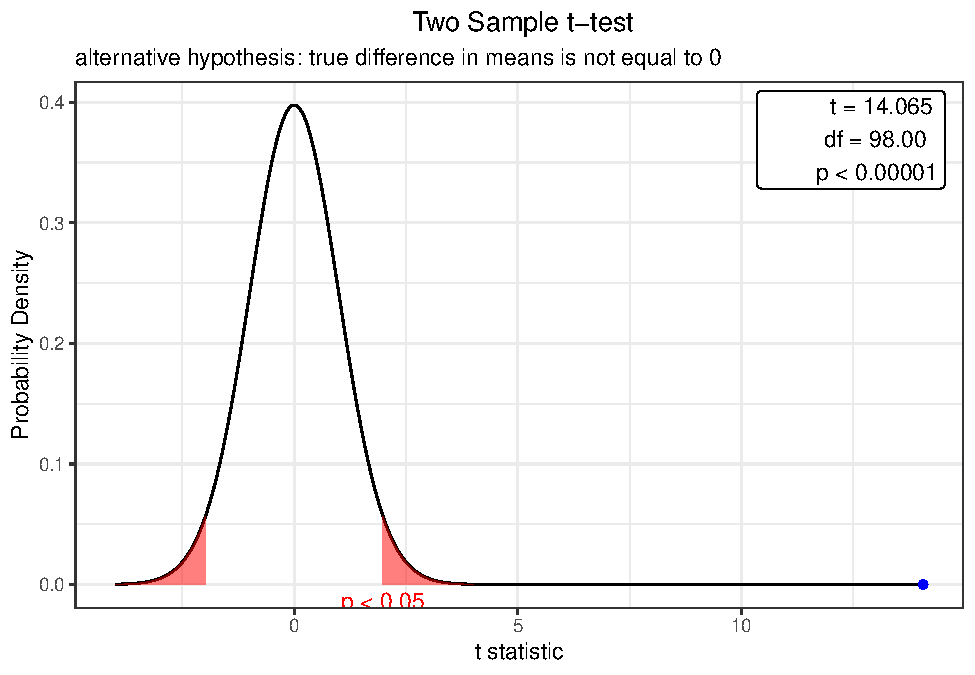
\includegraphics[width=0.7\linewidth]{livroR-1.0_files/figure-latex/testetduasdens-1} 

}

\caption{Curva de densidade representando o valor do teste-t bicaudal para a alteração do peso de gastrópodes em relação ao alimento a um intervalo de confiança de 95\%. O ponto azul indica o valor do teste.}\label{fig:testetduasdens}
\end{figure}

Neste gráfico podemos ver que o resultado do teste-t (Figura \ref{fig:testetduasdens}), indicado pelo ponto azul, está muito além do nível da zona de rejeição, indicando que os dois grupos apresentam médias bem diferentes, ou seja, a diferença entre as duas médias é altamente significativa.

Vamos exercitar nosso conhecimento em R e teste-t com um outro exemplo (Gere os dados abaixo).

\textcolor{red}{OBS: Neste momento não entraremos em detalhes sobre os comandos aplicados para construção dos dados.}

\begin{Shaded}
\begin{Highlighting}[]
\NormalTok{grupos <-}\StringTok{ }\KeywordTok{c}\NormalTok{(}\KeywordTok{rep}\NormalTok{(}\DataTypeTok{x =} \StringTok{"Ano 0"}\NormalTok{, }\DecValTok{36}\NormalTok{), }\KeywordTok{rep}\NormalTok{(}\DataTypeTok{x =} \StringTok{"Ano 20"}\NormalTok{, }\DecValTok{36}\NormalTok{))}
\KeywordTok{set.seed}\NormalTok{(}\DecValTok{245}\NormalTok{)}
\NormalTok{ano}\FloatTok{.0}\NormalTok{ <-}\StringTok{ }\KeywordTok{rnorm}\NormalTok{(}\DataTypeTok{n =} \DecValTok{36}\NormalTok{, }\DataTypeTok{mean =} \FloatTok{15.7}\NormalTok{, }\DataTypeTok{sd =} \FloatTok{0.2}\NormalTok{) }\OperatorTok{+}\StringTok{ }\KeywordTok{runif}\NormalTok{(}\DataTypeTok{n =} \DecValTok{36}\NormalTok{)}
\KeywordTok{set.seed}\NormalTok{(}\DecValTok{356}\NormalTok{)}
\NormalTok{ano}\FloatTok{.20}\NormalTok{ <-}\StringTok{ }\KeywordTok{rnorm}\NormalTok{(}\DataTypeTok{n =} \DecValTok{36}\NormalTok{, }\DataTypeTok{mean =} \FloatTok{16.2}\NormalTok{, }\DataTypeTok{sd =} \FloatTok{0.5}\NormalTok{) }\OperatorTok{+}\StringTok{ }\KeywordTok{runif}\NormalTok{(}\DataTypeTok{n =} \DecValTok{36}\NormalTok{)}
\NormalTok{ano <-}\StringTok{ }\KeywordTok{c}\NormalTok{(ano}\FloatTok{.0}\NormalTok{, ano}\FloatTok{.20}\NormalTok{)}
\NormalTok{lagoa <-}\StringTok{ }\KeywordTok{as.data.frame}\NormalTok{(}\KeywordTok{cbind}\NormalTok{(grupos, }\KeywordTok{round}\NormalTok{(ano, }\DecValTok{3}\NormalTok{)))}
\KeywordTok{colnames}\NormalTok{(lagoa) <-}\StringTok{ }\KeywordTok{c}\NormalTok{(}\StringTok{"Ano"}\NormalTok{, }\StringTok{"Temperatura"}\NormalTok{)}
\KeywordTok{rm}\NormalTok{(}\DataTypeTok{list =} \StringTok{"grupos"}\NormalTok{, }\StringTok{"ano.0"}\NormalTok{, }\StringTok{"ano.20"}\NormalTok{, }\StringTok{"ano"}\NormalTok{)}
\end{Highlighting}
\end{Shaded}

Imagine que durante um ano você mensurou a temperatura de uma lagoa três vezes por mês durante todos os meses ao longo de um ano. 20 anos depois você retornou a lagoa e mensurou novamente a temperatura três vezes por mês durante um ano. Considerando um nível de confiança de 99\% a temperatura é igual ou diferente entre os anos?

A primeira coisa que devemos fazer é escrever nossa hipótese. Vamos a ela.

\begin{itemize}
\tightlist
\item
  H0: A média da temperatura é igual entre os anos (\(\mu_{ano0} = \mu_{ano 20}\));
\item
  HA: A média da temperatura é diferente entre os anos (\(\mu_{ano0} \neq \mu_{ano 20}\));
\end{itemize}

Com a hipótese construída vamos verificar a estrutura dos dados (modificar se necessário) e sumarizar nossos dados grafica e estatisticamente. Conforme realizado no exemplo anterior.

Os comandos abaixo realizam a análise gráfica: o histograma dos valores de temperatura no ``ano 0'' (Figura \ref{fig:hist-temp-0}), o histograma dos valores de temperatura no ``ano 20'' (Figura \ref{fig:hist-temp-20}) e o boxplot para ambos os dados (Figura \ref{fig:box-temp}), respectivamente. Quanto ao seu resultado podemos notar uma maior temperatura média anual da lagoa 20 anos depois da primeira amostragem.

\begin{Shaded}
\begin{Highlighting}[]
\KeywordTok{head}\NormalTok{(lagoa)}
\end{Highlighting}
\end{Shaded}

\begin{verbatim}
##     Ano Temperatura
## 1 Ano 0      16.345
## 2 Ano 0      16.383
## 3 Ano 0      15.727
## 4 Ano 0      16.058
## 5 Ano 0      15.842
## 6 Ano 0      16.158
\end{verbatim}

\begin{Shaded}
\begin{Highlighting}[]
\KeywordTok{str}\NormalTok{(lagoa)}
\end{Highlighting}
\end{Shaded}

\begin{verbatim}
## 'data.frame':    72 obs. of  2 variables:
##  $ Ano        : chr  "Ano 0" "Ano 0" "Ano 0" "Ano 0" ...
##  $ Temperatura: chr  "16.345" "16.383" "15.727" "16.058" ...
\end{verbatim}

\begin{Shaded}
\begin{Highlighting}[]
\NormalTok{lagoa}\OperatorTok{$}\NormalTok{Ano <-}\StringTok{ }\KeywordTok{as.factor}\NormalTok{(lagoa}\OperatorTok{$}\NormalTok{Ano)}
\NormalTok{lagoa}\OperatorTok{$}\NormalTok{Temperatura <-}\StringTok{ }\KeywordTok{as.numeric}\NormalTok{(lagoa}\OperatorTok{$}\NormalTok{Temperatura)}
\KeywordTok{str}\NormalTok{(lagoa)}
\end{Highlighting}
\end{Shaded}

\begin{verbatim}
## 'data.frame':    72 obs. of  2 variables:
##  $ Ano        : Factor w/ 2 levels "Ano 0","Ano 20": 1 1 1 1 1 1 1 1 1 1 ...
##  $ Temperatura: num  16.3 16.4 15.7 16.1 15.8 ...
\end{verbatim}

\begin{Shaded}
\begin{Highlighting}[]
\KeywordTok{hist}\NormalTok{(lagoa}\OperatorTok{$}\NormalTok{Temperatura [lagoa}\OperatorTok{$}\NormalTok{Ano }\OperatorTok{==}\StringTok{ "Ano 0"}\NormalTok{], }
     \DataTypeTok{xlab =} \StringTok{"Temperatura (°C)"}\NormalTok{, }
     \DataTypeTok{ylab =} \StringTok{"Frequência", }
\StringTok{     main = "}\NormalTok{Ano }\DecValTok{0}\StringTok{", }
\StringTok{     ylim = c(0, 15),}
\StringTok{     xlim = c(15, 19))}
\end{Highlighting}
\end{Shaded}

\begin{figure}[H]

{\centering 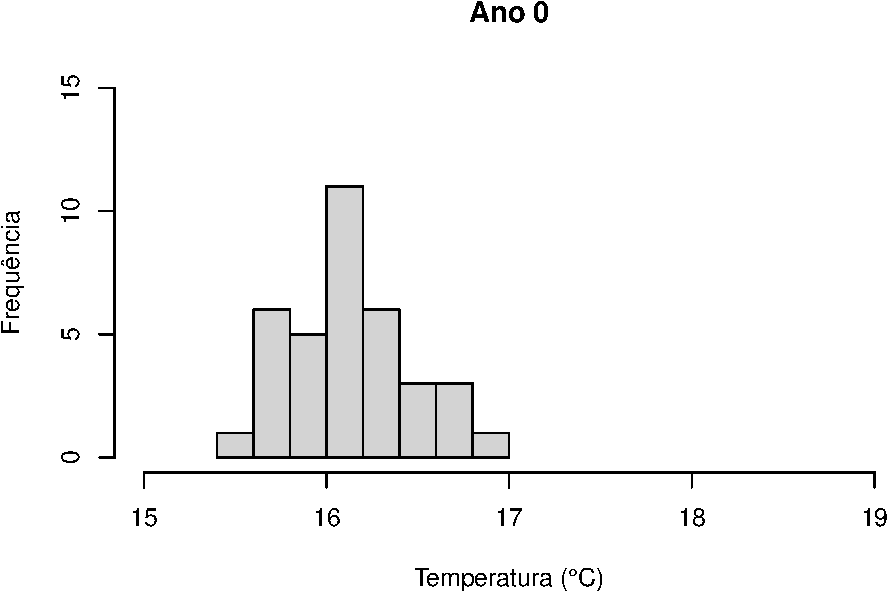
\includegraphics[width=0.7\linewidth]{livroR-1.0_files/figure-latex/hist-temp-0-1} 

}

\caption{Histograma com valores de temperatura da lagoa no Ano 0.}\label{fig:hist-temp-0}
\end{figure}

\begin{Shaded}
\begin{Highlighting}[]
\KeywordTok{hist}\NormalTok{(lagoa}\OperatorTok{$}\NormalTok{Temperatura [lagoa}\OperatorTok{$}\NormalTok{Ano }\OperatorTok{==}\StringTok{ "Ano 20"}\NormalTok{], }
     \DataTypeTok{xlab =} \StringTok{"Temperatura (°C)"}\NormalTok{, }
     \DataTypeTok{ylab =} \StringTok{"Frequência", }
\StringTok{     main = "}\NormalTok{Ano }\DecValTok{20}\StringTok{", }
\StringTok{     ylim = c(0, 15),}
\StringTok{     xlim = c(15, 19))}
\end{Highlighting}
\end{Shaded}

\begin{figure}[H]

{\centering 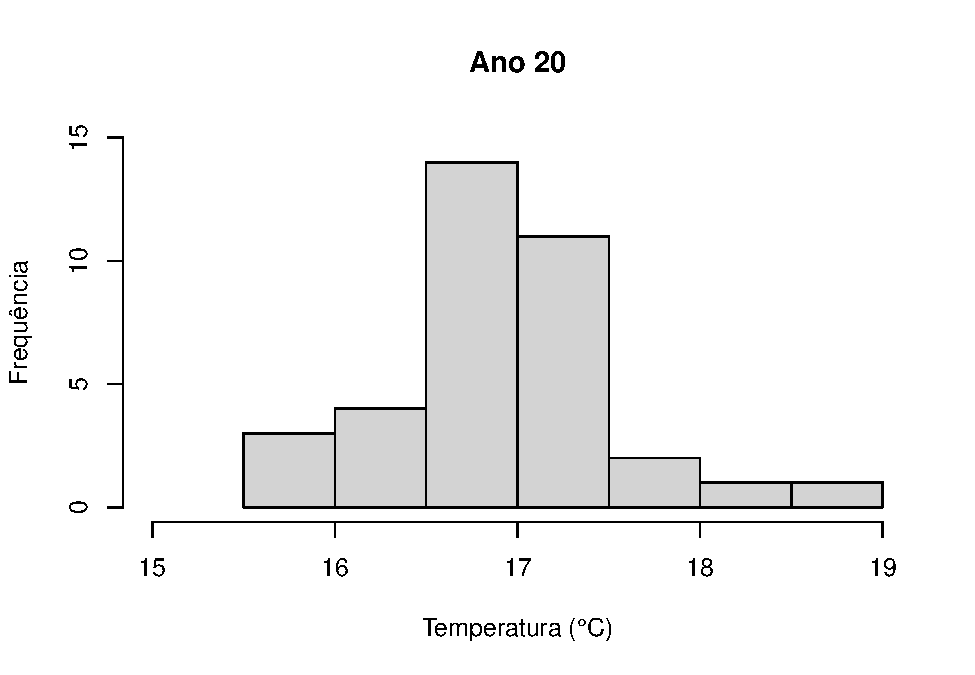
\includegraphics[width=0.7\linewidth]{livroR-1.0_files/figure-latex/hist-temp-20-1} 

}

\caption{Histograma com valores de temperatura da lagoa no Ano 20.}\label{fig:hist-temp-20}
\end{figure}

\begin{Shaded}
\begin{Highlighting}[]
\KeywordTok{boxplot}\NormalTok{(Temperatura }\OperatorTok{~}\StringTok{ }\NormalTok{Ano, }\DataTypeTok{data =}\NormalTok{ lagoa)}
\end{Highlighting}
\end{Shaded}

\begin{figure}[H]

{\centering 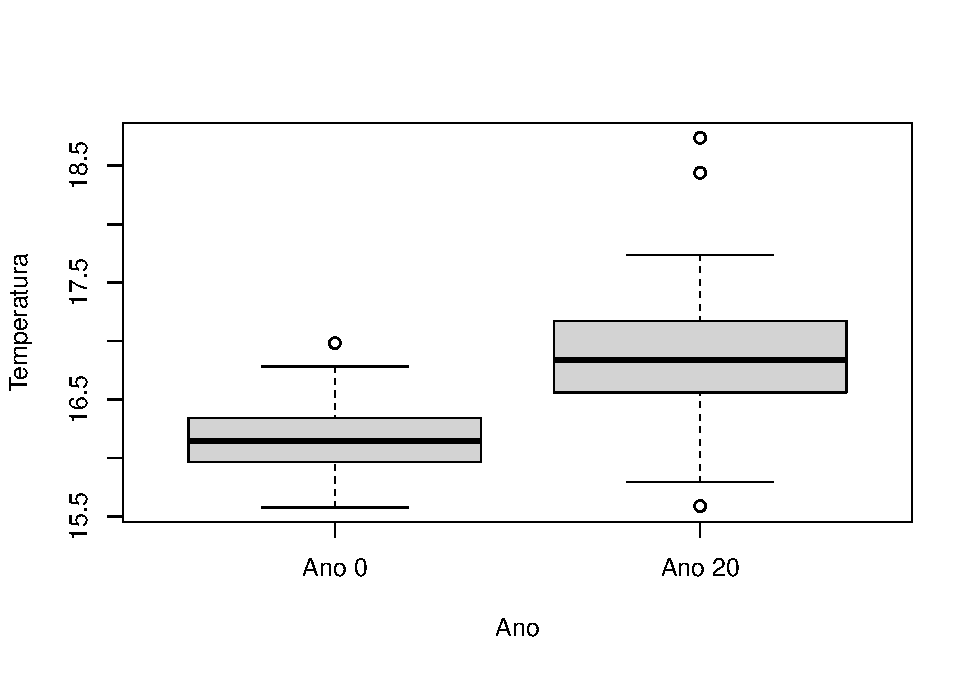
\includegraphics[width=0.7\linewidth]{livroR-1.0_files/figure-latex/box-temp-1} 

}

\caption{Boxplot com os valores de temperatura da lagoa por ano.}\label{fig:box-temp}
\end{figure}

Abaixo temos o comando para realizar a sumarização numérica dos dados.

\begin{Shaded}
\begin{Highlighting}[]
\KeywordTok{summary}\NormalTok{(lagoa)}
\end{Highlighting}
\end{Shaded}

\begin{verbatim}
##      Ano      Temperatura   
##  Ano 0 :36   Min.   :15.58  
##  Ano 20:36   1st Qu.:16.08  
##              Median :16.41  
##              Mean   :16.52  
##              3rd Qu.:16.86  
##              Max.   :18.74
\end{verbatim}

\begin{Shaded}
\begin{Highlighting}[]
\KeywordTok{library}\NormalTok{(Rmisc)}
\KeywordTok{summarySE}\NormalTok{(}\DataTypeTok{data =}\NormalTok{ lagoa, }\DataTypeTok{measurevar =} \StringTok{"Temperatura"}\NormalTok{, }\DataTypeTok{groupvars =} \StringTok{"Ano"}\NormalTok{)}
\end{Highlighting}
\end{Shaded}

\begin{verbatim}
##      Ano  N Temperatura        sd         se        ci
## 1  Ano 0 36    16.14661 0.3301591 0.05502652 0.1117098
## 2 Ano 20 36    16.89750 0.6409853 0.10683089 0.2168782
\end{verbatim}

Aplicando a função \textcolor{blue}{summarySE()} do pacote \textcolor{brown}{Rmisc} sumarizamos nossos dados como mostrado acima e em relação aos valores de média e desvios podemos observar que a média é bem próxima, mas será que elas são estatisticamente iguais? Para isso vamos realizar o teste-t.

Antes do teste-t vamos calcular os pressupostos requeridos, normalidade e homocedasticidade. Conforme realizado no exemplo anterior.

\begin{Shaded}
\begin{Highlighting}[]
\KeywordTok{shapiro.test}\NormalTok{(lagoa}\OperatorTok{$}\NormalTok{Temperatura [lagoa}\OperatorTok{$}\NormalTok{Ano }\OperatorTok{==}\StringTok{ "Ano 0"}\NormalTok{])}
\end{Highlighting}
\end{Shaded}

\begin{verbatim}
## 
##  Shapiro-Wilk normality test
## 
## data:  lagoa$Temperatura[lagoa$Ano == "Ano 0"]
## W = 0.97181, p-value = 0.4771
\end{verbatim}

\begin{Shaded}
\begin{Highlighting}[]
\KeywordTok{shapiro.test}\NormalTok{(lagoa}\OperatorTok{$}\NormalTok{Temperatura [lagoa}\OperatorTok{$}\NormalTok{Ano }\OperatorTok{==}\StringTok{ "Ano 20"}\NormalTok{])}
\end{Highlighting}
\end{Shaded}

\begin{verbatim}
## 
##  Shapiro-Wilk normality test
## 
## data:  lagoa$Temperatura[lagoa$Ano == "Ano 20"]
## W = 0.9571, p-value = 0.1747
\end{verbatim}

\begin{Shaded}
\begin{Highlighting}[]
\KeywordTok{bartlett.test}\NormalTok{(Temperatura }\OperatorTok{~}\StringTok{ }\NormalTok{Ano, }\DataTypeTok{data =}\NormalTok{ lagoa)}
\end{Highlighting}
\end{Shaded}

\begin{verbatim}
## 
##  Bartlett test of homogeneity of variances
## 
## data:  Temperatura by Ano
## Bartlett's K-squared = 14.189, df = 1, p-value = 0.0001653
\end{verbatim}

Como podemos ver os dados são normais, porém não são homocedasticos (a variância não é igual entre os grupos). Neste caso podemos fazer um teste-t de Welch (este teste aplica uma correção quando as variâncias não são iguais). Contudo, o teste de Welch ele é comumente usado quando o N amostral é considerado baixo (menor que 10 para um dos dois grupos). Vamos Analisar o teste-t considerando a variância igual e desigual para ver se há diferença significativa no resultado do teste ou não.

\begin{Shaded}
\begin{Highlighting}[]
\KeywordTok{t.test}\NormalTok{(Temperatura }\OperatorTok{~}\StringTok{ }\NormalTok{Ano, }
       \DataTypeTok{data =}\NormalTok{ lagoa,}
       \DataTypeTok{var.equal =} \OtherTok{TRUE}\NormalTok{,}
       \DataTypeTok{conf.level =} \FloatTok{0.99}\NormalTok{)}
\end{Highlighting}
\end{Shaded}

\begin{verbatim}
## 
##  Two Sample t-test
## 
## data:  Temperatura by Ano
## t = -6.2486, df = 70, p-value = 2.837e-08
## alternative hypothesis: true difference in means is not equal to 0
## 99 percent confidence interval:
##  -1.069087 -0.432691
## sample estimates:
##  mean in group Ano 0 mean in group Ano 20 
##             16.14661             16.89750
\end{verbatim}

\begin{Shaded}
\begin{Highlighting}[]
\KeywordTok{t.test}\NormalTok{(Temperatura }\OperatorTok{~}\StringTok{ }\NormalTok{Ano, }
       \DataTypeTok{data =}\NormalTok{ lagoa,}
       \DataTypeTok{var.equal =} \OtherTok{FALSE}\NormalTok{,}
       \DataTypeTok{conf.level =} \FloatTok{0.99}\NormalTok{)}
\end{Highlighting}
\end{Shaded}

\begin{verbatim}
## 
##  Welch Two Sample t-test
## 
## data:  Temperatura by Ano
## t = -6.2486, df = 52.35, p-value = 7.594e-08
## alternative hypothesis: true difference in means is not equal to 0
## 99 percent confidence interval:
##  -1.0721092 -0.4296686
## sample estimates:
##  mean in group Ano 0 mean in group Ano 20 
##             16.14661             16.89750
\end{verbatim}

Como podem notar a forma de escrever o teste é similar ao exemplo anterior as alterações consistem nas variáveis e no conjunto de dados utilizado e como foi pedido no teste a alteração do nível de confiança para 99\% (conf.level = 0,99) e os dois teste-t (com variância igual e com variância desigual - Welch).

Olhando para os dois resultados ambos os testes demonstraram diferenças significativas entre os anos, pois o \emph{p-value} foi menor que 0,01 (lembrar que como o nível de confiança foi alterado para 0,99 a significância só ocorrerá se o \emph{p-value} for menor que 0,01, como é o caso). Porém podemos ver que não há muita diferença em relação aos valores de ambos os testes-t, pois como ressaltamos a aplicação do teste de Welch apresenta maior peso quando as variâncias são desiguais e o número amostral de um dos grupos é muito pequeno (\textless{}10).

Assim como fizemos anteriormente vamos olhar o resultado em relação a distribuição da função de densidade do teste-t para um nível de confiança de 99\% (Figura \ref{fig:testet-duas-temp-dens}). Só devemos lembrar de carregar o pacote \textcolor{brown}{webr}, se ainda não foi carregado.

\begin{Shaded}
\begin{Highlighting}[]
\KeywordTok{library}\NormalTok{(webr)}
\KeywordTok{plot}\NormalTok{(}\KeywordTok{t.test}\NormalTok{(Temperatura }\OperatorTok{~}\StringTok{ }\NormalTok{Ano, }
            \DataTypeTok{data =}\NormalTok{ lagoa,}
            \DataTypeTok{var.equal =} \OtherTok{TRUE}\NormalTok{,}
            \DataTypeTok{conf.level =} \FloatTok{0.99}\NormalTok{))}
\end{Highlighting}
\end{Shaded}

\begin{figure}[H]

{\centering 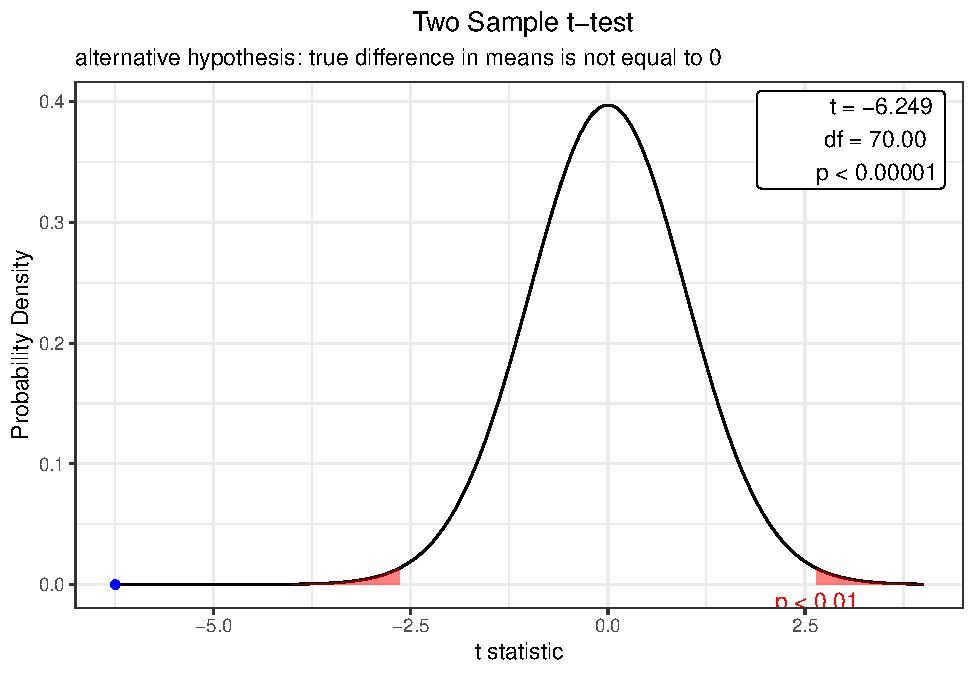
\includegraphics[width=0.7\linewidth]{livroR-1.0_files/figure-latex/testet-duas-temp-dens-1} 

}

\caption{Curva de densidade representando o valor do teste-t bicaudal para comparação da temperatura em um lago entre dois anos a um intervalo de confiança de 99\%. O ponto azul indica o valor do teste.}\label{fig:testet-duas-temp-dens}
\end{figure}

De acordo com esse exemplo podemos afirmar que os anos diferem entre si e que em 20 anos a lagoa amostrada apresentou um aumento da temperatura.

\hypertarget{teste-t-pareado}{%
\section{Teste-t pareado}\label{teste-t-pareado}}

Aplicamos este teste quando as duas amostras de uma variável categórica são independentes e desejamos verificar se os pares de observações entre os grupos diferem entre si (Tabela \ref{tab:tab3t}). Cada observação de ambas as amostras devem estar associadas para podermos dizer que ocorrem em pares.

\begin{table}

\caption{\label{tab:tab3t}Principais características do teste-t pareado}
\centering
\begin{tabular}[c]{>{\raggedright\arraybackslash}p{10em}>{\raggedright\arraybackslash}p{30em}}
\toprule
Atributos & Características\\
\midrule
\textbf{\cellcolor{gray!6}{Tipo de variável}} & \cellcolor{gray!6}{Quantitativa e categórica}\\
\textbf{Quantidade de variáveis} & 3 (1 quantitativa e 2 categóricas)\\
\textbf{\cellcolor{gray!6}{Hipótese nula}} & \cellcolor{gray!6}{A diferença na média da variável quantitativa entre os pares de grupos é igual a 0.}\\
\textbf{Fórmula} & $$t=\frac{\overline{d}}{s_{\overline{d}}}$$, onde, $\overline{d}$: média da diferença entre os pares de observações entre os grupos, $s_{\overline{d}}$: erro padrão da diferença entre os pares de observações entre os grupos.\\
\textbf{\cellcolor{gray!6}{Observação}} & \cellcolor{gray!6}{Não há a necessidade de post-hoc nem expressa-la graficamente.}\\
\bottomrule
\end{tabular}
\end{table}

Vejamos um exemplo de como conduzir essa análise.

Imagine que dois pesquisadores embarcaram com objetivo de fazer contagem de aves em alto mar. Após 20 dias de observações, independentes entre os observadores, obtivemos os dados abaixo.

Começaremos gerando os dados e o modificando conforme o necessário.

\textcolor{red}{OBS: Neste momento não entraremos em detalhes sobre os comandos aplicados para construção dos dados.}

\begin{Shaded}
\begin{Highlighting}[]
\KeywordTok{set.seed}\NormalTok{(}\DecValTok{2328}\NormalTok{)}
\NormalTok{aves}\FloatTok{.1}\NormalTok{ <-}\StringTok{ }\KeywordTok{rnorm}\NormalTok{(}\DataTypeTok{n =} \DecValTok{20}\NormalTok{, }\DataTypeTok{mean =} \DecValTok{20}\NormalTok{, }\DataTypeTok{sd =} \DecValTok{1}\NormalTok{) }\OperatorTok{+}\StringTok{ }\KeywordTok{runif}\NormalTok{(}\DataTypeTok{n =} \DecValTok{20}\NormalTok{)}
\KeywordTok{set.seed}\NormalTok{(}\DecValTok{3230}\NormalTok{)}
\NormalTok{aves}\FloatTok{.2}\NormalTok{ <-}\StringTok{ }\KeywordTok{rnorm}\NormalTok{(}\DataTypeTok{n =} \DecValTok{20}\NormalTok{, }\DataTypeTok{mean =} \DecValTok{21}\NormalTok{, }\DataTypeTok{sd =} \DecValTok{2}\NormalTok{) }\OperatorTok{+}\StringTok{ }\KeywordTok{runif}\NormalTok{(}\DataTypeTok{n =} \DecValTok{20}\NormalTok{)}
\NormalTok{dia <-}\StringTok{ }\KeywordTok{c}\NormalTok{(}\StringTok{"Dia 1"}\NormalTok{, }\StringTok{"Dia 2"}\NormalTok{, }\StringTok{"Dia 3"}\NormalTok{, }\StringTok{"Dia 4"}\NormalTok{, }\StringTok{"Dia 5"}\NormalTok{, }\StringTok{"Dia 6"}\NormalTok{, }\StringTok{"Dia 7"}\NormalTok{, }\StringTok{"Dia 8"}\NormalTok{, }
         \StringTok{"Dia 9"}\NormalTok{, }\StringTok{"Dia 10"}\NormalTok{, }\StringTok{"Dia 11"}\NormalTok{, }\StringTok{"Dia 12"}\NormalTok{, }\StringTok{"Dia 13"}\NormalTok{, }\StringTok{"Dia 14"}\NormalTok{, }\StringTok{"Dia 15"}\NormalTok{, }\StringTok{"Dia 16"}\NormalTok{,}
         \StringTok{"Dia 17"}\NormalTok{, }\StringTok{"Dia 18"}\NormalTok{, }\StringTok{"Dia 19"}\NormalTok{, }\StringTok{"Dia 20"}\NormalTok{)}
\NormalTok{aves <-}\StringTok{ }\KeywordTok{as.data.frame}\NormalTok{(}\KeywordTok{cbind}\NormalTok{(dia, }\KeywordTok{round}\NormalTok{(aves}\FloatTok{.1}\NormalTok{, }\DecValTok{0}\NormalTok{), }\KeywordTok{round}\NormalTok{(aves}\FloatTok{.2}\NormalTok{, }\DecValTok{0}\NormalTok{)))}
\KeywordTok{colnames}\NormalTok{(aves) <-}\StringTok{ }\KeywordTok{c}\NormalTok{(}\StringTok{"Dia"}\NormalTok{, }\StringTok{"Observador.1"}\NormalTok{, }\StringTok{"Observador.2"}\NormalTok{)}
\KeywordTok{rm}\NormalTok{(}\DataTypeTok{list =} \StringTok{"aves.1"}\NormalTok{, }\StringTok{"aves.2"}\NormalTok{, }\StringTok{"dia"}\NormalTok{)}
\end{Highlighting}
\end{Shaded}

Nestes casos temos as seguintes hipoteses:

\begin{itemize}
\tightlist
\item
  H0: A diferença na média do número de observações de aves entre os Observadores é igual a 0.
\item
  HA: A diferença na média do número de observações de aves entre os Observadores difere de 0.
\end{itemize}

Vamos verificar a estrutura dos dados e modificar conforme a necessidade.

\begin{Shaded}
\begin{Highlighting}[]
\KeywordTok{head}\NormalTok{(aves)}
\end{Highlighting}
\end{Shaded}

\begin{verbatim}
##     Dia Observador.1 Observador.2
## 1 Dia 1           19           20
## 2 Dia 2           20           22
## 3 Dia 3           18           23
## 4 Dia 4           22           18
## 5 Dia 5           22           22
## 6 Dia 6           22           23
\end{verbatim}

\begin{Shaded}
\begin{Highlighting}[]
\KeywordTok{str}\NormalTok{(aves)}
\end{Highlighting}
\end{Shaded}

\begin{verbatim}
## 'data.frame':    20 obs. of  3 variables:
##  $ Dia         : chr  "Dia 1" "Dia 2" "Dia 3" "Dia 4" ...
##  $ Observador.1: chr  "19" "20" "18" "22" ...
##  $ Observador.2: chr  "20" "22" "23" "18" ...
\end{verbatim}

\begin{Shaded}
\begin{Highlighting}[]
\NormalTok{aves}\OperatorTok{$}\NormalTok{Dia <-}\StringTok{ }\KeywordTok{as.factor}\NormalTok{(aves}\OperatorTok{$}\NormalTok{Dia)}
\NormalTok{aves}\OperatorTok{$}\NormalTok{Observador}\FloatTok{.1}\NormalTok{ <-}\StringTok{ }\KeywordTok{as.numeric}\NormalTok{(aves}\OperatorTok{$}\NormalTok{Observador}\FloatTok{.1}\NormalTok{)}
\NormalTok{aves}\OperatorTok{$}\NormalTok{Observador}\FloatTok{.2}\NormalTok{ <-}\StringTok{ }\KeywordTok{as.numeric}\NormalTok{(aves}\OperatorTok{$}\NormalTok{Observador}\FloatTok{.2}\NormalTok{)}
\KeywordTok{str}\NormalTok{(aves)}
\end{Highlighting}
\end{Shaded}

\begin{verbatim}
## 'data.frame':    20 obs. of  3 variables:
##  $ Dia         : Factor w/ 20 levels "Dia 1","Dia 10",..: 1 12 14 15 16 17 18 19 20 2 ...
##  $ Observador.1: num  19 20 18 22 22 22 21 20 22 21 ...
##  $ Observador.2: num  20 22 23 18 22 23 20 24 22 24 ...
\end{verbatim}

Neste exemplo podemos perceber que temos as variáveis categóricas ``Dia'' e observadores os quais estão em colunas como: ``Observador 1'' e ``Observador 2'' e a variável quantitativa ``aves'' que consiste no número de aves avistadas.

Vamos sumarizar os dados grafica e estatisticamente.

Primeiro vejamos nossos histogramas relativos a observações em relação aos observadores (Figura \ref{fig:hist-par-obs1} e \ref{fig:hist-par-obs2}).

\begin{Shaded}
\begin{Highlighting}[]
\KeywordTok{hist}\NormalTok{(aves}\OperatorTok{$}\NormalTok{Observador}\FloatTok{.1}\NormalTok{, }
     \DataTypeTok{xlab =} \StringTok{"Observações"}\NormalTok{, }
     \DataTypeTok{ylab =} \StringTok{"Frequência", }
\StringTok{     main = "}\NormalTok{Observador }\DecValTok{1}\StringTok{", }
\StringTok{     ylim = c(0, 10),}
\StringTok{     xlim = c(18, 25))}
\end{Highlighting}
\end{Shaded}

\begin{figure}[H]

{\centering 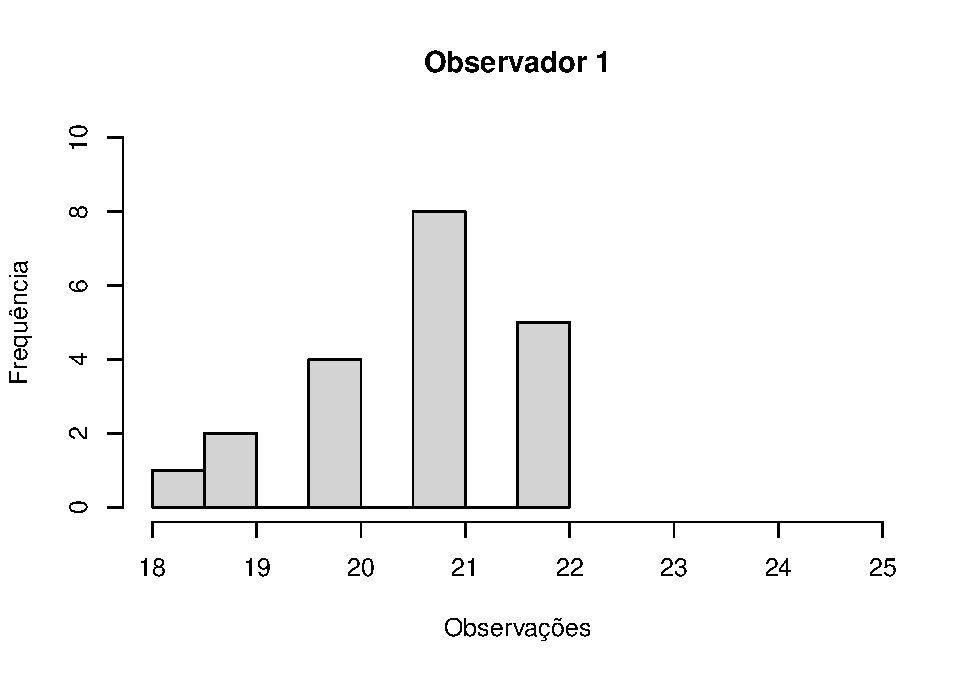
\includegraphics[width=0.7\linewidth]{livroR-1.0_files/figure-latex/hist-par-obs1-1} 

}

\caption{Histograma com a frequência de observações de aves, por 20 dias, pelo observador 1}\label{fig:hist-par-obs1}
\end{figure}

\begin{Shaded}
\begin{Highlighting}[]
\KeywordTok{hist}\NormalTok{(aves}\OperatorTok{$}\NormalTok{Observador}\FloatTok{.2}\NormalTok{, }
     \DataTypeTok{xlab =} \StringTok{"Observações"}\NormalTok{, }
     \DataTypeTok{ylab =} \StringTok{"Frequência", }
\StringTok{     main = "}\NormalTok{Observador }\DecValTok{2}\StringTok{", }
\StringTok{     ylim = c(0, 10),}
\StringTok{     xlim = c(18, 25))}
\end{Highlighting}
\end{Shaded}

\begin{figure}[H]

{\centering 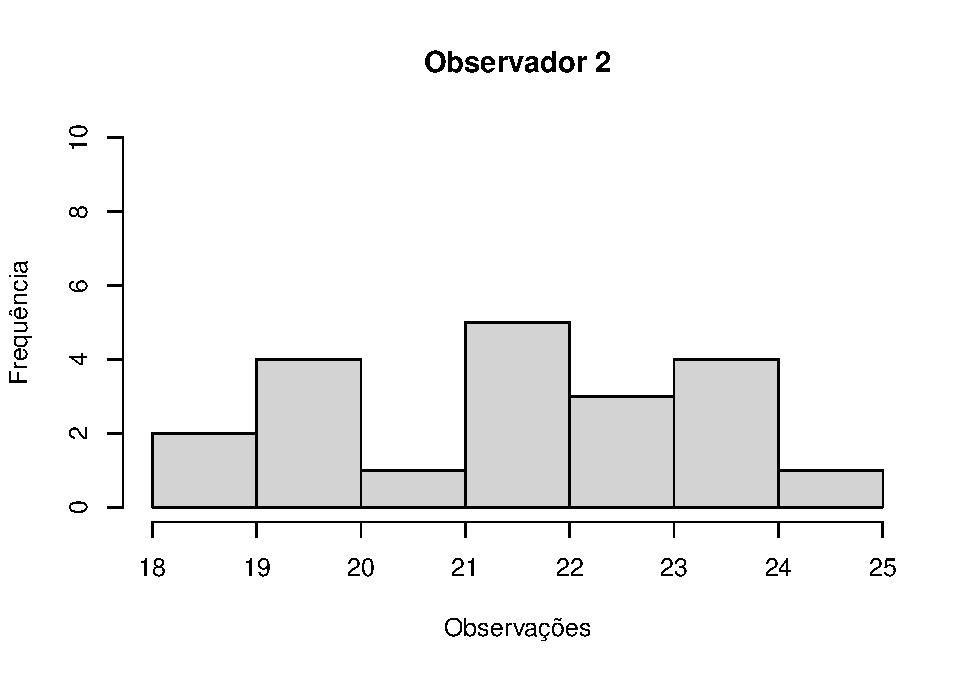
\includegraphics[width=0.7\linewidth]{livroR-1.0_files/figure-latex/hist-par-obs2-1} 

}

\caption{Histograma com a frequência de observações de aves, por 20 dias, pelo observador 2}\label{fig:hist-par-obs2}
\end{figure}

Agora vejamos o boxplot, repare que neste caso a sua escrita difere um pouco do que fizemos nos exemplos anteriores, pois agora inserimos a coluna referente ao ``Observador 1'' e depois a coluna referente ao ``Observador 2'' ((Figura \ref{fig:box-par-ave}). Isso se deve ao fato da planilha estar estruturada de forma diferente das anteriores. Não utilizamos o til (\textasciitilde{}), mas inserimos o nome da planilha seguido pelo operador matemático ``\textbf{\$}'' (cifrão) mais o nome da variável quantitativa que queremos representar. Inserimos também outros 2 argumentos que são ``\emph{names}'' com dois nomes concatenados pela função \textcolor{blue}{c()} que representam as variaveis quantitativas na ordem em que foram inseridas e o argumento ``ylab'' que dá nome ao eixo y.

\begin{Shaded}
\begin{Highlighting}[]
\KeywordTok{boxplot}\NormalTok{(aves}\OperatorTok{$}\NormalTok{Observador}\FloatTok{.1}\NormalTok{, }
\NormalTok{        aves}\OperatorTok{$}\NormalTok{Observador}\FloatTok{.2}\NormalTok{, }
        \DataTypeTok{names =} \KeywordTok{c}\NormalTok{(}\StringTok{"Observador 1"}\NormalTok{, }\StringTok{"Observador 2"}\NormalTok{),}
        \DataTypeTok{ylab =} \StringTok{"Frequência de Observações"}\NormalTok{)}
\end{Highlighting}
\end{Shaded}

\begin{figure}[H]

{\centering 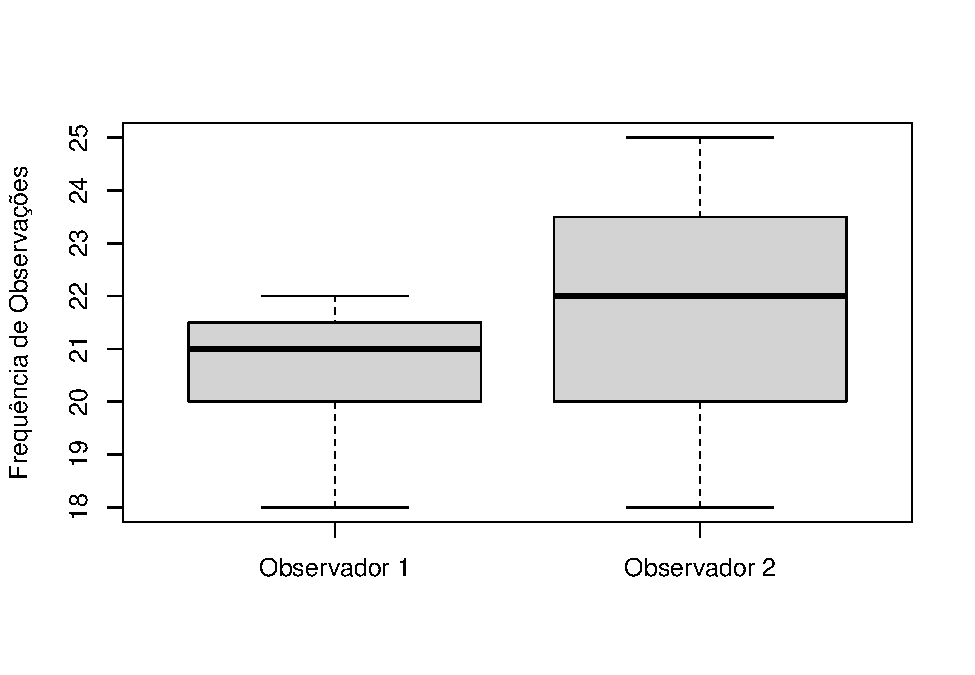
\includegraphics[width=0.7\linewidth]{livroR-1.0_files/figure-latex/box-par-ave-1} 

}

\caption{Boxplot com as frequências de observações de aves por 20 dias de 2 observadores.}\label{fig:box-par-ave}
\end{figure}

Vejamos o o resumo de nossos dados utilizando a função padrão do R \textcolor{blue}{summary}.

\begin{Shaded}
\begin{Highlighting}[]
\KeywordTok{summary}\NormalTok{(aves)}
\end{Highlighting}
\end{Shaded}

\begin{verbatim}
##       Dia      Observador.1    Observador.2  
##  Dia 1  : 1   Min.   :18.00   Min.   :18.00  
##  Dia 10 : 1   1st Qu.:20.00   1st Qu.:20.00  
##  Dia 11 : 1   Median :21.00   Median :22.00  
##  Dia 12 : 1   Mean   :20.70   Mean   :21.90  
##  Dia 13 : 1   3rd Qu.:21.25   3rd Qu.:23.25  
##  Dia 14 : 1   Max.   :22.00   Max.   :25.00  
##  (Other):14
\end{verbatim}

Como podemos notar, devido a organização dos dados na planilha a função \textcolor{blue}{summary()} já resume de maneira adequada nossos dados.

Em relação ao resumo dos nossos dados temos que o observador 2 contabilizou um número maior de aves que o observador 1, mas será que a diferença nos pares de observações é zero? De outra maneira, será que a média da diferença entre os pares de obsevações de aves entre os observadores é similar?

O teste-t pareado não apresenta pressuposto quanto aos dados, porém como ele avalia a diferença entre dois grupos o pressuposto requerido é a normalidade da diferença dos dados. Vamos a nossa avaliação do pressuposto.

Primeiro vamos criar um objeto que consiste na diferença entre observadores

\begin{Shaded}
\begin{Highlighting}[]
\NormalTok{diferenca <-}\StringTok{ }\NormalTok{aves}\OperatorTok{$}\NormalTok{Observador}\FloatTok{.1} \OperatorTok{-}\StringTok{ }\NormalTok{aves}\OperatorTok{$}\NormalTok{Observador}\FloatTok{.2}
\end{Highlighting}
\end{Shaded}

Agora vamos realizar o teste de normalidade da diferença.

\begin{Shaded}
\begin{Highlighting}[]
\KeywordTok{shapiro.test}\NormalTok{(diferenca)}
\end{Highlighting}
\end{Shaded}

\begin{verbatim}
## 
##  Shapiro-Wilk normality test
## 
## data:  diferenca
## W = 0.98173, p-value = 0.9544
\end{verbatim}

De acordo com o teste de Shapiro os dados são normais. Vamos a nossa avaliação pelo teste-t.

\begin{Shaded}
\begin{Highlighting}[]
\KeywordTok{t.test}\NormalTok{(aves}\OperatorTok{$}\NormalTok{Observador}\FloatTok{.1}\NormalTok{,}
\NormalTok{       aves}\OperatorTok{$}\NormalTok{Observador}\FloatTok{.2}\NormalTok{,}
       \DataTypeTok{paired =} \OtherTok{TRUE}\NormalTok{,}
       \DataTypeTok{conf.level =} \FloatTok{0.95}\NormalTok{)}
\end{Highlighting}
\end{Shaded}

\begin{verbatim}
## 
##  Paired t-test
## 
## data:  aves$Observador.1 and aves$Observador.2
## t = -2.1608, df = 19, p-value = 0.04369
## alternative hypothesis: true difference in means is not equal to 0
## 95 percent confidence interval:
##  -2.36237491 -0.03762509
## sample estimates:
## mean of the differences 
##                    -1.2
\end{verbatim}

Para a execução do teste-t pareado 2 diferenças podem ser notadas na escrita da função, em relação ao teste-t para duas amostras. A primeira consiste no fato de que não utilizamos o til (\textasciitilde{}), mas sim as variáveis referentes as observações e a segunda é o argumento ``\emph{paired}'' que tem valor lógico (ou seja, TRUE ou FALSE) e indicamos ele como ``TRUE'' (verdadeiro).

Quanto ao resultado podemos notar que nos é informado que o teste consiste num teste-t pareado e que o número de aves observadas pelos observadores é ligeiramente diferente a um nível de confiança de 95\%, visto que o \emph{p-value} é próximo à 0,05 e na última linha nos é indicado que a média da diferença das observações é de -1,2. Em outras palavras o teste nos diz que a média das diferenças nas observações de aves é diferente de 0\footnote{Zero (0) indica igualdade no número de observações.}, portanto rejeitamos a hipótese nula.

Assim como fizemos anteriormente vamos olhar o resultado em relação a distribuição função de densidade do teste-t (Figura \ref{fig:testet-par-ave}). Só devemos lembrar de carregar o pacote \textcolor{brown}{webr} se ainda não foi carregado.

\begin{Shaded}
\begin{Highlighting}[]
\KeywordTok{library}\NormalTok{(webr)}
\KeywordTok{plot}\NormalTok{(}\KeywordTok{t.test}\NormalTok{(aves}\OperatorTok{$}\NormalTok{Observador}\FloatTok{.1}\NormalTok{,}
\NormalTok{            aves}\OperatorTok{$}\NormalTok{Observador}\FloatTok{.2}\NormalTok{,}
            \DataTypeTok{paired =} \OtherTok{TRUE}\NormalTok{,}
            \DataTypeTok{conf.level =} \FloatTok{0.95}\NormalTok{))}
\end{Highlighting}
\end{Shaded}

\begin{figure}[H]

{\centering 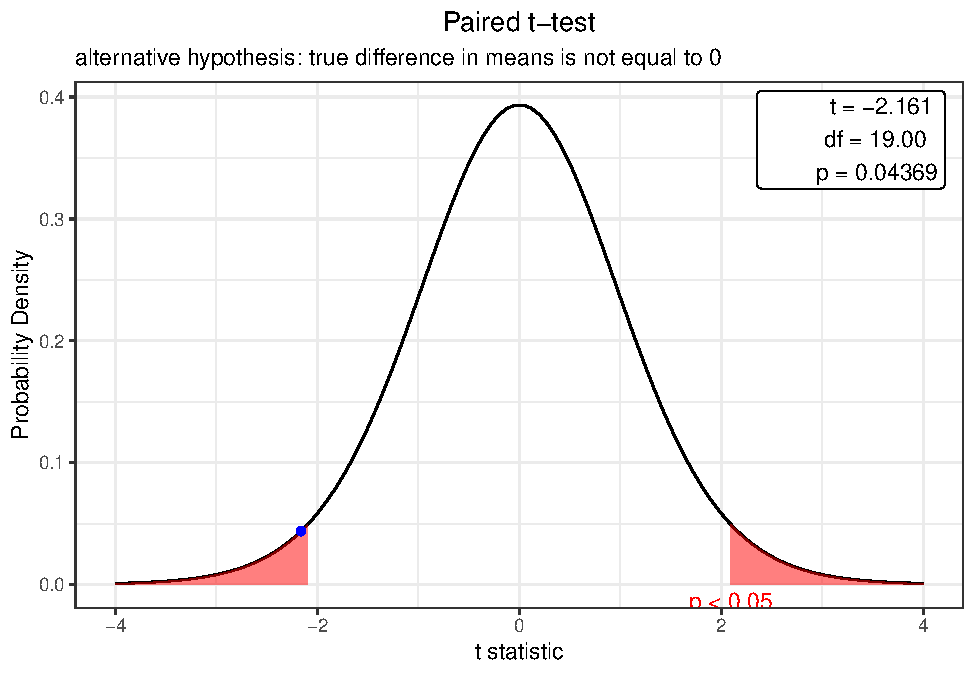
\includegraphics[width=0.7\linewidth]{livroR-1.0_files/figure-latex/testet-par-ave-1} 

}

\caption{Curva de densidade representando o valor do teste-t bicaudal para comparação do número de observações de aves por 2 observadores distintos a um intervalo de confiança de 95\%. O ponto azul indica o valor do teste.}\label{fig:testet-par-ave}
\end{figure}

Neste teste em particular como trabalhamos com a diferença entre as observações podemos usar o gráfico de barras para graficar essa diferença.

Para o gráfico indicaremos em seu comando que faremos um gráfico de barras onde o que será plotado é o objeto que consiste na diferença entre o número de observação de aves entre observadores (objeto: \textbf{diferenca}) (Figura \ref{fig:bar-dif-ave}). O argumento ``xlab'' indica o nome do eixo x, ``ylab'' o nome do eixo y, ``\emph{main}'' indica o título do gráfico, ``\emph{names.arg}'' indica a coluna referente aos nomes das barras (que são os dias), ``las'' indica se os nomes das barras serão plotados na horizontal ou vertical (o valor 2 indica vertical), ``ylim'' indica os limites do eixo y e ``\emph{cex.names}'' indica o tamanho da letra dos nomes das barras.

\begin{Shaded}
\begin{Highlighting}[]
\KeywordTok{barplot}\NormalTok{(diferenca,}
        \DataTypeTok{xlab =} \StringTok{"Dias"}\NormalTok{,}
        \DataTypeTok{ylab =} \StringTok{"Diferença entre observadores (Observador 1 - Observador 2)"}\NormalTok{,}
        \DataTypeTok{main =} \StringTok{"Meu gráfico"}\NormalTok{,}
        \DataTypeTok{names.arg =}\NormalTok{ aves}\OperatorTok{$}\NormalTok{Dia,}
        \DataTypeTok{las =} \DecValTok{2}\NormalTok{,}
        \DataTypeTok{ylim =} \KeywordTok{c}\NormalTok{(}\OperatorTok{-}\FloatTok{7.3}\NormalTok{, }\FloatTok{7.3}\NormalTok{),}
        \DataTypeTok{cex.names =} \FloatTok{0.9}\NormalTok{)}
\end{Highlighting}
\end{Shaded}

\begin{figure}[H]

{\centering 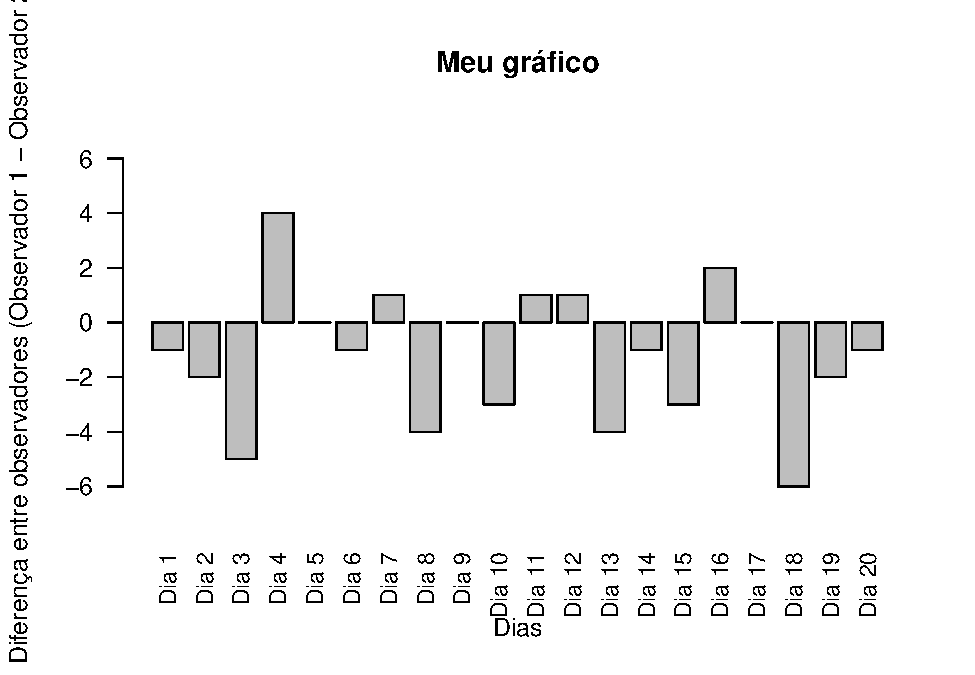
\includegraphics[width=0.7\linewidth]{livroR-1.0_files/figure-latex/bar-dif-ave-1} 

}

\caption{Diferença entre o número de observações de aves, por dia, para cada observador}\label{fig:bar-dif-ave}
\end{figure}

As barras para o lado positivo do eixo y indica uma maior observação de aves pelo ``Observador 1'' e as barras para baixo indicam um maior número de observações de aves pelo ``Observador 2''. Vamos indicar isso no gráfico por meio da função \textcolor{blue}{mtext()} (Figura \ref{fig:bar-dif-ave2}).

\begin{Shaded}
\begin{Highlighting}[]
\KeywordTok{barplot}\NormalTok{(diferenca,}
        \DataTypeTok{xlab =} \StringTok{"Dias"}\NormalTok{,}
        \DataTypeTok{ylab =} \StringTok{"Diferença entre observadores (Observador 1 - Observador 2)"}\NormalTok{,}
        \DataTypeTok{main =} \StringTok{"Meu gráfico"}\NormalTok{,}
        \DataTypeTok{names.arg =}\NormalTok{ aves}\OperatorTok{$}\NormalTok{Dia,}
        \DataTypeTok{las =} \DecValTok{2}\NormalTok{,}
        \DataTypeTok{ylim =} \KeywordTok{c}\NormalTok{(}\OperatorTok{-}\FloatTok{7.3}\NormalTok{, }\FloatTok{7.3}\NormalTok{),}
        \DataTypeTok{cex.names =} \FloatTok{0.9}\NormalTok{)}
\KeywordTok{mtext}\NormalTok{(}\DataTypeTok{at =} \DecValTok{4}\NormalTok{,}
      \DataTypeTok{line =} \DecValTok{-2}\NormalTok{,}
      \DataTypeTok{text =} \StringTok{"Observador 1"}\NormalTok{, }
      \DataTypeTok{side =} \DecValTok{3}\NormalTok{)}
\KeywordTok{mtext}\NormalTok{(}\DataTypeTok{at =} \DecValTok{4}\NormalTok{, }
      \DataTypeTok{line =} \DecValTok{-2}\NormalTok{,}
      \DataTypeTok{text =} \StringTok{"Observador 2"}\NormalTok{, }
      \DataTypeTok{side =} \DecValTok{1}\NormalTok{)}
\end{Highlighting}
\end{Shaded}

\begin{figure}[H]

{\centering \includegraphics[width=0.7\linewidth]{livroR-1.0_files/figure-latex/bar-dif-ave2-1} 

}

\caption{Diferença entre o número de observações de aves, por dia, para cada observador.}\label{fig:bar-dif-ave2}
\end{figure}

Como podem visualizar a função \textcolor{blue}{mtext()} indicou os nomes ``Observador 1'' e ``Observador 2'' no lado do gráfico que os representa. O argumento ``at'' indica a posição em relação ao eixo x, ``\emph{line}'' indica a posição em relação ao eixo y, ``\emph{text}'' indica o que será plotado e side indica o lado da janela gráfica onde o texto será plotado (3 é na parte superior e 1 na inferior).

\hypertarget{considerauxe7uxf5es-2}{%
\section{Considerações}\label{considerauxe7uxf5es-2}}

Durante nosso percurso neste capítulo realizamos etapas que consistem na construção dos dados no próprio programa do R e a condução da análise do teste-t para uma amostra, para duas amostras e pareado. A construção dos dados tem como resultado final um objeto similar a planilha de dados que deve ser importada, caso já a tenha preparado, e juntamente com a sumarização dos dados temos as mesmas etapas trabalhadas no capítulo anterior. A partir daí temos a condução dos pressupostos normalidade e homocedasticidade e da análise estatística o teste-t. Um resumo gráfico das etapas pode ser observado aqui (Figura \ref{fig:resumo3}).

\begin{figure}[H]

{\centering \includegraphics[width=1\linewidth]{/media/wilson/personaldoc/Livro_R/Série estatística passo a passo em excel e R/livroR-1.0/figures print/resumo2} 

}

\caption{Resumo dos passos abordados no capítulo: da preparação dos dados até a análise dos dados.}\label{fig:resumo3}
\end{figure}

\hypertarget{exercuxedcios-3}{%
\section{Exercícios}\label{exercuxedcios-3}}

\begin{enumerate}
\def\labelenumi{\arabic{enumi})}
\tightlist
\item
  Durante uma aula de biologia marinha, os alunos foram até um costão rochoso e realizaram amostragens não destrutivas da comunidade de organismos presentes na região entre marés. Foi observado ao final das amostragens os percentuais de algas a cada metro ao longo de um transecto de 20m.
  O resultado dos dados de algas, obtidos pelos alunos, pode ser obtido pela execução dos comandos abaixo:
\end{enumerate}

\begin{Shaded}
\begin{Highlighting}[]
\KeywordTok{set.seed}\NormalTok{(}\DecValTok{45}\NormalTok{)}
\NormalTok{algas <-}\StringTok{ }\NormalTok{(}\KeywordTok{rnorm}\NormalTok{(}\DataTypeTok{n =} \DecValTok{20}\NormalTok{, }\DataTypeTok{sd =} \FloatTok{0.1}\NormalTok{) }\OperatorTok{+}\StringTok{ }\KeywordTok{runif}\NormalTok{(}\DataTypeTok{n =} \DecValTok{20}\NormalTok{, }\DataTypeTok{min =} \DecValTok{0}\NormalTok{, }\DataTypeTok{max =} \FloatTok{0.8}\NormalTok{))}\OperatorTok{*}\DecValTok{100}
\end{Highlighting}
\end{Shaded}

Na mesma aula oferecida à turma anterior, um ano antes no mesmo costão, foi observado uma média geral da população de algas de 52\%.
Usando seus conhecimentos sobre teste-t. Podemos dizer que o percentual de algas se manteve? Considere os níveis de confiança de 95\% e 99\%.

\begin{enumerate}
\def\labelenumi{\arabic{enumi})}
\setcounter{enumi}{1}
\item
  Qual foi o intervalo de confiança de 95\% e 99\% obtido no exercício anterior? A média de algas observada pela turma anterior (52\%) encontra-se dentro ou fora destes intervalos?
\item
  Considerando o exemplo do exercício 1. Em um segundo momento a professora disponibilizou a turma os dados de algas obtidos pela turma anterior.
  Uma tabela com os dados de ambas as turmas pode ser obtido executando os comandos abaixo:
\end{enumerate}

\begin{Shaded}
\begin{Highlighting}[]
\NormalTok{turmas <-}\StringTok{ }\KeywordTok{c}\NormalTok{(}\KeywordTok{rep}\NormalTok{(}\DataTypeTok{x =} \StringTok{"turma.1"}\NormalTok{, }\DecValTok{20}\NormalTok{), }\KeywordTok{rep}\NormalTok{(}\DataTypeTok{x =} \StringTok{"turma.2"}\NormalTok{, }\DecValTok{20}\NormalTok{))}
\KeywordTok{set.seed}\NormalTok{(}\DecValTok{44}\NormalTok{)}
\NormalTok{algas.turma1 <-}\StringTok{ }\NormalTok{(}\KeywordTok{rnorm}\NormalTok{(}\DataTypeTok{n =} \DecValTok{20}\NormalTok{, }\DataTypeTok{sd =} \FloatTok{0.05}\NormalTok{) }\OperatorTok{+}\StringTok{ }\KeywordTok{runif}\NormalTok{(}\DataTypeTok{n =} \DecValTok{20}\NormalTok{, }\DataTypeTok{min =} \FloatTok{0.30}\NormalTok{, }\DataTypeTok{max =} \FloatTok{0.83}\NormalTok{))}\OperatorTok{*}\DecValTok{100}
\KeywordTok{set.seed}\NormalTok{(}\DecValTok{45}\NormalTok{)}
\NormalTok{algas.turma2 <-}\StringTok{ }\NormalTok{(}\KeywordTok{rnorm}\NormalTok{(}\DataTypeTok{n =} \DecValTok{20}\NormalTok{, }\DataTypeTok{sd =} \FloatTok{0.1}\NormalTok{) }\OperatorTok{+}\StringTok{ }\KeywordTok{runif}\NormalTok{(}\DataTypeTok{n =} \DecValTok{20}\NormalTok{, }\DataTypeTok{min =} \DecValTok{0}\NormalTok{, }\DataTypeTok{max =} \FloatTok{0.8}\NormalTok{))}\OperatorTok{*}\DecValTok{100}
\NormalTok{cobertura <-}\StringTok{ }\KeywordTok{c}\NormalTok{(algas.turma1, algas.turma2)}
\NormalTok{algas.duasamostras <-}\StringTok{ }\KeywordTok{as.data.frame}\NormalTok{(}\KeywordTok{cbind}\NormalTok{(turmas, }\KeywordTok{round}\NormalTok{(cobertura, }\DecValTok{2}\NormalTok{)))}
\KeywordTok{colnames}\NormalTok{(algas.duasamostras) <-}\StringTok{ }\KeywordTok{c}\NormalTok{(}\StringTok{"turmas"}\NormalTok{, }\StringTok{"cobertura"}\NormalTok{)}
\NormalTok{algas.duasamostras}\OperatorTok{$}\NormalTok{turma <-}\StringTok{ }\KeywordTok{as.factor}\NormalTok{(algas.duasamostras}\OperatorTok{$}\NormalTok{turmas)}
\NormalTok{algas.duasamostras}\OperatorTok{$}\NormalTok{cobertura <-}\StringTok{ }\KeywordTok{as.numeric}\NormalTok{(algas.duasamostras}\OperatorTok{$}\NormalTok{cobertura)}
\KeywordTok{rm}\NormalTok{(}\DataTypeTok{list =} \StringTok{"turmas"}\NormalTok{, }\StringTok{"algas.turma1"}\NormalTok{, }\StringTok{"algas.turma2"}\NormalTok{, }\StringTok{"cobertura"}\NormalTok{)}
\end{Highlighting}
\end{Shaded}

Considerando, agora, o objeto \textbf{algas.duasamostras}. O que podemos dizer sobre o percentual de cobertura de algas, obtido por ambas as turmas, para os níveis de confiança de 95\% e 99\%?
OBS: Converta as variáveis e conduza os pressupostos, se necessário.

\begin{enumerate}
\def\labelenumi{\arabic{enumi})}
\setcounter{enumi}{3}
\item
  Utilizando o objeto \textbf{algas.duasamostras}, do exercício anterior, realize um gráfico que demonstre o percentual obtido por cada turma contendo o desvio padrão.
\item
  Dois observadores independentes foram ao mesmo costão rochoso, anterior quantificaram a cobertura algal por metro, nos 20 metros do costão. Os dados obtidos por ambos os observadores pode ser obtido executando os comandos abaixo.
\end{enumerate}

\begin{Shaded}
\begin{Highlighting}[]
\KeywordTok{set.seed}\NormalTok{(}\DecValTok{235}\NormalTok{)}
\NormalTok{algas.observador1 <-}\StringTok{ }\NormalTok{(}\KeywordTok{rnorm}\NormalTok{(}\DataTypeTok{n =} \DecValTok{20}\NormalTok{, }\DataTypeTok{sd =} \FloatTok{0.05}\NormalTok{) }\OperatorTok{+}\StringTok{ }\KeywordTok{runif}\NormalTok{(}\DataTypeTok{n =} \DecValTok{20}\NormalTok{, }\DataTypeTok{min =} \FloatTok{0.30}\NormalTok{, }\DataTypeTok{max =} \FloatTok{0.83}\NormalTok{))}\OperatorTok{*}\DecValTok{100}
\KeywordTok{set.seed}\NormalTok{(}\DecValTok{236}\NormalTok{)}
\NormalTok{algas.observador2 <-}\StringTok{ }\NormalTok{(}\KeywordTok{rnorm}\NormalTok{(}\DataTypeTok{n =} \DecValTok{20}\NormalTok{, }\DataTypeTok{sd =} \FloatTok{0.15}\NormalTok{) }\OperatorTok{+}\StringTok{ }\KeywordTok{runif}\NormalTok{(}\DataTypeTok{n =} \DecValTok{20}\NormalTok{, }\DataTypeTok{min =} \FloatTok{0.20}\NormalTok{, }\DataTypeTok{max =} \FloatTok{0.80}\NormalTok{))}\OperatorTok{*}\DecValTok{100}
\NormalTok{posicao <-}\StringTok{ }\KeywordTok{seq}\NormalTok{(}\DecValTok{1}\OperatorTok{:}\DecValTok{20}\NormalTok{)}
\NormalTok{algas.pareado <-}\StringTok{ }\KeywordTok{as.data.frame}\NormalTok{(}\KeywordTok{cbind}\NormalTok{(posicao, }\KeywordTok{round}\NormalTok{(algas.observador1, }\DecValTok{2}\NormalTok{), }\KeywordTok{round}\NormalTok{(algas.observador2, }\DecValTok{2}\NormalTok{)))}
\KeywordTok{colnames}\NormalTok{(algas.pareado) <-}\StringTok{ }\KeywordTok{c}\NormalTok{(}\StringTok{"posicao"}\NormalTok{, }\StringTok{"observador.1"}\NormalTok{, }\StringTok{"observador.2"}\NormalTok{)}
\NormalTok{algas.pareado}\OperatorTok{$}\NormalTok{observador}\FloatTok{.1}\NormalTok{ <-}\StringTok{ }\KeywordTok{as.numeric}\NormalTok{(algas.pareado}\OperatorTok{$}\NormalTok{observador}\FloatTok{.1}\NormalTok{)}
\NormalTok{algas.pareado}\OperatorTok{$}\NormalTok{observador}\FloatTok{.2}\NormalTok{ <-}\StringTok{ }\KeywordTok{as.numeric}\NormalTok{(algas.pareado}\OperatorTok{$}\NormalTok{observador}\FloatTok{.2}\NormalTok{)}
\KeywordTok{rm}\NormalTok{(}\DataTypeTok{list =} \StringTok{"algas.observador1"}\NormalTok{, }\StringTok{"algas.observador2"}\NormalTok{, }\StringTok{"posicao"}\NormalTok{)}
\end{Highlighting}
\end{Shaded}

De acordo com este novo objeto \textbf{algas.pareado}, o que podemos dizer sobre o percentual de cobertura de algas, em relação aos observadores para cada posição do costão, para os níveis de confiança de 95\% e 99\%?
OBS: Conduza os pressupostos se necessário.

\hypertarget{appendix-appendix}{%
\appendix}


\hypertarget{resoluuxe7uxe3o-dos-exercuxedcios}{%
\chapter{Resolução dos Exercícios}\label{resoluuxe7uxe3o-dos-exercuxedcios}}

\hypertarget{capuxedtulo-1}{%
\section{Capítulo 1}\label{capuxedtulo-1}}

\begin{enumerate}
\def\labelenumi{\arabic{enumi})}
\tightlist
\item
  b
\item
  a
\item
  c
\item
  b
\item
  e
\end{enumerate}

\hypertarget{capuxedtulo-2}{%
\section{Capítulo 2}\label{capuxedtulo-2}}

\begin{enumerate}
\def\labelenumi{\arabic{enumi})}
\tightlist
\item
  e
\item
  d
\item
  d
\item
  b
\item
  c
\end{enumerate}

\hypertarget{capuxedtulo-3}{%
\section{Capítulo 3}\label{capuxedtulo-3}}

\begin{enumerate}
\def\labelenumi{\arabic{enumi})}
\item
\end{enumerate}

\begin{Shaded}
\begin{Highlighting}[]
\NormalTok{observados <-}\StringTok{ }\KeywordTok{c}\NormalTok{(}\DecValTok{550}\NormalTok{, }\DecValTok{620}\NormalTok{)}
\NormalTok{esperados <-}\StringTok{ }\KeywordTok{c}\NormalTok{(}\FloatTok{0.5}\NormalTok{, }\FloatTok{0.5}\NormalTok{)}
\KeywordTok{chisq.test}\NormalTok{(}\DataTypeTok{x =}\NormalTok{ observados, }\DataTypeTok{p =}\NormalTok{ esperados)}
\end{Highlighting}
\end{Shaded}

\begin{verbatim}
## 
##  Chi-squared test for given probabilities
## 
## data:  observados
## X-squared = 4.188, df = 1, p-value = 0.04071
\end{verbatim}

De acordo com o resultado obtido \emph{p-value} \textless{} 0,05, temos que o número decarros observados entre os períodos (manhã e tarde) são diferentes e de acordo com os valores obtidos (550 carros no período da manha e 620 no período da tarde) corroboramos corroboramos a observação do pesquisador que no período da tarde há um maior trafego de carros.

\begin{enumerate}
\def\labelenumi{\arabic{enumi})}
\setcounter{enumi}{1}
\item
\end{enumerate}

\begin{Shaded}
\begin{Highlighting}[]
\NormalTok{dados <-}\StringTok{ }\KeywordTok{matrix}\NormalTok{(}\DataTypeTok{data =} \KeywordTok{c}\NormalTok{(}\DecValTok{200}\NormalTok{, }\DecValTok{350}\NormalTok{, }\DecValTok{230}\NormalTok{, }\DecValTok{390}\NormalTok{), }\DataTypeTok{ncol =} \DecValTok{2}\NormalTok{, }\DataTypeTok{byrow =} \OtherTok{TRUE}\NormalTok{)}
\KeywordTok{rownames}\NormalTok{(dados) <-}\StringTok{ }\KeywordTok{c}\NormalTok{(}\StringTok{"Manhã"}\NormalTok{, }\StringTok{"Tarde"}\NormalTok{)}
\KeywordTok{colnames}\NormalTok{(dados) <-}\StringTok{ }\KeywordTok{c}\NormalTok{(}\StringTok{"Quarta-feira"}\NormalTok{, }\StringTok{"Sexta-feira"}\NormalTok{)}
\NormalTok{dados}
\end{Highlighting}
\end{Shaded}

\begin{verbatim}
##       Quarta-feira Sexta-feira
## Manhã          200         350
## Tarde          230         390
\end{verbatim}

\begin{Shaded}
\begin{Highlighting}[]
\KeywordTok{chisq.test}\NormalTok{(}\DataTypeTok{x =}\NormalTok{ dados)}
\end{Highlighting}
\end{Shaded}

\begin{verbatim}
## 
##  Pearson's Chi-squared test with Yates' continuity correction
## 
## data:  dados
## X-squared = 0.039543, df = 1, p-value = 0.8424
\end{verbatim}

De acordo com o resultado obtido \emph{p-value} \textgreater{} 0,05, não podemos refutar a hipótese nula (H0: As proporções relativas da circulação de carros na praia por período do dia são independentes dos dias da semana avaliados).

\begin{enumerate}
\def\labelenumi{\arabic{enumi})}
\setcounter{enumi}{2}
\item
\end{enumerate}

\begin{Shaded}
\begin{Highlighting}[]
\NormalTok{resultado <-}\StringTok{ }\KeywordTok{chisq.test}\NormalTok{(}\DataTypeTok{x =}\NormalTok{ dados)}
\KeywordTok{prop.table}\NormalTok{(dados, }\DataTypeTok{margin =} \DecValTok{2}\NormalTok{)}\OperatorTok{*}\DecValTok{100}
\end{Highlighting}
\end{Shaded}

\begin{verbatim}
##       Quarta-feira Sexta-feira
## Manhã     46.51163     47.2973
## Tarde     53.48837     52.7027
\end{verbatim}

\begin{enumerate}
\def\labelenumi{\arabic{enumi})}
\setcounter{enumi}{3}
\item
  O erro tipo 1 consiste em rejeitar a hipótese nula quando ela é verdadeira. O erro tipo 2 consiste em aceitar a hipótese nula quando ela é falsa.
  No exercício 2 o \emph{p-value} obtido foi de 0,057, o que corrobora a hipótese nula (H0), a um nível de confiança de 95\%. Neste caso, como o nível de significância é próximo do limite estabelecido, há o risco de cometer o erro tipo 2.
\item
\end{enumerate}

\begin{Shaded}
\begin{Highlighting}[]
\NormalTok{tabela <-}\StringTok{ }\KeywordTok{prop.table}\NormalTok{(}\DataTypeTok{x =}\NormalTok{ dados, }\DataTypeTok{margin =} \DecValTok{2}\NormalTok{)}\OperatorTok{*}\DecValTok{100}
\KeywordTok{par}\NormalTok{(}\DataTypeTok{mar =} \KeywordTok{c}\NormalTok{(}\DecValTok{4}\NormalTok{, }\DecValTok{4}\NormalTok{, }\DecValTok{4}\NormalTok{, }\DecValTok{13}\NormalTok{))}
\KeywordTok{barplot}\NormalTok{(tabela, }
        \DataTypeTok{xlab =} \StringTok{"Dia da semana"}\NormalTok{,}
        \DataTypeTok{col =} \KeywordTok{c}\NormalTok{(}\StringTok{"red"}\NormalTok{, }\StringTok{"darkblue"}\NormalTok{), }
        \DataTypeTok{legend.text =} \OtherTok{TRUE}\NormalTok{, }
        \DataTypeTok{args.legend =} \KeywordTok{list}\NormalTok{(}\DataTypeTok{x =} \StringTok{"right"}\NormalTok{, }\DataTypeTok{bty =} \StringTok{"n"}\NormalTok{, }\DataTypeTok{inset =} \FloatTok{-0.5}\NormalTok{))}
\end{Highlighting}
\end{Shaded}

\begin{center}\includegraphics{livroR-1.0_files/figure-latex/unnamed-chunk-91-1} \end{center}

\hypertarget{capuxedtulo-4}{%
\section{Capítulo 4}\label{capuxedtulo-4}}

\begin{enumerate}
\def\labelenumi{\arabic{enumi})}
\item
\end{enumerate}

\begin{Shaded}
\begin{Highlighting}[]
\KeywordTok{set.seed}\NormalTok{(}\DecValTok{45}\NormalTok{)}
\NormalTok{algas <-}\StringTok{ }\NormalTok{(}\KeywordTok{rnorm}\NormalTok{(}\DataTypeTok{n =} \DecValTok{20}\NormalTok{, }\DataTypeTok{sd =} \FloatTok{0.1}\NormalTok{) }\OperatorTok{+}\StringTok{ }\KeywordTok{runif}\NormalTok{(}\DataTypeTok{n =} \DecValTok{20}\NormalTok{, }\DataTypeTok{min =} \DecValTok{0}\NormalTok{, }\DataTypeTok{max =} \FloatTok{0.8}\NormalTok{))}\OperatorTok{*}\DecValTok{100}
\KeywordTok{t.test}\NormalTok{(}\DataTypeTok{x =}\NormalTok{ algas, }\DataTypeTok{mu =} \DecValTok{52}\NormalTok{, }\DataTypeTok{conf.level =} \FloatTok{0.95}\NormalTok{)}
\end{Highlighting}
\end{Shaded}

\begin{verbatim}
## 
##  One Sample t-test
## 
## data:  algas
## t = -2.5378, df = 19, p-value = 0.02007
## alternative hypothesis: true mean is not equal to 52
## 95 percent confidence interval:
##  30.11439 49.89807
## sample estimates:
## mean of x 
##  40.00623
\end{verbatim}

\begin{Shaded}
\begin{Highlighting}[]
\KeywordTok{t.test}\NormalTok{(}\DataTypeTok{x =}\NormalTok{ algas, }\DataTypeTok{mu =} \DecValTok{52}\NormalTok{, }\DataTypeTok{conf.level =} \FloatTok{0.99}\NormalTok{)}
\end{Highlighting}
\end{Shaded}

\begin{verbatim}
## 
##  One Sample t-test
## 
## data:  algas
## t = -2.5378, df = 19, p-value = 0.02007
## alternative hypothesis: true mean is not equal to 52
## 99 percent confidence interval:
##  26.48517 53.52730
## sample estimates:
## mean of x 
##  40.00623
\end{verbatim}

A depender do nível de confiança podemos ter diferentes conclusões. Se considerarmos um nível de confiança de 95\% podemos dizer que a média do percentual de algas obtido pela turma que foi de 40,01\% difere da média obtida pela turma anterior que foi de 52\% com um \emph{p-value} de 0,02. Se considerarmos um nível de confiança de 99\% podemos dizer que a média do percentual de algas obtido pela turma que foi de 40,01\% é similar ao obtido pela turma anterior que foi de 52\% com um \emph{p-value} de 0,02.

\begin{enumerate}
\def\labelenumi{\arabic{enumi})}
\setcounter{enumi}{1}
\item
  O intervalo de confiança para o nível de 95\% encontra-se entre: 30,11 e 49,90. O valor de 52\% encontra-se fora do intervalo de confiança;
  O intervalo de confiança para o nível de 99\% encontra-se entre: 26,49 e 53,53. O valor de 52\% encontra-se dentro do intervalo de confiança;
\item
\end{enumerate}

\begin{Shaded}
\begin{Highlighting}[]
\KeywordTok{shapiro.test}\NormalTok{(algas.duasamostras}\OperatorTok{$}\NormalTok{cobertura [algas.duasamostras}\OperatorTok{$}\NormalTok{turmas }\OperatorTok{==}\StringTok{ "turma.1"}\NormalTok{])}
\end{Highlighting}
\end{Shaded}

\begin{verbatim}
## 
##  Shapiro-Wilk normality test
## 
## data:  algas.duasamostras$cobertura[algas.duasamostras$turmas == "turma.1"]
## W = 0.91597, p-value = 0.08291
\end{verbatim}

\begin{Shaded}
\begin{Highlighting}[]
\KeywordTok{shapiro.test}\NormalTok{(algas.duasamostras}\OperatorTok{$}\NormalTok{cobertura [algas.duasamostras}\OperatorTok{$}\NormalTok{turmas }\OperatorTok{==}\StringTok{ "turma.2"}\NormalTok{])}
\end{Highlighting}
\end{Shaded}

\begin{verbatim}
## 
##  Shapiro-Wilk normality test
## 
## data:  algas.duasamostras$cobertura[algas.duasamostras$turmas == "turma.2"]
## W = 0.97976, p-value = 0.9309
\end{verbatim}

\begin{Shaded}
\begin{Highlighting}[]
\KeywordTok{bartlett.test}\NormalTok{(cobertura }\OperatorTok{~}\StringTok{ }\NormalTok{turmas, }\DataTypeTok{data =}\NormalTok{ algas.duasamostras)}
\end{Highlighting}
\end{Shaded}

\begin{verbatim}
## 
##  Bartlett test of homogeneity of variances
## 
## data:  cobertura by turmas
## Bartlett's K-squared = 2.2754, df = 1, p-value = 0.1314
\end{verbatim}

\begin{Shaded}
\begin{Highlighting}[]
\KeywordTok{t.test}\NormalTok{(cobertura }\OperatorTok{~}\StringTok{ }\NormalTok{turmas, }
       \DataTypeTok{data =}\NormalTok{ algas.duasamostras,}
       \DataTypeTok{var.equal =} \OtherTok{TRUE}\NormalTok{,}
       \DataTypeTok{conf.level =} \FloatTok{0.95}\NormalTok{)}
\end{Highlighting}
\end{Shaded}

\begin{verbatim}
## 
##  Two Sample t-test
## 
## data:  cobertura by turmas
## t = 2.0497, df = 38, p-value = 0.04734
## alternative hypothesis: true difference in means is not equal to 0
## 95 percent confidence interval:
##   0.146276 23.522724
## sample estimates:
## mean in group turma.1 mean in group turma.2 
##               51.8420               40.0075
\end{verbatim}

\begin{Shaded}
\begin{Highlighting}[]
\KeywordTok{t.test}\NormalTok{(cobertura }\OperatorTok{~}\StringTok{ }\NormalTok{turmas, }
       \DataTypeTok{data =}\NormalTok{ algas.duasamostras,}
       \DataTypeTok{var.equal =} \OtherTok{TRUE}\NormalTok{,}
       \DataTypeTok{conf.level =} \FloatTok{0.99}\NormalTok{)}
\end{Highlighting}
\end{Shaded}

\begin{verbatim}
## 
##  Two Sample t-test
## 
## data:  cobertura by turmas
## t = 2.0497, df = 38, p-value = 0.04734
## alternative hypothesis: true difference in means is not equal to 0
## 99 percent confidence interval:
##  -3.821193 27.490193
## sample estimates:
## mean in group turma.1 mean in group turma.2 
##               51.8420               40.0075
\end{verbatim}

Ambas os conjuntos de dados demonstraram normalidade, pelo teste de Shapiro-Wilks, assim como homocedasticidade das variâncias, pelo teste de Bartlett. O teste-t fornece um \emph{p-value} de 0,04734.
Ao considerar o nível de confiança de 95\% temos o valor no limiar da rejeição da hipótese nula. Se considerarmos o \emph{p-value} como \textless{}0,05 podemos refutar a hipótese nula e dizer que a cobertura algal obtida pelas duas turmas é diferente. Contudo ao nível de confiança de 99\% podemos corroborar a hipótese nula e dizer que a cobertura algal observada por ambas as turmas são similares, embora a média de cobertura obtida pela primeira turma seja 11\% menor.

\begin{enumerate}
\def\labelenumi{\arabic{enumi})}
\setcounter{enumi}{3}
\item
\end{enumerate}

\begin{Shaded}
\begin{Highlighting}[]
\KeywordTok{library}\NormalTok{(Rmisc)}
\NormalTok{resultado <-}\StringTok{ }\KeywordTok{summarySE}\NormalTok{(}\DataTypeTok{data =}\NormalTok{ algas.duasamostras, }
                       \DataTypeTok{measurevar =} \StringTok{"cobertura"}\NormalTok{, }
                       \DataTypeTok{groupvars =} \StringTok{"turmas"}\NormalTok{)}
\NormalTok{grafico <-}\StringTok{ }\KeywordTok{barplot}\NormalTok{(}\DataTypeTok{formula =}\NormalTok{ cobertura }\OperatorTok{~}\StringTok{ }\NormalTok{turmas,}
                   \DataTypeTok{data =}\NormalTok{ resultado,}
                   \DataTypeTok{beside =} \OtherTok{TRUE}\NormalTok{,}
                   \DataTypeTok{col =} \KeywordTok{c}\NormalTok{(}\StringTok{"green"}\NormalTok{, }\StringTok{"blue"}\NormalTok{),}
                   \DataTypeTok{ylim =} \KeywordTok{c}\NormalTok{(}\DecValTok{0}\NormalTok{, }\DecValTok{100}\NormalTok{),}
                   \DataTypeTok{ylab =} \StringTok{"Cobertura algal (%)"}\NormalTok{,}
                   \DataTypeTok{legend.text =} \OtherTok{TRUE}\NormalTok{)}
\KeywordTok{arrows}\NormalTok{(}\DataTypeTok{x0 =}\NormalTok{ grafico,}
       \DataTypeTok{y0 =}\NormalTok{ resultado}\OperatorTok{$}\NormalTok{cobertura }\OperatorTok{+}\StringTok{ }\NormalTok{resultado}\OperatorTok{$}\NormalTok{sd,}
       \DataTypeTok{y1 =}\NormalTok{ resultado}\OperatorTok{$}\NormalTok{cobertura }\OperatorTok{-}\StringTok{ }\NormalTok{resultado}\OperatorTok{$}\NormalTok{sd,}
       \DataTypeTok{code =} \DecValTok{3}\NormalTok{,}
       \DataTypeTok{angle =} \DecValTok{90}\NormalTok{,}
       \DataTypeTok{length =} \FloatTok{0.05}\NormalTok{)}
\end{Highlighting}
\end{Shaded}

\begin{center}\includegraphics{livroR-1.0_files/figure-latex/unnamed-chunk-94-1} \end{center}

\begin{enumerate}
\def\labelenumi{\arabic{enumi})}
\setcounter{enumi}{4}
\item
\end{enumerate}

\begin{Shaded}
\begin{Highlighting}[]
\NormalTok{diferenca <-}\StringTok{ }\NormalTok{algas.pareado}\OperatorTok{$}\NormalTok{observador}\FloatTok{.1} \OperatorTok{-}\StringTok{ }\NormalTok{algas.pareado}\OperatorTok{$}\NormalTok{observador}\FloatTok{.2}
\KeywordTok{shapiro.test}\NormalTok{(diferenca)}
\end{Highlighting}
\end{Shaded}

\begin{verbatim}
## 
##  Shapiro-Wilk normality test
## 
## data:  diferenca
## W = 0.96839, p-value = 0.7206
\end{verbatim}

\begin{Shaded}
\begin{Highlighting}[]
\KeywordTok{t.test}\NormalTok{(algas.pareado}\OperatorTok{$}\NormalTok{observador}\FloatTok{.1}\NormalTok{,}
\NormalTok{       algas.pareado}\OperatorTok{$}\NormalTok{observador}\FloatTok{.2}\NormalTok{,}
       \DataTypeTok{paired =} \OtherTok{TRUE}\NormalTok{,}
       \DataTypeTok{conf.level =} \FloatTok{0.95}\NormalTok{)}
\end{Highlighting}
\end{Shaded}

\begin{verbatim}
## 
##  Paired t-test
## 
## data:  algas.pareado$observador.1 and algas.pareado$observador.2
## t = 0.91619, df = 19, p-value = 0.3711
## alternative hypothesis: true difference in means is not equal to 0
## 95 percent confidence interval:
##  -7.052518 18.033518
## sample estimates:
## mean of the differences 
##                  5.4905
\end{verbatim}

\begin{Shaded}
\begin{Highlighting}[]
\KeywordTok{t.test}\NormalTok{(algas.pareado}\OperatorTok{$}\NormalTok{observador}\FloatTok{.1}\NormalTok{,}
\NormalTok{       algas.pareado}\OperatorTok{$}\NormalTok{observador}\FloatTok{.2}\NormalTok{,}
       \DataTypeTok{paired =} \OtherTok{TRUE}\NormalTok{,}
       \DataTypeTok{conf.level =} \FloatTok{0.99}\NormalTok{)}
\end{Highlighting}
\end{Shaded}

\begin{verbatim}
## 
##  Paired t-test
## 
## data:  algas.pareado$observador.1 and algas.pareado$observador.2
## t = 0.91619, df = 19, p-value = 0.3711
## alternative hypothesis: true difference in means is not equal to 0
## 99 percent confidence interval:
##  -11.65443  22.63543
## sample estimates:
## mean of the differences 
##                  5.4905
\end{verbatim}

A diferença entre os observadores mostrou normalidade para o teste de Shapiro-Wilks e independente do nível de confiança adotado (95\% ou 99\%) a média da diferença foi proxima a 0, indicando similaridade entre as observações. Corroborando, portanto, a hipótese nula (H0), de que não há diferença entre os observadores.

\bibliography{book.bib,packages.bib}

\end{document}
